\documentclass[oneside, letterpaper, 10pt, oldfontcommands]{memoir}
\usepackage{uwthesis}

\usepackage[caption=false]{subfig}
%\usepackage{subfigure}
\usepackage{graphicx}
\usepackage{bm}
\usepackage{amssymb}
\usepackage{amsmath}
\usepackage{amsfonts}
\usepackage[utf8]{inputenc}
\usepackage{placeins}
% defines table rules for professional looking tables
\usepackage{booktabs}
\usepackage{gensymb}
\usepackage[colorlinks=true,allcolors=blue]{hyperref}
\usepackage{microtype}
\usepackage{multirow, makecell}
\usepackage[capitalise]{cleveref}
\usepackage[utf8]{inputenc}
\usepackage{listings}
\usepackage{siunitx}
%\sisetup{detect-weight=true, detect-family=true}
\sisetup{detect-all = true}
\usepackage{xspace}
\usepackage{comment}
\usepackage{ragged2e}
\usepackage{lineno}

\newcommand{\Python}{\texttt{Python}}
\newcommand{\MCEq}{\texttt{MCE{\scriptsize Q}}}
\newcommand{\MMC}{\texttt{MMC}}
\newcommand{\PROPOSAL}{\texttt{PROPOSAL}}
\newcommand{\CORSIKA}{\texttt{CORSIKA}}
\newcommand{\MUONGUN}{\texttt{MUONGUN}}
\newcommand{\PHOTOSPLINE}{\texttt{PHOTOSPLINE}}
\newcommand{\like}{\mathcal{L}}
\newcommand{\likeSAY}{\mathcal{L}_{\textrm{Eff}}}
\newcommand{\pdfSxi}{S(\vec{x}_i)}
\newcommand{\TS}{\mathrm{TS}}
\newcommand{\Fermi}{\textit{Fermi}}
\newcommand{\nuveto}{{\LARGE $\nu$}\texttt{eto}}

\DeclareMathOperator*{\argmax}{arg\,max}
\DeclareMathOperator*{\argmin}{arg\,min}

\newcommand{\refeq}[1]{Eq.~(\ref{#1})}
\newcommand{\refeqs}[2]{Eqs.~(\ref{#1})~and~(\ref{#2})}
\newcommand{\refeqss}[3]{Eqs.~(\ref{#1}), (\ref{#2})~and~(\ref{#3})}
\newcommand{\reffig}[1]{Fig.~\ref{#1}}
\newcommand{\reffigs}[2]{Figs.~\ref{#1}~and~\ref{#2}}
\newcommand{\refsec}[1]{Section~\ref{#1}}
\newcommand{\refsecs}[5]{Sections~\ref{#1},~\ref{#2},~\ref{#3},~\ref{#4},~and~\ref{#5}}
\newcommand{\refappsec}[1]{Appendix Section~\ref{#1}}
\newcommand{\refapp}[1]{Appendix~\ref{#1}}
\newcommand{\reftab}[1]{Table~\ref{#1}}
\newcommand{\refref}[1]{Ref.~\cite{#1}}
\newcommand{\refrefs}[2]{Refs.~\cite{#1}~and~\cite{#2}}

% This holds definitions of macros to enforce consistency in units.

% This file is the sole location for such definitions.  Check here to
% learn what there is and add new ones only here.

% also see defs.tex for names.


% see
%  http://ctan.org/pkg/siunitx
%  http://mirrors.ctan.org/macros/latex/contrib/siunitx/siunitx.pdf

% Examples:
%  % angles
%  \ang{1.5} off-axis
%
%  % just a unit
%  \si{\kilo\tonne}
%
%  % with a value:
%  \SI{10}{\mega\electronvolt}

%  range of values:
% \SIrange{60}{120}{\GeV}

% some shorthand notation
%\DeclareSIUnit \MBq {\mega\Bq}
\DeclareSIUnit \s {\second}
\DeclareSIUnit \ns {\nano\second}
\DeclareSIUnit \mus {\micro\second}
\DeclareSIUnit \ms {\milli\second}
\DeclareSIUnit \MB {\mega\byte}
\DeclareSIUnit \GB {\giga\byte}
\DeclareSIUnit \TB {\tera\byte}
\DeclareSIUnit \PB {\peta\byte}
\DeclareSIUnit \Mbps {\mega\bit/\s}
\DeclareSIUnit \Gbps {\giga\bit/\s}
\DeclareSIUnit \Tbps {\tera\bit/\s}
\DeclareSIUnit \Pbps {\peta\bit/\s}
\DeclareSIUnit \kton {\kilo\tonne} % changed  back to kton
\DeclareSIUnit \kt {\kilo\tonne}
\DeclareSIUnit \Mt {\mega\tonne}
\DeclareSIUnit \eV {\electronvolt}
\DeclareSIUnit \keV {\kilo\electronvolt}
\DeclareSIUnit \MeV {\mega\electronvolt}
\DeclareSIUnit \GeV {\giga\electronvolt}
\DeclareSIUnit \PeV {\peta\electronvolt}
\DeclareSIUnit \EeV {\exa\electronvolt}
\DeclareSIUnit \m {\meter}
\DeclareSIUnit \cm {\centi\meter}
\DeclareSIUnit \in {\inchcommand}
\DeclareSIUnit \km {\kilo\meter}
\DeclareSIUnit \kV {\kilo\volt}
\DeclareSIUnit \kW {\kilo\watt}
\DeclareSIUnit \MW {\mega\watt}
\DeclareSIUnit \MHz {\mega\hertz}
\DeclareSIUnit \mrad {\milli\radian}
\DeclareSIUnit \year {years}
\DeclareSIUnit \POT {POT}
\DeclareSIUnit \sig {$\sigma$}
\DeclareSIUnit\parsec{pc}
\DeclareSIUnit\lightyear{ly}
\DeclareSIUnit\foot{ft}
\DeclareSIUnit\ft{ft}
\DeclareSIUnit \ppb{ppb}
\DeclareSIUnit \ppt{ppt}
\DeclareSIUnit \samples{S}
\DeclareSIUnit \pe{PE}
\DeclareSIUnit \sr{\steradian}

\newcommand\SigmaOne{\SI{68.3}\percent}
\newcommand\SigmaTwo{\SI{95.4}\percent}

% "the Glashow Resonance energy"
\newcommand\GlashowEnergy{\SI{6.3}\PeV\xspace}
%

% The reconstructed deposited energy cut
\newcommand\EnergyCut{\SI{60}\TeV\xspace}

% The sample livetime
\newcommand\Livetime{\SI{7.5}\year\xspace}

% The segmented power law
\newcommand\minunfoldingenergy{1.995\times10^4}
\newcommand\maxunfoldingenergy{3.162\times10^8}
\newcommand\unfoldingsegments{13}

% Analysis parameters
\newcommand\astronorm{\Phi_\texttt{astro}}
\newcommand\astrodeltagamma{\gamma_\texttt{astro}}
\newcommand\convnorm{\Phi_\texttt{conv}}
\newcommand\promptnorm{\Phi_\texttt{prompt}}
\newcommand\pik{R_{K/\pi}}
\newcommand\atmonunubar{{2\nu/\left(\nu+\bar{\nu}\right)}_\texttt{atmo}}
\newcommand\crdeltagamma{\Delta\gamma_\texttt{CR}}
\newcommand\muonnorm{\Phi_\mu}
\newcommand\domeff{\epsilon_\texttt{DOM}}
\newcommand\holeice{\epsilon_\texttt{head-on}}
\newcommand\anisotropy{a_s}

% Parameters not in the analysis



\usepackage{xparse}

\ExplSyntaxOn
\DeclareExpandableDocumentCommand{\eval}{m}{\fp_eval:n {#1}}
\ExplSyntaxOff


% SPL Frequentist Wilks results
\newcommand\SPLFreqBFCRDeltaGamma{-0.053}
\newcommand\SPLFreqWilksUpperCRDeltaGamma{-0.006}
\newcommand\SPLFreqWilksLowerCRDeltaGamma{-0.184}
\newcommand\SPLFreqWilksUpperCRDeltaGammaDelta{0.048}
\newcommand\SPLFreqWilksLowerCRDeltaGammaDelta{0.131}
\newcommand\SPLFreqWilksCRDeltaGammaSummary{-0.053^{+0.048}_{-0.131}}
\newcommand\SPLFreqBFAtmoNuRatio{1.002}
\newcommand\SPLFreqWilksUpperAtmoNuRatio{1.102}
\newcommand\SPLFreqWilksLowerAtmoNuRatio{0.902}
\newcommand\SPLFreqWilksUpperAtmoNuRatioDelta{0.100}
\newcommand\SPLFreqWilksLowerAtmoNuRatioDelta{0.100}
\newcommand\SPLFreqWilksAtmoNuRatioSummary{1.002^{+0.100}_{-0.100}}
\newcommand\SPLFreqBFAniScale{1.00}
\newcommand\SPLFreqWilksUpperAniScale{1.20}
\newcommand\SPLFreqWilksLowerAniScale{0.80}
\newcommand\SPLFreqWilksUpperAniScaleDelta{0.20}
\newcommand\SPLFreqWilksLowerAniScaleDelta{0.20}
\newcommand\SPLFreqWilksAniScaleSummary{1.00^{+0.20}_{-0.20}}
\newcommand\SPLFreqBFIndex{2.88}
\newcommand\SPLFreqWilksUpperIndex{3.08}
\newcommand\SPLFreqWilksLowerIndex{2.69}
\newcommand\SPLFreqWilksUpperIndexDelta{0.20}
\newcommand\SPLFreqWilksLowerIndexDelta{0.19}
\newcommand\SPLFreqWilksIndexSummary{2.88^{+0.20}_{-0.19}}
\newcommand\SPLFreqBFNorm{6.44}
\newcommand\SPLFreqWilksUpperNorm{7.92}
\newcommand\SPLFreqWilksLowerNorm{4.85}
\newcommand\SPLFreqWilksUpperNormDelta{1.48}
\newcommand\SPLFreqWilksLowerNormDelta{1.60}
\newcommand\SPLFreqWilksNormSummary{6.44^{+1.48}_{-1.60}}
\newcommand\SPLFreqBFConvNorm{1.01}
\newcommand\SPLFreqWilksUpperConvNorm{1.36}
\newcommand\SPLFreqWilksLowerConvNorm{0.67}
\newcommand\SPLFreqWilksUpperConvNormDelta{0.35}
\newcommand\SPLFreqWilksLowerConvNormDelta{0.33}
\newcommand\SPLFreqWilksConvNormSummary{1.01^{+0.35}_{-0.33}}
\newcommand\SPLFreqBFDOMEff{0.951}
\newcommand\SPLFreqWilksUpperDOMEff{1.041}
\newcommand\SPLFreqWilksLowerDOMEff{0.884}
\newcommand\SPLFreqWilksUpperDOMEffDelta{0.090}
\newcommand\SPLFreqWilksLowerDOMEffDelta{0.067}
\newcommand\SPLFreqWilksDOMEffSummary{0.951^{+0.090}_{-0.067}}
\newcommand\SPLFreqBFHoleIce{-0.06}
\newcommand\SPLFreqWilksUpperHoleIce{0.45}
\newcommand\SPLFreqWilksLowerHoleIce{-0.54}
\newcommand\SPLFreqWilksUpperHoleIceDelta{0.51}
\newcommand\SPLFreqWilksLowerHoleIceDelta{0.48}
\newcommand\SPLFreqWilksHoleIceSummary{-0.06^{+0.51}_{-0.48}}
\newcommand\SPLFreqBFMuonNorm{1.21}
\newcommand\SPLFreqWilksUpperMuonNorm{1.67}
\newcommand\SPLFreqWilksLowerMuonNorm{0.75}
\newcommand\SPLFreqWilksUpperMuonNormDelta{0.46}
\newcommand\SPLFreqWilksLowerMuonNormDelta{0.46}
\newcommand\SPLFreqWilksMuonNormSummary{1.21^{+0.46}_{-0.46}}
\newcommand\SPLFreqBFKPi{1.000}
\newcommand\SPLFreqWilksUpperKPi{1.100}
\newcommand\SPLFreqWilksLowerKPi{0.901}
\newcommand\SPLFreqWilksUpperKPiDelta{0.100}
\newcommand\SPLFreqWilksLowerKPiDelta{0.099}
\newcommand\SPLFreqWilksKPiSummary{1.000^{+0.100}_{-0.099}}
\newcommand\SPLFreqBFPromptNorm{0.00}
\newcommand\SPLFreqWilksUpperPromptNorm{5.17}
\newcommand\SPLFreqWilksLowerPromptNorm{0.00}
\newcommand\SPLFreqWilksUpperPromptNormDelta{5.17}
\newcommand\SPLFreqWilksLowerPromptNormDelta{0.00}
\newcommand\SPLFreqWilksPromptNormSummary{0.00^{+5.17}_{-0.00}}

% prompt normalization
\newcommand\NoAstroPromptNorm{25.7} %25.65
\newcommand\ICFiftyNinePromptUpperLimit{3.80} % ERS at 90 % CL
\newcommand\SPLFreqWilksNinetyUpperLimit{9.65}

% prompt bayes factor
\newcommand\BayesFactorSubstantialPromptNorm{8.65}
\newcommand\BayesFactorStrongPromptNorm{13.21}
\newcommand\BayesFactorVeryStrongPromptNorm{17.18}
\newcommand\BayesFactorDecisivePromptNorm{21.16}

% SPL Bayesian HPD results

\newcommand\SPLBayesMAPCRDeltaGamma{-0.039}
\newcommand\SPLBayesHPDUpperCRDeltaGamma{0.009}
\newcommand\SPLBayesHPDLowerCRDeltaGamma{-0.086}
\newcommand\SPLBayesHPDUpperCRDeltaGammaDelta{0.048}
\newcommand\SPLBayesHPDLowerCRDeltaGammaDelta{0.047}
\newcommand\SPLBayesCRDeltaGammaSummary{-0.039^{+0.048}_{-0.047}}\newcommand\SPLBayesMAPAtmoNuRatio{1.010}
\newcommand\SPLBayesHPDUpperAtmoNuRatio{1.101}
\newcommand\SPLBayesHPDLowerAtmoNuRatio{0.906}
\newcommand\SPLBayesHPDUpperAtmoNuRatioDelta{0.091}
\newcommand\SPLBayesHPDLowerAtmoNuRatioDelta{0.105}
\newcommand\SPLBayesAtmoNuRatioSummary{1.010^{+0.091}_{-0.105}}\newcommand\SPLBayesMAPAniScale{0.97}
\newcommand\SPLBayesHPDUpperAniScale{1.19}
\newcommand\SPLBayesHPDLowerAniScale{0.79}
\newcommand\SPLBayesHPDUpperAniScaleDelta{0.22}
\newcommand\SPLBayesHPDLowerAniScaleDelta{0.18}
\newcommand\SPLBayesAniScaleSummary{0.97^{+0.22}_{-0.18}}\newcommand\SPLBayesMAPIndex{2.85}
\newcommand\SPLBayesHPDUpperIndex{3.10}
\newcommand\SPLBayesHPDLowerIndex{2.68}
\newcommand\SPLBayesHPDUpperIndexDelta{0.26}
\newcommand\SPLBayesHPDLowerIndexDelta{0.17}
\newcommand\SPLBayesIndexSummary{2.85^{+0.26}_{-0.17}}\newcommand\SPLBayesMAPNorm{5.63}
\newcommand\SPLBayesHPDUpperNorm{7.14}
\newcommand\SPLBayesHPDLowerNorm{4.10}
\newcommand\SPLBayesHPDUpperNormDelta{1.52}
\newcommand\SPLBayesHPDLowerNormDelta{1.52}
\newcommand\SPLBayesNormSummary{5.63^{+1.52}_{-1.52}}\newcommand\SPLBayesMAPConvNorm{0.98}
\newcommand\SPLBayesHPDUpperConvNorm{1.28}
\newcommand\SPLBayesHPDLowerConvNorm{0.58}
\newcommand\SPLBayesHPDUpperConvNormDelta{0.31}
\newcommand\SPLBayesHPDLowerConvNormDelta{0.40}
\newcommand\SPLBayesConvNormSummary{0.98^{+0.31}_{-0.40}}\newcommand\SPLBayesMAPDOMEff{0.933}
\newcommand\SPLBayesHPDUpperDOMEff{1.007}
\newcommand\SPLBayesHPDLowerDOMEff{0.853}
\newcommand\SPLBayesHPDUpperDOMEffDelta{0.074}
\newcommand\SPLBayesHPDLowerDOMEffDelta{0.080}
\newcommand\SPLBayesDOMEffSummary{0.933^{+0.074}_{-0.080}}\newcommand\SPLBayesMAPHoleIce{-0.05}
\newcommand\SPLBayesHPDUpperHoleIce{0.44}
\newcommand\SPLBayesHPDLowerHoleIce{-0.61}
\newcommand\SPLBayesHPDUpperHoleIceDelta{0.49}
\newcommand\SPLBayesHPDLowerHoleIceDelta{0.56}
\newcommand\SPLBayesHoleIceSummary{-0.05^{+0.49}_{-0.56}}\newcommand\SPLBayesMAPMuonNorm{1.17}
\newcommand\SPLBayesHPDUpperMuonNorm{1.67}
\newcommand\SPLBayesHPDLowerMuonNorm{0.75}
\newcommand\SPLBayesHPDUpperMuonNormDelta{0.50}
\newcommand\SPLBayesHPDLowerMuonNormDelta{0.42}
\newcommand\SPLBayesMuonNormSummary{1.17^{+0.50}_{-0.42}}\newcommand\SPLBayesMAPKPi{1.011}
\newcommand\SPLBayesHPDUpperKPi{1.097}
\newcommand\SPLBayesHPDLowerKPi{0.897}
\newcommand\SPLBayesHPDUpperKPiDelta{0.086}
\newcommand\SPLBayesHPDLowerKPiDelta{0.114}
\newcommand\SPLBayesKPiSummary{1.011^{+0.086}_{-0.114}}\newcommand\SPLBayesMAPPromptNorm{0.18}
\newcommand\SPLBayesHPDUpperPromptNorm{5.97}
\newcommand\SPLBayesHPDLowerPromptNorm{0.00}
\newcommand\SPLBayesHPDUpperPromptNormDelta{5.79}
\newcommand\SPLBayesHPDLowerPromptNormDelta{0.18}
\newcommand\SPLBayesPromptNormSummary{0.18^{+5.79}_{-0.18}}

\newcommand\SPL{Single Power Law}
\newcommand\SPLBayes{0.0872}
\newcommand\SPLSPLBayes{2.53\times10^{63}}
\newcommand\SPLSPLPhiLower{-}
\newcommand\SPLSPLPhiMode{-}
\newcommand\SPLSPLPhiUpper{-}
\newcommand\SPLSPLPhiSummary{-}
\newcommand\SPLSPLGammaLower{-}
\newcommand\SPLSPLGammaMode{-}
\newcommand\SPLSPLGammaUpper{-}
\newcommand\SPLSPLGammaSummary{-}
\newcommand\SPLTableSummary{Generic & \SPL & $\SPLBayes$ & $\SPLSPLBayes$ & $\SPLSPLGammaSummary$ & $\SPLSPLPhiSummary$}
\newcommand\DPL{Double Power Law}
\newcommand\DPLBayes{1.93\times10^{-3}}
\newcommand\DPLSPLBayes{2.53\times10^{63}}
\newcommand\DPLSPLPhiLower{-}
\newcommand\DPLSPLPhiMode{-}
\newcommand\DPLSPLPhiUpper{-}
\newcommand\DPLSPLPhiSummary{-}
\newcommand\DPLSPLGammaLower{-}
\newcommand\DPLSPLGammaMode{-}
\newcommand\DPLSPLGammaUpper{-}
\newcommand\DPLSPLGammaSummary{-}
\newcommand\DPLTableSummary{Generic & \DPL & $\DPLBayes$ & $\DPLSPLBayes$ & $\DPLSPLGammaSummary$ & $\DPLSPLPhiSummary$}
\newcommand\LP{Log Parabola}
\newcommand\LPBayes{2.05\times10^{-3}}
\newcommand\LPSPLBayes{2.53\times10^{63}}
\newcommand\LPSPLPhiLower{-}
\newcommand\LPSPLPhiMode{-}
\newcommand\LPSPLPhiUpper{-}
\newcommand\LPSPLPhiSummary{-}
\newcommand\LPSPLGammaLower{-}
\newcommand\LPSPLGammaMode{-}
\newcommand\LPSPLGammaUpper{-}
\newcommand\LPSPLGammaSummary{-}
\newcommand\LPTableSummary{Generic & \LP & $\LPBayes$ & $\LPSPLBayes$ & $\LPSPLGammaSummary$ & $\LPSPLPhiSummary$}
\newcommand\Stecker{Stecker~\cite{Stecker:2013fxa}}
\newcommand\SteckerBayes{4.32\times10^{-13}}
\newcommand\SteckerSPLBayes{1.45\times10^{-10}}
\newcommand\SteckerSPLPhiLower{2.95}
\newcommand\SteckerSPLPhiMode{4.08}
\newcommand\SteckerSPLPhiUpper{5.88}
\newcommand\SteckerSPLPhiLowerDelta{\eval{\SteckerSPLPhiMode - \SteckerSPLPhiLower}}
\newcommand\SteckerSPLPhiUpperDelta{\eval{\SteckerSPLPhiUpper - \SteckerSPLPhiMode}}
\newcommand\SteckerSPLPhiSummary{\SteckerSPLPhiMode^{+\SteckerSPLPhiUpperDelta}_{-\SteckerSPLPhiLowerDelta}}
\newcommand\SteckerSPLGammaLower{3.5}
\newcommand\SteckerSPLGammaMode{3.97}
\newcommand\SteckerSPLGammaUpper{4.51}
\newcommand\SteckerSPLGammaLowerDelta{\eval{\SteckerSPLGammaMode - \SteckerSPLGammaLower}}
\newcommand\SteckerSPLGammaUpperDelta{\eval{\SteckerSPLGammaUpper - \SteckerSPLGammaMode}}
\newcommand\SteckerSPLGammaSummary{\SteckerSPLGammaMode^{+\SteckerSPLGammaUpperDelta}_{-\SteckerSPLGammaLowerDelta}}
\newcommand\SteckerTableSummary{AGN core & \Stecker & $\SteckerBayes$ & $\SteckerSPLBayes$ & $\SteckerSPLGammaSummary$ & $\SteckerSPLPhiSummary$}
\newcommand\Fang{Fang et al.~\cite{Fang:2017zjf}}
\newcommand\FangBayes{0.281}
\newcommand\FangSPLBayes{0.248}
\newcommand\FangSPLPhiLower{1.12}
\newcommand\FangSPLPhiMode{2.56}
\newcommand\FangSPLPhiUpper{3.84}
\newcommand\FangSPLPhiLowerDelta{\eval{\FangSPLPhiMode - \FangSPLPhiLower}}
\newcommand\FangSPLPhiUpperDelta{\eval{\FangSPLPhiUpper - \FangSPLPhiMode}}
\newcommand\FangSPLPhiSummary{\FangSPLPhiMode^{+\FangSPLPhiUpperDelta}_{-\FangSPLPhiLowerDelta}}
\newcommand\FangSPLGammaLower{3.33}
\newcommand\FangSPLGammaMode{3.83}
\newcommand\FangSPLGammaUpper{4.64}
\newcommand\FangSPLGammaLowerDelta{\eval{\FangSPLGammaMode - \FangSPLGammaLower}}
\newcommand\FangSPLGammaUpperDelta{\eval{\FangSPLGammaUpper - \FangSPLGammaMode}}
\newcommand\FangSPLGammaSummary{\FangSPLGammaMode^{+\FangSPLGammaUpperDelta}_{-\FangSPLGammaLowerDelta}}
\newcommand\FangTableSummary{AGN & \Fang & $\FangBayes$ & $\FangSPLBayes$ & $\FangSPLGammaSummary$ & $\FangSPLPhiSummary$}
\newcommand\KimuraBOne{Kimura et al. (B1)~\cite{Kimura:2014jba}}
\newcommand\KimuraBOneBayes{4.84\times10^{-6}}
\newcommand\KimuraBOneSPLBayes{8.38\times10^{-7}}
\newcommand\KimuraBOneSPLPhiLower{0.0}
\newcommand\KimuraBOneSPLPhiMode{0.98}
\newcommand\KimuraBOneSPLPhiUpper{2.02}
\newcommand\KimuraBOneSPLPhiLowerDelta{\eval{\KimuraBOneSPLPhiMode - \KimuraBOneSPLPhiLower}}
\newcommand\KimuraBOneSPLPhiUpperDelta{\eval{\KimuraBOneSPLPhiUpper - \KimuraBOneSPLPhiMode}}
\newcommand\KimuraBOneSPLPhiSummary{\KimuraBOneSPLPhiMode^{+\KimuraBOneSPLPhiUpperDelta}_{-\KimuraBOneSPLPhiLowerDelta}}
\newcommand\KimuraBOneSPLGammaLower{3.83}
\newcommand\KimuraBOneSPLGammaMode{4.5}
\newcommand\KimuraBOneSPLGammaUpper{5.0}
\newcommand\KimuraBOneSPLGammaLowerDelta{\eval{\KimuraBOneSPLGammaMode - \KimuraBOneSPLGammaLower}}
\newcommand\KimuraBOneSPLGammaUpperDelta{\eval{\KimuraBOneSPLGammaUpper - \KimuraBOneSPLGammaMode}}
\newcommand\KimuraBOneSPLGammaSummary{\KimuraBOneSPLGammaMode^{+\KimuraBOneSPLGammaUpperDelta}_{-\KimuraBOneSPLGammaLowerDelta}}
\newcommand\KimuraBOneTableSummary{LLAGN & \KimuraBOne & $\KimuraBOneBayes$ & $\KimuraBOneSPLBayes$ & $\KimuraBOneSPLGammaSummary$ & $\KimuraBOneSPLPhiSummary$}
\newcommand\KimuraBFour{Kimura et al. (B4)~\cite{Kimura:2014jba}}
\newcommand\KimuraBFourBayes{3.44\times10^{-4}}
\newcommand\KimuraBFourSPLBayes{0.666}
\newcommand\KimuraBFourSPLPhiLower{0.62}
\newcommand\KimuraBFourSPLPhiMode{1.39}
\newcommand\KimuraBFourSPLPhiUpper{2.57}
\newcommand\KimuraBFourSPLPhiLowerDelta{\eval{\KimuraBFourSPLPhiMode - \KimuraBFourSPLPhiLower}}
\newcommand\KimuraBFourSPLPhiUpperDelta{\eval{\KimuraBFourSPLPhiUpper - \KimuraBFourSPLPhiMode}}
\newcommand\KimuraBFourSPLPhiSummary{\KimuraBFourSPLPhiMode^{+\KimuraBFourSPLPhiUpperDelta}_{-\KimuraBFourSPLPhiLowerDelta}}
\newcommand\KimuraBFourSPLGammaLower{2.17}
\newcommand\KimuraBFourSPLGammaMode{2.43}
\newcommand\KimuraBFourSPLGammaUpper{2.74}
\newcommand\KimuraBFourSPLGammaLowerDelta{\eval{\KimuraBFourSPLGammaMode - \KimuraBFourSPLGammaLower}}
\newcommand\KimuraBFourSPLGammaUpperDelta{\eval{\KimuraBFourSPLGammaUpper - \KimuraBFourSPLGammaMode}}
\newcommand\KimuraBFourSPLGammaSummary{\KimuraBFourSPLGammaMode^{+\KimuraBFourSPLGammaUpperDelta}_{-\KimuraBFourSPLGammaLowerDelta}}
\newcommand\KimuraBFourTableSummary{LLAGN & \KimuraBFour & $\KimuraBFourBayes$ & $\KimuraBFourSPLBayes$ & $\KimuraBFourSPLGammaSummary$ & $\KimuraBFourSPLPhiSummary$}
\newcommand\KimuraTwoComp{Kimura et al. (two component)~\cite{Kimura:2014jba}}
\newcommand\KimuraTwoCompBayes{1.73\times10^{-4}}
\newcommand\KimuraTwoCompSPLBayes{6.12\times10^{-6}}
\newcommand\KimuraTwoCompSPLPhiLower{0.0}
\newcommand\KimuraTwoCompSPLPhiMode{0.0}
\newcommand\KimuraTwoCompSPLPhiUpper{0.69}
\newcommand\KimuraTwoCompSPLPhiLowerDelta{\eval{\KimuraTwoCompSPLPhiMode - \KimuraTwoCompSPLPhiLower}}
\newcommand\KimuraTwoCompSPLPhiUpperDelta{\eval{\KimuraTwoCompSPLPhiUpper - \KimuraTwoCompSPLPhiMode}}
\newcommand\KimuraTwoCompSPLPhiSummary{\KimuraTwoCompSPLPhiMode^{+\KimuraTwoCompSPLPhiUpperDelta}_{-\KimuraTwoCompSPLPhiLowerDelta}}
\newcommand\KimuraTwoCompSPLGammaLower{3.42}
\newcommand\KimuraTwoCompSPLGammaMode{4.15}
\newcommand\KimuraTwoCompSPLGammaUpper{4.99}
\newcommand\KimuraTwoCompSPLGammaLowerDelta{\eval{\KimuraTwoCompSPLGammaMode - \KimuraTwoCompSPLGammaLower}}
\newcommand\KimuraTwoCompSPLGammaUpperDelta{\eval{\KimuraTwoCompSPLGammaUpper - \KimuraTwoCompSPLGammaMode}}
\newcommand\KimuraTwoCompSPLGammaSummary{\KimuraTwoCompSPLGammaMode^{+\KimuraTwoCompSPLGammaUpperDelta}_{-\KimuraTwoCompSPLGammaLowerDelta}}
\newcommand\KimuraTwoCompTableSummary{LLAGN & \KimuraTwoComp & $\KimuraTwoCompBayes$ & $\KimuraTwoCompSPLBayes$ & $\KimuraTwoCompSPLGammaSummary$ & $\KimuraTwoCompSPLPhiSummary$}
\newcommand\MariaBLLacs{Padovani et al.~\cite{Padovani:2015mba}}
\newcommand\MariaBLLacsBayes{6.20\times10^{-11}}
\newcommand\MariaBLLacsSPLBayes{3.32\times10^{-7}}
\newcommand\MariaBLLacsSPLPhiLower{3.51}
\newcommand\MariaBLLacsSPLPhiMode{4.97}
\newcommand\MariaBLLacsSPLPhiUpper{6.65}
\newcommand\MariaBLLacsSPLPhiLowerDelta{\eval{\MariaBLLacsSPLPhiMode - \MariaBLLacsSPLPhiLower}}
\newcommand\MariaBLLacsSPLPhiUpperDelta{\eval{\MariaBLLacsSPLPhiUpper - \MariaBLLacsSPLPhiMode}}
\newcommand\MariaBLLacsSPLPhiSummary{\MariaBLLacsSPLPhiMode^{+\MariaBLLacsSPLPhiUpperDelta}_{-\MariaBLLacsSPLPhiLowerDelta}}
\newcommand\MariaBLLacsSPLGammaLower{3.25}
\newcommand\MariaBLLacsSPLGammaMode{3.59}
\newcommand\MariaBLLacsSPLGammaUpper{4.18}
\newcommand\MariaBLLacsSPLGammaLowerDelta{\eval{\MariaBLLacsSPLGammaMode - \MariaBLLacsSPLGammaLower}}
\newcommand\MariaBLLacsSPLGammaUpperDelta{\eval{\MariaBLLacsSPLGammaUpper - \MariaBLLacsSPLGammaMode}}
\newcommand\MariaBLLacsSPLGammaSummary{\MariaBLLacsSPLGammaMode^{+\MariaBLLacsSPLGammaUpperDelta}_{-\MariaBLLacsSPLGammaLowerDelta}}
\newcommand\MariaBLLacsTableSummary{BLLac & \MariaBLLacs & $\MariaBLLacsBayes$ & $\MariaBLLacsSPLBayes$ & $\MariaBLLacsSPLGammaSummary$ & $\MariaBLLacsSPLPhiSummary$}
\newcommand\MurasechockedJets{Senno et al.~\cite{Senno:2015tsn}}
\newcommand\MurasechockedJetsBayes{0.256}
\newcommand\MurasechockedJetsSPLBayes{3.52}
\newcommand\MurasechockedJetsSPLPhiLower{2.02}
\newcommand\MurasechockedJetsSPLPhiMode{3.36}
\newcommand\MurasechockedJetsSPLPhiUpper{4.92}
\newcommand\MurasechockedJetsSPLPhiLowerDelta{\eval{\MurasechockedJetsSPLPhiMode - \MurasechockedJetsSPLPhiLower}}
\newcommand\MurasechockedJetsSPLPhiUpperDelta{\eval{\MurasechockedJetsSPLPhiUpper - \MurasechockedJetsSPLPhiMode}}
\newcommand\MurasechockedJetsSPLPhiSummary{\MurasechockedJetsSPLPhiMode^{+\MurasechockedJetsSPLPhiUpperDelta}_{-\MurasechockedJetsSPLPhiLowerDelta}}
\newcommand\MurasechockedJetsSPLGammaLower{3.05}
\newcommand\MurasechockedJetsSPLGammaMode{3.67}
\newcommand\MurasechockedJetsSPLGammaUpper{4.24}
\newcommand\MurasechockedJetsSPLGammaLowerDelta{\eval{\MurasechockedJetsSPLGammaMode - \MurasechockedJetsSPLGammaLower}}
\newcommand\MurasechockedJetsSPLGammaUpperDelta{\eval{\MurasechockedJetsSPLGammaUpper - \MurasechockedJetsSPLGammaMode}}
\newcommand\MurasechockedJetsSPLGammaSummary{\MurasechockedJetsSPLGammaMode^{+\MurasechockedJetsSPLGammaUpperDelta}_{-\MurasechockedJetsSPLGammaLowerDelta}}
\newcommand\MurasechockedJetsTableSummary{GRB Choked Jet & \MurasechockedJets & $\MurasechockedJetsBayes$ & $\MurasechockedJetsSPLBayes$ & $\MurasechockedJetsSPLGammaSummary$ & $\MurasechockedJetsSPLPhiSummary$}
\newcommand\SBGminBmodel{Bartos et al.~\cite{Bartos:2015xpa}}
\newcommand\SBGminBmodelBayes{1.15\times10^{-14}}
\newcommand\SBGminBmodelSPLBayes{2.81\times10^{-16}}
\newcommand\SBGminBmodelSPLPhiLower{0.0}
\newcommand\SBGminBmodelSPLPhiMode{0.0}
\newcommand\SBGminBmodelSPLPhiUpper{0.49}
\newcommand\SBGminBmodelSPLPhiLowerDelta{\eval{\SBGminBmodelSPLPhiMode - \SBGminBmodelSPLPhiLower}}
\newcommand\SBGminBmodelSPLPhiUpperDelta{\eval{\SBGminBmodelSPLPhiUpper - \SBGminBmodelSPLPhiMode}}
\newcommand\SBGminBmodelSPLPhiSummary{\SBGminBmodelSPLPhiMode^{+\SBGminBmodelSPLPhiUpperDelta}_{-\SBGminBmodelSPLPhiLowerDelta}}
\newcommand\SBGminBmodelSPLGammaLower{3.42}
\newcommand\SBGminBmodelSPLGammaMode{4.25}
\newcommand\SBGminBmodelSPLGammaUpper{5.0}
\newcommand\SBGminBmodelSPLGammaLowerDelta{\eval{\SBGminBmodelSPLGammaMode - \SBGminBmodelSPLGammaLower}}
\newcommand\SBGminBmodelSPLGammaUpperDelta{\eval{\SBGminBmodelSPLGammaUpper - \SBGminBmodelSPLGammaMode}}
\newcommand\SBGminBmodelSPLGammaSummary{\SBGminBmodelSPLGammaMode^{+\SBGminBmodelSPLGammaUpperDelta}_{-\SBGminBmodelSPLGammaLowerDelta}}
\newcommand\SBGminBmodelTableSummary{SBG & \SBGminBmodel & $\SBGminBmodelBayes$ & $\SBGminBmodelSPLBayes$ & $\SBGminBmodelSPLGammaSummary$ & $\SBGminBmodelSPLPhiSummary$}
\newcommand\TavecchilowPower{Tavecchio et al.~\cite{Tavecchio:2014eia}}
\newcommand\TavecchilowPowerBayes{0.0730}
\newcommand\TavecchilowPowerSPLBayes{1.04}
\newcommand\TavecchilowPowerSPLPhiLower{2.22}
\newcommand\TavecchilowPowerSPLPhiMode{3.7}
\newcommand\TavecchilowPowerSPLPhiUpper{5.09}
\newcommand\TavecchilowPowerSPLPhiLowerDelta{\eval{\TavecchilowPowerSPLPhiMode - \TavecchilowPowerSPLPhiLower}}
\newcommand\TavecchilowPowerSPLPhiUpperDelta{\eval{\TavecchilowPowerSPLPhiUpper - \TavecchilowPowerSPLPhiMode}}
\newcommand\TavecchilowPowerSPLPhiSummary{\TavecchilowPowerSPLPhiMode^{+\TavecchilowPowerSPLPhiUpperDelta}_{-\TavecchilowPowerSPLPhiLowerDelta}}
\newcommand\TavecchilowPowerSPLGammaLower{3.39}
\newcommand\TavecchilowPowerSPLGammaMode{3.88}
\newcommand\TavecchilowPowerSPLGammaUpper{4.53}
\newcommand\TavecchilowPowerSPLGammaLowerDelta{\eval{\TavecchilowPowerSPLGammaMode - \TavecchilowPowerSPLGammaLower}}
\newcommand\TavecchilowPowerSPLGammaUpperDelta{\eval{\TavecchilowPowerSPLGammaUpper - \TavecchilowPowerSPLGammaMode}}
\newcommand\TavecchilowPowerSPLGammaSummary{\TavecchilowPowerSPLGammaMode^{+\TavecchilowPowerSPLGammaUpperDelta}_{-\TavecchilowPowerSPLGammaLowerDelta}}
\newcommand\TavecchilowPowerTableSummary{LLBLLac & \TavecchilowPower & $\TavecchilowPowerBayes$ & $\TavecchilowPowerSPLBayes$ & $\TavecchilowPowerSPLGammaSummary$ & $\TavecchilowPowerSPLPhiSummary$}
\newcommand\TDEWinterBiehl{Biehl et al.~\cite{Biehl:2017hnb}}
\newcommand\TDEWinterBiehlBayes{8.66\times10^{-7}}
\newcommand\TDEWinterBiehlSPLBayes{0.362}
\newcommand\TDEWinterBiehlSPLPhiLower{4.06}
\newcommand\TDEWinterBiehlSPLPhiMode{5.09}
\newcommand\TDEWinterBiehlSPLPhiUpper{7.16}
\newcommand\TDEWinterBiehlSPLPhiLowerDelta{\eval{\TDEWinterBiehlSPLPhiMode - \TDEWinterBiehlSPLPhiLower}}
\newcommand\TDEWinterBiehlSPLPhiUpperDelta{\eval{\TDEWinterBiehlSPLPhiUpper - \TDEWinterBiehlSPLPhiMode}}
\newcommand\TDEWinterBiehlSPLPhiSummary{\TDEWinterBiehlSPLPhiMode^{+\TDEWinterBiehlSPLPhiUpperDelta}_{-\TDEWinterBiehlSPLPhiLowerDelta}}
\newcommand\TDEWinterBiehlSPLGammaLower{2.97}
\newcommand\TDEWinterBiehlSPLGammaMode{3.35}
\newcommand\TDEWinterBiehlSPLGammaUpper{3.75}
\newcommand\TDEWinterBiehlSPLGammaLowerDelta{\eval{\TDEWinterBiehlSPLGammaMode - \TDEWinterBiehlSPLGammaLower}}
\newcommand\TDEWinterBiehlSPLGammaUpperDelta{\eval{\TDEWinterBiehlSPLGammaUpper - \TDEWinterBiehlSPLGammaMode}}
\newcommand\TDEWinterBiehlSPLGammaSummary{\TDEWinterBiehlSPLGammaMode^{+\TDEWinterBiehlSPLGammaUpperDelta}_{-\TDEWinterBiehlSPLGammaLowerDelta}}
\newcommand\TDEWinterBiehlTableSummary{GRB & \TDEWinterBiehl & $\TDEWinterBiehlBayes$ & $\TDEWinterBiehlSPLBayes$ & $\TDEWinterBiehlSPLGammaSummary$ & $\TDEWinterBiehlSPLPhiSummary$}
\newcommand\GlobusGZKGRBEvolMixCompbetaTwo{Globus et al. Evol Mix Comp Beta 2~\cite{Globus:2017zsq}}
\newcommand\GlobusGZKGRBEvolMixCompbetaTwoBayes{2.39\times10^{-10}}
\newcommand\GlobusGZKGRBEvolMixCompbetaTwoSPLBayes{1.02}
\newcommand\GlobusGZKGRBEvolMixCompbetaTwoSPLPhiLower{4.2}
\newcommand\GlobusGZKGRBEvolMixCompbetaTwoSPLPhiMode{5.46}
\newcommand\GlobusGZKGRBEvolMixCompbetaTwoSPLPhiUpper{7.28}
\newcommand\GlobusGZKGRBEvolMixCompbetaTwoSPLPhiLowerDelta{\eval{\GlobusGZKGRBEvolMixCompbetaTwoSPLPhiMode - \GlobusGZKGRBEvolMixCompbetaTwoSPLPhiLower}}
\newcommand\GlobusGZKGRBEvolMixCompbetaTwoSPLPhiUpperDelta{\eval{\GlobusGZKGRBEvolMixCompbetaTwoSPLPhiUpper - \GlobusGZKGRBEvolMixCompbetaTwoSPLPhiMode}}
\newcommand\GlobusGZKGRBEvolMixCompbetaTwoSPLPhiSummary{\GlobusGZKGRBEvolMixCompbetaTwoSPLPhiMode^{+\GlobusGZKGRBEvolMixCompbetaTwoSPLPhiUpperDelta}_{-\GlobusGZKGRBEvolMixCompbetaTwoSPLPhiLowerDelta}}
\newcommand\GlobusGZKGRBEvolMixCompbetaTwoSPLGammaLower{2.69}
\newcommand\GlobusGZKGRBEvolMixCompbetaTwoSPLGammaMode{2.95}
\newcommand\GlobusGZKGRBEvolMixCompbetaTwoSPLGammaUpper{3.14}
\newcommand\GlobusGZKGRBEvolMixCompbetaTwoSPLGammaLowerDelta{\eval{\GlobusGZKGRBEvolMixCompbetaTwoSPLGammaMode - \GlobusGZKGRBEvolMixCompbetaTwoSPLGammaLower}}
\newcommand\GlobusGZKGRBEvolMixCompbetaTwoSPLGammaUpperDelta{\eval{\GlobusGZKGRBEvolMixCompbetaTwoSPLGammaUpper - \GlobusGZKGRBEvolMixCompbetaTwoSPLGammaMode}}
\newcommand\GlobusGZKGRBEvolMixCompbetaTwoSPLGammaSummary{\GlobusGZKGRBEvolMixCompbetaTwoSPLGammaMode^{+\GlobusGZKGRBEvolMixCompbetaTwoSPLGammaUpperDelta}_{-\GlobusGZKGRBEvolMixCompbetaTwoSPLGammaLowerDelta}}
\newcommand\GlobusGZKGRBEvolMixCompbetaTwoTableSummary{UHECR & \GlobusGZKGRBEvolMixCompbetaTwo & $\GlobusGZKGRBEvolMixCompbetaTwoBayes$ & $\GlobusGZKGRBEvolMixCompbetaTwoSPLBayes$ & $\GlobusGZKGRBEvolMixCompbetaTwoSPLGammaSummary$ & $\GlobusGZKGRBEvolMixCompbetaTwoSPLPhiSummary$}
\newcommand\GlobusGZKGRBEvolMixCompbetaTwoFive{Globus et al. Evol Mix Comp Beta 2.5~\cite{Globus:2017zsq}}
\newcommand\GlobusGZKGRBEvolMixCompbetaTwoFiveBayes{4.92\times10^{-9}}
\newcommand\GlobusGZKGRBEvolMixCompbetaTwoFiveSPLBayes{1.01}
\newcommand\GlobusGZKGRBEvolMixCompbetaTwoFiveSPLPhiLower{4.18}
\newcommand\GlobusGZKGRBEvolMixCompbetaTwoFiveSPLPhiMode{5.91}
\newcommand\GlobusGZKGRBEvolMixCompbetaTwoFiveSPLPhiUpper{7.27}
\newcommand\GlobusGZKGRBEvolMixCompbetaTwoFiveSPLPhiLowerDelta{\eval{\GlobusGZKGRBEvolMixCompbetaTwoFiveSPLPhiMode - \GlobusGZKGRBEvolMixCompbetaTwoFiveSPLPhiLower}}
\newcommand\GlobusGZKGRBEvolMixCompbetaTwoFiveSPLPhiUpperDelta{\eval{\GlobusGZKGRBEvolMixCompbetaTwoFiveSPLPhiUpper - \GlobusGZKGRBEvolMixCompbetaTwoFiveSPLPhiMode}}
\newcommand\GlobusGZKGRBEvolMixCompbetaTwoFiveSPLPhiSummary{\GlobusGZKGRBEvolMixCompbetaTwoFiveSPLPhiMode^{+\GlobusGZKGRBEvolMixCompbetaTwoFiveSPLPhiUpperDelta}_{-\GlobusGZKGRBEvolMixCompbetaTwoFiveSPLPhiLowerDelta}}
\newcommand\GlobusGZKGRBEvolMixCompbetaTwoFiveSPLGammaLower{2.72}
\newcommand\GlobusGZKGRBEvolMixCompbetaTwoFiveSPLGammaMode{2.97}
\newcommand\GlobusGZKGRBEvolMixCompbetaTwoFiveSPLGammaUpper{3.23}
\newcommand\GlobusGZKGRBEvolMixCompbetaTwoFiveSPLGammaLowerDelta{\eval{\GlobusGZKGRBEvolMixCompbetaTwoFiveSPLGammaMode - \GlobusGZKGRBEvolMixCompbetaTwoFiveSPLGammaLower}}
\newcommand\GlobusGZKGRBEvolMixCompbetaTwoFiveSPLGammaUpperDelta{\eval{\GlobusGZKGRBEvolMixCompbetaTwoFiveSPLGammaUpper - \GlobusGZKGRBEvolMixCompbetaTwoFiveSPLGammaMode}}
\newcommand\GlobusGZKGRBEvolMixCompbetaTwoFiveSPLGammaSummary{\GlobusGZKGRBEvolMixCompbetaTwoFiveSPLGammaMode^{+\GlobusGZKGRBEvolMixCompbetaTwoFiveSPLGammaUpperDelta}_{-\GlobusGZKGRBEvolMixCompbetaTwoFiveSPLGammaLowerDelta}}
\newcommand\GlobusGZKGRBEvolMixCompbetaTwoFiveTableSummary{UHECR & \GlobusGZKGRBEvolMixCompbetaTwoFive & $\GlobusGZKGRBEvolMixCompbetaTwoFiveBayes$ & $\GlobusGZKGRBEvolMixCompbetaTwoFiveSPLBayes$ & $\GlobusGZKGRBEvolMixCompbetaTwoFiveSPLGammaSummary$ & $\GlobusGZKGRBEvolMixCompbetaTwoFiveSPLPhiSummary$}
\newcommand\GlobusGZKGRBEvolProton{Globus et al. Evol Proton~\cite{Globus:2017zsq}}
\newcommand\GlobusGZKGRBEvolProtonBayes{3.94\times10^{-10}}
\newcommand\GlobusGZKGRBEvolProtonSPLBayes{0.931}
\newcommand\GlobusGZKGRBEvolProtonSPLPhiLower{4.19}
\newcommand\GlobusGZKGRBEvolProtonSPLPhiMode{5.7}
\newcommand\GlobusGZKGRBEvolProtonSPLPhiUpper{7.24}
\newcommand\GlobusGZKGRBEvolProtonSPLPhiLowerDelta{\eval{\GlobusGZKGRBEvolProtonSPLPhiMode - \GlobusGZKGRBEvolProtonSPLPhiLower}}
\newcommand\GlobusGZKGRBEvolProtonSPLPhiUpperDelta{\eval{\GlobusGZKGRBEvolProtonSPLPhiUpper - \GlobusGZKGRBEvolProtonSPLPhiMode}}
\newcommand\GlobusGZKGRBEvolProtonSPLPhiSummary{\GlobusGZKGRBEvolProtonSPLPhiMode^{+\GlobusGZKGRBEvolProtonSPLPhiUpperDelta}_{-\GlobusGZKGRBEvolProtonSPLPhiLowerDelta}}
\newcommand\GlobusGZKGRBEvolProtonSPLGammaLower{2.7}
\newcommand\GlobusGZKGRBEvolProtonSPLGammaMode{2.89}
\newcommand\GlobusGZKGRBEvolProtonSPLGammaUpper{3.16}
\newcommand\GlobusGZKGRBEvolProtonSPLGammaLowerDelta{\eval{\GlobusGZKGRBEvolProtonSPLGammaMode - \GlobusGZKGRBEvolProtonSPLGammaLower}}
\newcommand\GlobusGZKGRBEvolProtonSPLGammaUpperDelta{\eval{\GlobusGZKGRBEvolProtonSPLGammaUpper - \GlobusGZKGRBEvolProtonSPLGammaMode}}
\newcommand\GlobusGZKGRBEvolProtonSPLGammaSummary{\GlobusGZKGRBEvolProtonSPLGammaMode^{+\GlobusGZKGRBEvolProtonSPLGammaUpperDelta}_{-\GlobusGZKGRBEvolProtonSPLGammaLowerDelta}}
\newcommand\GlobusGZKGRBEvolProtonTableSummary{UHECR & \GlobusGZKGRBEvolProton & $\GlobusGZKGRBEvolProtonBayes$ & $\GlobusGZKGRBEvolProtonSPLBayes$ & $\GlobusGZKGRBEvolProtonSPLGammaSummary$ & $\GlobusGZKGRBEvolProtonSPLPhiSummary$}
\newcommand\GlobusGZKNoEvolMixCompbetaTwoFive{Globus et al. No Evol Mix Comp Beta 2.5~\cite{Globus:2017zsq}}
\newcommand\GlobusGZKNoEvolMixCompbetaTwoFiveBayes{1.08\times10^{-10}}
\newcommand\GlobusGZKNoEvolMixCompbetaTwoFiveSPLBayes{1.03}
\newcommand\GlobusGZKNoEvolMixCompbetaTwoFiveSPLPhiLower{4.28}
\newcommand\GlobusGZKNoEvolMixCompbetaTwoFiveSPLPhiMode{6.0}
\newcommand\GlobusGZKNoEvolMixCompbetaTwoFiveSPLPhiUpper{7.34}
\newcommand\GlobusGZKNoEvolMixCompbetaTwoFiveSPLPhiLowerDelta{\eval{\GlobusGZKNoEvolMixCompbetaTwoFiveSPLPhiMode - \GlobusGZKNoEvolMixCompbetaTwoFiveSPLPhiLower}}
\newcommand\GlobusGZKNoEvolMixCompbetaTwoFiveSPLPhiUpperDelta{\eval{\GlobusGZKNoEvolMixCompbetaTwoFiveSPLPhiUpper - \GlobusGZKNoEvolMixCompbetaTwoFiveSPLPhiMode}}
\newcommand\GlobusGZKNoEvolMixCompbetaTwoFiveSPLPhiSummary{\GlobusGZKNoEvolMixCompbetaTwoFiveSPLPhiMode^{+\GlobusGZKNoEvolMixCompbetaTwoFiveSPLPhiUpperDelta}_{-\GlobusGZKNoEvolMixCompbetaTwoFiveSPLPhiLowerDelta}}
\newcommand\GlobusGZKNoEvolMixCompbetaTwoFiveSPLGammaLower{2.7}
\newcommand\GlobusGZKNoEvolMixCompbetaTwoFiveSPLGammaMode{2.89}
\newcommand\GlobusGZKNoEvolMixCompbetaTwoFiveSPLGammaUpper{3.15}
\newcommand\GlobusGZKNoEvolMixCompbetaTwoFiveSPLGammaLowerDelta{\eval{\GlobusGZKNoEvolMixCompbetaTwoFiveSPLGammaMode - \GlobusGZKNoEvolMixCompbetaTwoFiveSPLGammaLower}}
\newcommand\GlobusGZKNoEvolMixCompbetaTwoFiveSPLGammaUpperDelta{\eval{\GlobusGZKNoEvolMixCompbetaTwoFiveSPLGammaUpper - \GlobusGZKNoEvolMixCompbetaTwoFiveSPLGammaMode}}
\newcommand\GlobusGZKNoEvolMixCompbetaTwoFiveSPLGammaSummary{\GlobusGZKNoEvolMixCompbetaTwoFiveSPLGammaMode^{+\GlobusGZKNoEvolMixCompbetaTwoFiveSPLGammaUpperDelta}_{-\GlobusGZKNoEvolMixCompbetaTwoFiveSPLGammaLowerDelta}}
\newcommand\GlobusGZKNoEvolMixCompbetaTwoFiveTableSummary{UHECR & \GlobusGZKNoEvolMixCompbetaTwoFive & $\GlobusGZKNoEvolMixCompbetaTwoFiveBayes$ & $\GlobusGZKNoEvolMixCompbetaTwoFiveSPLBayes$ & $\GlobusGZKNoEvolMixCompbetaTwoFiveSPLGammaSummary$ & $\GlobusGZKNoEvolMixCompbetaTwoFiveSPLPhiSummary$}
\newcommand\GlobusGZKNoEvolMixCompbetaTwo{Globus et al. No Evol Mix Comp Beta 2~\cite{Globus:2017zsq}}
\newcommand\GlobusGZKNoEvolMixCompbetaTwoBayes{2.57\times10^{-11}}
\newcommand\GlobusGZKNoEvolMixCompbetaTwoSPLBayes{1.48}
\newcommand\GlobusGZKNoEvolMixCompbetaTwoSPLPhiLower{4.18}
\newcommand\GlobusGZKNoEvolMixCompbetaTwoSPLPhiMode{5.6}
\newcommand\GlobusGZKNoEvolMixCompbetaTwoSPLPhiUpper{7.21}
\newcommand\GlobusGZKNoEvolMixCompbetaTwoSPLPhiLowerDelta{\eval{\GlobusGZKNoEvolMixCompbetaTwoSPLPhiMode - \GlobusGZKNoEvolMixCompbetaTwoSPLPhiLower}}
\newcommand\GlobusGZKNoEvolMixCompbetaTwoSPLPhiUpperDelta{\eval{\GlobusGZKNoEvolMixCompbetaTwoSPLPhiUpper - \GlobusGZKNoEvolMixCompbetaTwoSPLPhiMode}}
\newcommand\GlobusGZKNoEvolMixCompbetaTwoSPLPhiSummary{\GlobusGZKNoEvolMixCompbetaTwoSPLPhiMode^{+\GlobusGZKNoEvolMixCompbetaTwoSPLPhiUpperDelta}_{-\GlobusGZKNoEvolMixCompbetaTwoSPLPhiLowerDelta}}
\newcommand\GlobusGZKNoEvolMixCompbetaTwoSPLGammaLower{2.69}
\newcommand\GlobusGZKNoEvolMixCompbetaTwoSPLGammaMode{2.92}
\newcommand\GlobusGZKNoEvolMixCompbetaTwoSPLGammaUpper{3.12}
\newcommand\GlobusGZKNoEvolMixCompbetaTwoSPLGammaLowerDelta{\eval{\GlobusGZKNoEvolMixCompbetaTwoSPLGammaMode - \GlobusGZKNoEvolMixCompbetaTwoSPLGammaLower}}
\newcommand\GlobusGZKNoEvolMixCompbetaTwoSPLGammaUpperDelta{\eval{\GlobusGZKNoEvolMixCompbetaTwoSPLGammaUpper - \GlobusGZKNoEvolMixCompbetaTwoSPLGammaMode}}
\newcommand\GlobusGZKNoEvolMixCompbetaTwoSPLGammaSummary{\GlobusGZKNoEvolMixCompbetaTwoSPLGammaMode^{+\GlobusGZKNoEvolMixCompbetaTwoSPLGammaUpperDelta}_{-\GlobusGZKNoEvolMixCompbetaTwoSPLGammaLowerDelta}}
\newcommand\GlobusGZKNoEvolMixCompbetaTwoTableSummary{UHERC & \GlobusGZKNoEvolMixCompbetaTwo & $\GlobusGZKNoEvolMixCompbetaTwoBayes$ & $\GlobusGZKNoEvolMixCompbetaTwoSPLBayes$ & $\GlobusGZKNoEvolMixCompbetaTwoSPLGammaSummary$ & $\GlobusGZKNoEvolMixCompbetaTwoSPLPhiSummary$}
\newcommand\GlobusGZKNoEvolProton{Globus et al. No Evol Proton~\cite{Globus:2017zsq}}
\newcommand\GlobusGZKNoEvolProtonBayes{3.17\times10^{-11}}
\newcommand\GlobusGZKNoEvolProtonSPLBayes{1.05}
\newcommand\GlobusGZKNoEvolProtonSPLPhiLower{4.27}
\newcommand\GlobusGZKNoEvolProtonSPLPhiMode{5.75}
\newcommand\GlobusGZKNoEvolProtonSPLPhiUpper{7.26}
\newcommand\GlobusGZKNoEvolProtonSPLPhiLowerDelta{\eval{\GlobusGZKNoEvolProtonSPLPhiMode - \GlobusGZKNoEvolProtonSPLPhiLower}}
\newcommand\GlobusGZKNoEvolProtonSPLPhiUpperDelta{\eval{\GlobusGZKNoEvolProtonSPLPhiUpper - \GlobusGZKNoEvolProtonSPLPhiMode}}
\newcommand\GlobusGZKNoEvolProtonSPLPhiSummary{\GlobusGZKNoEvolProtonSPLPhiMode^{+\GlobusGZKNoEvolProtonSPLPhiUpperDelta}_{-\GlobusGZKNoEvolProtonSPLPhiLowerDelta}}
\newcommand\GlobusGZKNoEvolProtonSPLGammaLower{2.69}
\newcommand\GlobusGZKNoEvolProtonSPLGammaMode{2.89}
\newcommand\GlobusGZKNoEvolProtonSPLGammaUpper{3.13}
\newcommand\GlobusGZKNoEvolProtonSPLGammaLowerDelta{\eval{\GlobusGZKNoEvolProtonSPLGammaMode - \GlobusGZKNoEvolProtonSPLGammaLower}}
\newcommand\GlobusGZKNoEvolProtonSPLGammaUpperDelta{\eval{\GlobusGZKNoEvolProtonSPLGammaUpper - \GlobusGZKNoEvolProtonSPLGammaMode}}
\newcommand\GlobusGZKNoEvolProtonSPLGammaSummary{\GlobusGZKNoEvolProtonSPLGammaMode^{+\GlobusGZKNoEvolProtonSPLGammaUpperDelta}_{-\GlobusGZKNoEvolProtonSPLGammaLowerDelta}}
\newcommand\GlobusGZKNoEvolProtonTableSummary{UHECR & \GlobusGZKNoEvolProton & $\GlobusGZKNoEvolProtonBayes$ & $\GlobusGZKNoEvolProtonSPLBayes$ & $\GlobusGZKNoEvolProtonSPLGammaSummary$ & $\GlobusGZKNoEvolProtonSPLPhiSummary$}
% segmented power-law information
\newcommand\segmentEUno{4.20\cdot 10^4}
\newcommand\segmentEDos{8.83\cdot 10^4}
\newcommand\segmentETres{1.86\cdot 10^5}
\newcommand\segmentECuatro{3.91\cdot 10^5}
\newcommand\segmentECinco{8.23\cdot 10^5}
\newcommand\segmentESeis{1.73\cdot 10^6}
\newcommand\segmentESiete{3.64\cdot 10^6}
\newcommand\segmentEOcho{7.67\cdot 10^7}
\usepackage{tikz}
\usepackage{environ}

\usetikzlibrary{calc,trees,positioning,arrows,chains,shapes.geometric,%
    decorations.pathreplacing,decorations.pathmorphing,shapes,%
    matrix,shapes.symbols,backgrounds,fit} % required in the preamble
\usepackage{varwidth}

\makeatletter
\newsavebox{\measure@tikzpicture}
\NewEnviron{scaletikzpicturetowidth}[1]{%
  \def\tikz@width{#1}%
  \def\tikzscale{1}\begin{lrbox}{\measure@tikzpicture}%
  \BODY
  \end{lrbox}%
  \pgfmathparse{#1/\wd\measure@tikzpicture}%
  \edef\tikzscale{\pgfmathresult}%
  \BODY
}
\makeatother

\tikzset{
	%Define standard arrow tip
	>=stealth',
	%Define style for boxes
	box/.style={
		rectangle,
		rounded corners,
		dashed,
		draw=black, very thick,
		minimum height=2em,
		text centered,
		execute at begin node={\begin{varwidth}{28em}},
		execute at end node={\end{varwidth}}},
	solidbox/.style={
		rectangle,
		rounded corners,
		draw=black, very thick,
		minimum height=2em,
		text centered,
		execute at begin node={\begin{varwidth}{28em}},
			execute at end node={\end{varwidth}}},
    bigsolidbox/.style={
		rectangle,
		rounded corners,
		draw=black, very thick,
		minimum height=6cm,
		text centered,
		execute at begin node={\begin{varwidth}{28em}},
			execute at end node={\end{varwidth}}},
	% Define arrow style
	fw_arrow/.style={
		->,
		thick,
		shorten <=2pt,
		shorten >=2pt,},
	bw_arrow/.style={
		<-,
		thick,
		shorten <=2pt,
		shorten >=2pt,}
%	bigbox/.style={blue!50, thick, fill=blue!10, rounded corners, rectangle}
}

\definecolor{mc_gen_color}{RGB}{250,138,31}

\definecolor{det_sim_color}{RGB}{227,66,55}

\definecolor{llh_color}{RGB}{128,0,128}

\tikzstyle{bigboxGeneration} = [draw=mc_gen_color!50, thick, fill=mc_gen_color!20, rounded corners, rectangle]

\tikzstyle{bigboxDetector} = [draw=det_sim_color!50, thick, fill=det_sim_color!20, rounded corners, rectangle]

\tikzstyle{bigboxAnalysis} = [draw=llh_color!50, thick, fill=llh_color!20, rounded corners, rectangle]
   
\newcommand{\cmark}{\text{\ding{51}}}
\newcommand{\xmark}{\text{\ding{55}}}

\settitle{Precision measurements of the astrophysical neutrino flux}
\setauthor{Austin Schneider}
\setdepartment{Physics}
\doctors
\setgraddate{2020}
\setdefensedate{Some date in the near future}

\setfoca{Albrecht Karle}{Professor}{Physics}

\setabstract{The IceCube neutrino observatory has established the existence of a high-energy isotropic neutrino flux of astrophysical origin. This discovery was made using events interacting within a fiducial region of the detector surrounded by an active veto with reconstructed energy above $\SI{60}\TeV$, commonly known as the high-energy starting event sample or HESE. We perform a complete revisit of the HESE sample with an additional $\SI{4.5}\year$ of data, newer glacial ice models, and improved systematics treatment. This paper gives a detailed description of the sample, reports on the latest astrophysical neutrino flux measurements, and presents a source search for astrophysical neutrinos. We give the compatibility of these observations with detailed isotropic flux models proposed in the literature as well as generic power-law-like scenarios. We find that the astrophysical spectrum, when assumed equal for neutrinos and anti-neutrinos and among neutrino flavors, is compatible with an unbroken power law, with a preferred spectral index of $2.88^{+0.20}_{-0.19}$ for the $\SI{68.3}\percent$ confidence interval.}

\setlrmarginsandblock{1in}{1in}{*}
\setulmarginsandblock{1in}{1in}{*}
\checkandfixthelayout
\setsecnumdepth{paragraph}
\maxtocdepth{subsection}

\linenumbers{}

\begin{document}


\frontmatter

\thetitlepage
\cleardoublepage
\setcounter{page}{1}

\section{Abstract}
\uwabstract
\cleardoublepage

\section{Acknowledgements}


\clearpage
\tableofcontents\clearpage
%\listoffigures\clearpage
%\listoftables\clearpage

\mainmatter
%\linenumbers

\chapter{Introduction}


\chapter{Background information}\label{chapter:background}

\section{Cosmic rays and air showers}

Cosmic rays are high-energy protons and atomic nuclei that propagate through space.
Around $\SI{90}\percent$ of cosmic rays we observe are protons, with a smaller proportion of alpha particles, and less than $\SI{1}\percent$ which are heavy nuclei~\cite{Gaisser:2016uoy}.
Most cosmic rays originate from outside our solar system but within our galaxy.
Increased solar activity has been shown to inversely correlate with the majority of cosmic ray observations, which can be understood as an exclusion from our stellar neighborhood by the magnetized solar wind.
The bulk of cosmic rays have gyro-radii small enough to be contained in the Milky-Way by galactic magnetic fields.
Additionally, gamma-ray measurements at the energies relevant for neutral pion decay show a spatial distribution consistent with a galactic population of cosmic rays.
If the bulk of cosmic rays were of extra-galactic origin, we would expect neutral pions to be produced in abundance within intergalactic space, and this is not supported by the gamma-ray measurements~\cite{Abdo:2009mr}.
In fact, the peak of the gamma-ray spectrum from neutral-pion decay is observed with galactic gamma-ray data in the $\sim\SI{70}\MeV-\SI{40}\GeV$ energy range, and accurately predicts the measured cosmic ray spectrum in the $\sim\SI{200}\MeV-\SI{100}\GeV$ energy range~\cite{Dermer:2013iwa}.

Observations of the relative proportions of primary and secondary nuclei suggest that cosmic rays, on average, traverse distances thousands of times greater than the galactic disk's thickness before reaching Earth.
This proportion of secondary nuclei decreases with energy, meaning that higher energy particles traverse less material on average before reaching us.
We expect this trend if acceleration and propagation are separate processes that occur on different timescales.
For this reason, we believe cosmic rays to be accelerated by dense astrophysical objects and then subsequently diffused by propagation through the interstellar medium.
Simultaneous propagation and acceleration also fail because the timescale to accelerate cosmic rays to their observed energy is greater than the age of the galaxy in such a scenario.
While the acceleration mechanisms and particular sources of cosmic rays are unknown, we can narrow the candidates to astrophysical objects that are large or have strong magnetic fields.

A small proportion of cosmic rays have been observed in excess of $\SI{1e19}\eV$.
At these energies, cosmic rays cannot be sufficiently bound by the galactic magnetic field to produce an isotropic flux.
Thus, cosmic rays at this energy scale must either point towards nearby accelerators or arrive roughly isotropically from extra-galactic sources.
This highest energy population's spectrum and spatial distribution has been shown as distinct from the lower-energy population and likely to be of extragalactic origin.
The sources and acceleration mechanisms of these extra-galactic cosmic rays are unknown to date.
They remain a subject of significant study and interest, particularly because much more extreme environments are required for acceleration to these energies.
A simple energetic consideration tells us that the maximum energy achievable through acceleration by an object with a size $R$ and magnetic field strength $B$ is $E<ecBR$.
Tighter constraints on the maximum energy can be derived when considering diffusive shock acceleration specifically.
This limit is adequately summarized by the Hillas diagram, which compares the size and magnetic field strength of various objects to the upper limit on cosmic ray energy.
Figure~\ref{fig:hillasp20} shows this limit for $\SI{1e20}\eV$ protons considering various acceleration scenarios and energy losses.
Clearly, there are many candidates for cosmic-ray production, and narrowing the field may require another approach.

\begin{figure}
	\centering
	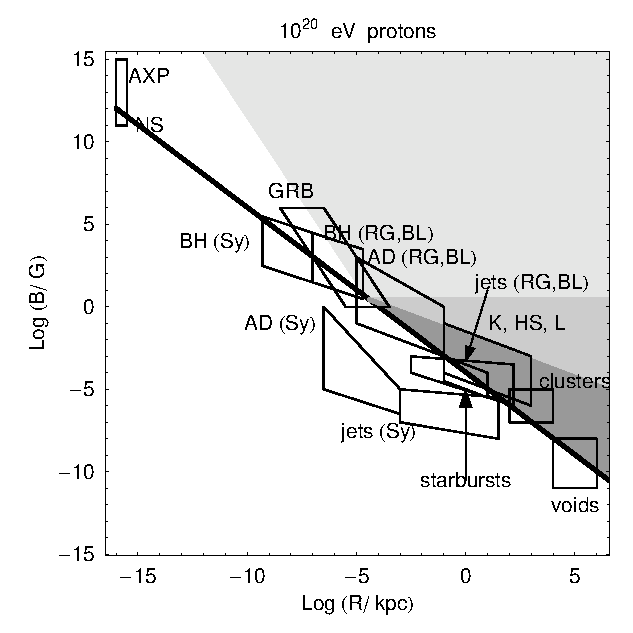
\includegraphics[width=0.5\linewidth]{figures/HillasCriterionProton20}
	\internallinenumbers
	\caption{\textbf{\textit{Hillas criterion for $\SI{1e20}\eV$ protons.}}
		This figure is reproduced here from~\cite{Ptitsyna:2008zs}.
		The black line denotes the region above which objects meet the Hillas criterion.
		The shaded regions show regions allowed for different acceleration scenarios: light gray for one-shot acceleration, gray for one-shot acceleration with synchrotron losses, and dark gray for one-shot acceleration and diffusive shock acceleration.
		Boxes denote the parameters of various astrophysical objects: the central
		parsecs (AD) of active galaxies (low-power Seyfert galaxies (Sy) and powerful radio galaxies (RG) and blazars (BL)), relativistic jets, knots (K), hot spots (HS) and lobes (L) of powerful active galaxies (RG and BL); non-relativistic jets of low-power galaxies (Sy); starburst	galaxies; gamma-ray bursts (GRB); galaxy clusters and inter-cluster voids; immediate
		the neighborhood of neutron stars (NS), anomalous X-ray pulsars and magnetars (AXP).
	}\label{fig:hillasp20}
\end{figure}

Cosmic rays can be observed interacting in the Earth's atmosphere, as they produce extensive particle air-showers whose constituents and products can be observed with a wide range of techniques.
The charged particle products of these interactions have been observed as early as 1912~\cite{hess1912uber}.
These air showers are of particular concern to neutrino detectors as they produce high-energy muons and neutrinos in relative abundance, both of which can be observed by neutrino detectors even with significant shielding and overburden.

When cosmic rays interact with the atmosphere, some nuclear fragments can be produced, but hadronization occurs due to the high energy of the incident cosmic ray and initiates a hadronic particle shower.
As part of the hadronic shower, pions and kaons are produced in abundance.
These subsequently decay or interact in the low-density atmosphere.
Leptonic and semi-leptonic decays of charged pions and kaons that produce muons or neutrinos have a large decay branching fraction, resulting in an abundance of muons and neutrinos in any air shower that begins hadronically.
Decays of charged pions
%($\pi^+\rightarrow\mu^+\nu_\mu$, $\pi^+\rightarrow\mu^+\bar{\nu}_e$, $\pi^+\rightarrow\mu^+\nu_e$, $\pi^+\rightarrow\mu^+\nu_\mu \gamma$, $\pi^+\rightarrow e^+\nu_e$),
($\pi^+\rightarrow\mu^+\nu_\mu$), 
%$K_L^0$ ($K_L^0 \rightarrow \pi^\pm e^\mp \nu_e$, $K_L^0 \rightarrow \pi^\pm \mu^\mp \nu_\mu$), and 
$K_L^0$ ($K_L^0 \rightarrow \pi^\pm e^\mp \nu_e$, $K_L^0 \rightarrow \pi^\pm \mu^\mp \nu_\mu$), and 
%$K^+$ ($K^+\rightarrow \mu^+ \nu_\mu$, $K^+\rightarrow \pi^0 e^+ \nu_e$, $K^+\rightarrow \pi^0 \mu^+ \nu_\mu$, $K^+\rightarrow \mu^+ \nu_\mu \gamma$) 
$K^+$ ($K^+\rightarrow \mu^+ \nu_\mu$, $K^+\rightarrow \pi^0 e^+ \nu_e$, $K^+\rightarrow \pi^0 \mu^+ \nu_\mu$) 
all have direct contributions to the muon and neutrino fluxes; secondary contributions from pion production in kaon decay are also present, particularly for $K_S^0$.
The yield of muons and neutrinos is highly zenith dependent.
This dependence is a result of the interplay between the probability of meson interaction and meson decay.
Unlike those that decay, pions and kaons that interact with the atmosphere or Earth will not produce neutrinos, and decay is much more likely in the low-density atmosphere.
Between the zenith and horizon, the average path length of mesons through the atmosphere increases with zenith angle, thereby increasing the yield of neutrinos for the same flux of cosmic rays.
For this reason, neutrino production from pions and kaons is peaked at the horizon, as shown in \reffig{fig:atmo_zenith}.

\begin{figure}
	\centering
	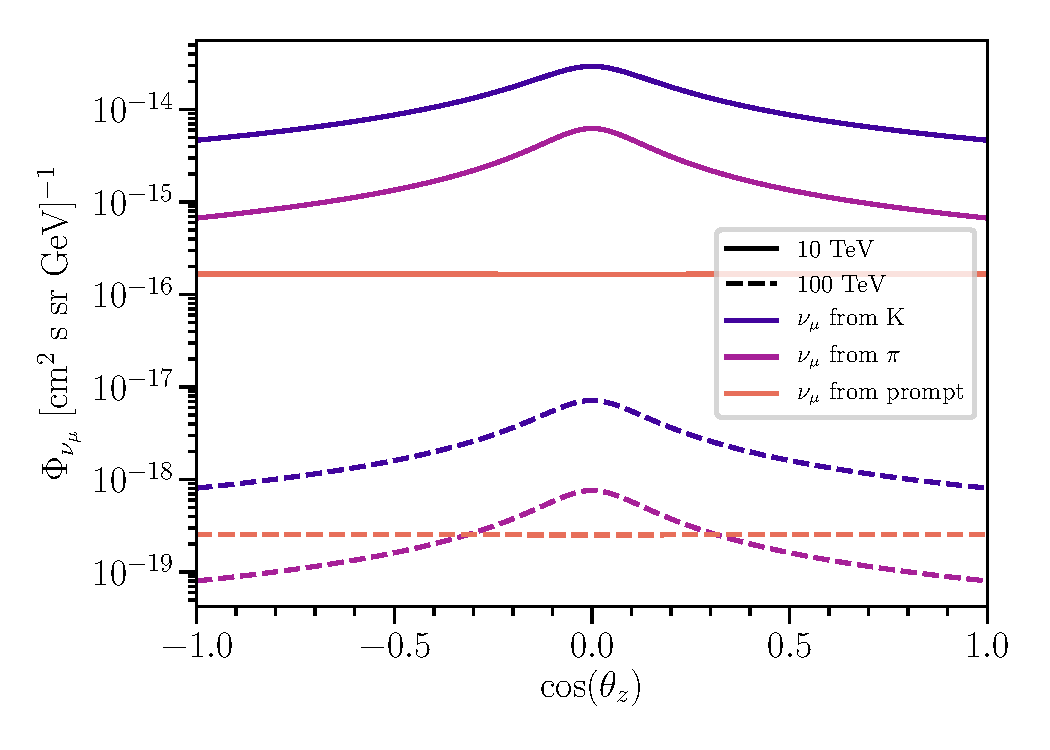
\includegraphics[width=0.7\linewidth]{figures/atm_flux}
	\internallinenumbers
	\caption{\textbf{\textit{Production of atmospheric muon neutrinos.}}
		The atmospheric muon neutrino flux at the Earth's surface is plotted as a function of the zenith angle measured with respect to the IceCube detector center.
		At these high energies above several $\si\TeV$, the production of muon neutrinos is dominated by kaon decays.
		The kaon and pion production is peaked at the horizon, where the path of these particles includes the longest stretch of atmosphere before reaching the Earth.
		This larger path length results in a higher decay probability for these mesons.
		Production from the prompt decay of charmed hadrons has no angular dependence as the decay length of these hadrons is short with respect to the atmosphere for all directions.
	}\label{fig:atmo_zenith}
\end{figure}

Neutrinos can also be produced by charmed hadrons present in air showers.
These hadrons are much shorter-lived than the pion and kaon, and almost invariably decay before interaction.
As the interaction probability for these charmed hadrons is so low, the production of neutrinos from them has practically no dependence on the zenith angle.
This flux of neutrinos is still unobserved, although its spectrum has been predicted ($\sim E^{-2.7}$) and constraints placed on its normalization.
As this atmospheric flux is effectively isotropic, some have suggested that it may be confused for the astrophysical flux.
However, the astrophysical flux can be distinguished by its energy spectrum and the effect described in \refsec{sec:passingfractions}.

Muons produced in these air showers reach the ground where they can be detected, and often penetrate many kilometers into the Earth's surface.
Underground neutrino detectors can, therefore, be sensitive to muon backgrounds despite large overburdens of rock, water, or ice.
On the other hand, Neutrinos have a small interaction cross such that the effective area for neutrinos is approximately $10^6$ times smaller than that for similar energy muons in the few $\si\TeV$ energy regime.
With this small interaction cross section, neutrinos are likely to pass through the Earth without interacting.
Neutrino detectors are then able to observe the atmospheric neutrino flux coming from all directions.
Chapter~\ref{chapter:backgrounds} explores in detail how these backgrounds are estimated for IceCube.

\begin{figure}
	\centering
	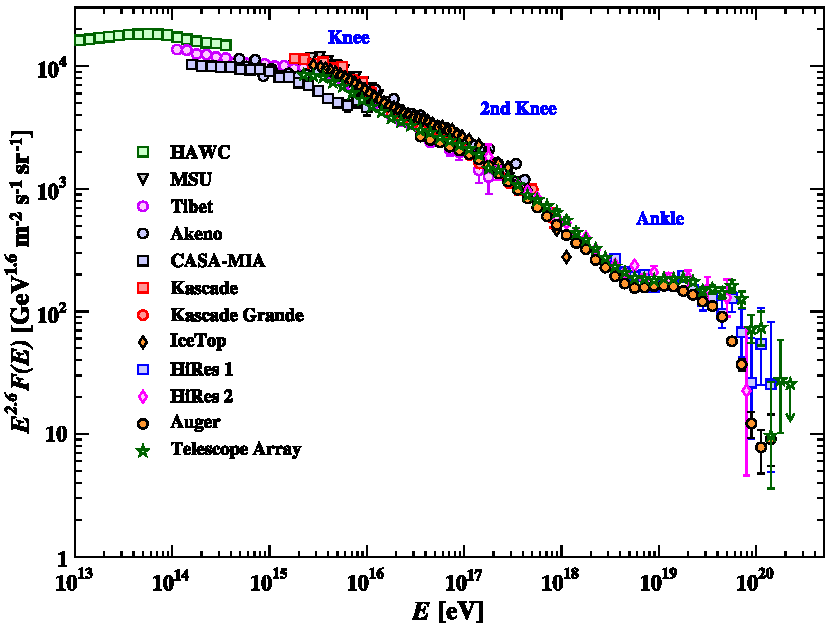
\includegraphics[width=0.8\linewidth]{figures/cosmic_ray_spectrum}
	\internallinenumbers
	\caption{\textbf{\textit{Cosmic Ray Spectrum.}}
		This figure is reproduced here from~\cite{PhysRevD.98.030001}.
		The measured flux of cosmic rays is plotted from a variety of cosmic ray observatories.
		The flux is multiplied by $E^{-2.6}$ to highlight the different spectral features.
		Above $\SI{4e18}\eV$ the harder spectrum of extra-galactic cosmic rays is apparent before the spectrum cuts off.
	}\label{fig:cosmic_ray_spectrum}
\end{figure}

\section{Neutrino interactions and detection}

Neutrinos are the only neutral leptons in the standard model of particle physics.
Although fundamentally, neutrinos only interact through gravity and the exchange of weak bosons, there exists a wide range of processes that dominate the relevant physical behavior of neutrinos at different energy scales.
Such interactions include nuclear capture, inverse beta-decay, quasi-elastic scattering, resonant particle production, coherent elastic scattering, deep inelastic scattering (DIS), and ultra-high energy interactions~\cite{Vannucci:2017rqs,Akimov:2017ade}.
Above $\si\TeV$ neutrino energies, only two known processes remain relevant for detection: DIS and resonant $W$ production.
Deep inelastic scattering refers to processes that probe the fundamental components of hadrons.
For neutrinos, this means the exchange of a weak boson with a quark.
The momentum imparted to the quark will produce a hadronic cascade of secondary particles.
The details of the lepton side of the interaction depend heavily on the species of incident neutrino and weak boson exchanged.
We can divide these DIS interactions into two categories based on the weak boson exchanged.
Interactions involving the exchange of a $Z^0$ are referred to as ``neutral current'' (NC), and those exchanging a $W^+$ or $W^-$ are referred to as ``charged current'' (CC).
Modern techniques for observing neutrino interactions rely on detecting the charged particle products of the initial interaction.
As a consequence of this, the observable energy can be very different for NC and CC events.
Both interactions produce a hadronic cascade, but on the leptonic side of the interaction, NC events have an outgoing neutrino (not observable), while CC events have an outgoing charged lepton (observable).
These two interactions are shown in \reffig{fig:DIS}.

\begin{figure}
	\centering
	\begin{tikzpicture}
	\begin{feynman}
	\vertex (a);
	\vertex [below=of a] (b);
	\vertex [above left=of a] (c) {\(\nu_{l} / \overline \nu_{l}\)};
	\vertex [above right=of a] (d) {\(\nu_{l} / \overline \nu_{l}\)};
	\vertex [below left=of b] (e) {\(u/d\)};
	\vertex [below right=of b] (f) {\(u/d\)};
	\diagram* {
		(c) -- [fermion] (a),
		(a) -- [fermion] (d),
		(e) -- [fermion] (b),
		(b) -- [fermion] (f),
		(a) -- [boson, edge label=\(Z^0\)] (b),
	};
	\end{feynman}
	\end{tikzpicture}
	\begin{tikzpicture}
	\begin{feynman}
	\vertex (a);
	\vertex [below=of a] (b);
	\vertex [above left=of a] (c) {\(\nu_{l} / \overline \nu_{l}\)};
	\vertex [above right=of a] (d) {\(l^\pm\)};
	\vertex [below left=of b] (e) {\(u/d\)};
	\vertex [below right=of b] (f) {\(d/u\)};
	\diagram* {
		(c) -- [fermion] (a),
		(a) -- [fermion] (d),
		(e) -- [fermion] (b),
		(b) -- [fermion] (f),
		(a) -- [boson, edge label=\(W^\pm\)] (b),
	};
	\end{feynman}
	\end{tikzpicture}
	\caption{The neutrino deep inelastic scattering processes NC (left) and CC (right) in matter is shown in the figure above for interactions with nucleon component quarks.
	In both cases, significant momentum can be imparted to the outgoing quark, which will result in the production of a hadronic particle cascade.
	In NC interactions, only the hadronic cascade may be detectable as the interaction product is a neutrino, which is unlikely to undergo another interaction within the detection medium.
	Interactions of the CC variety, on the other hand, produce a charged lepton in addition to the hadronic cascade.
	This charged lepton can also be detected if it receives enough energy.}
	\label{fig:DIS}
\end{figure}

The third interaction relevant above $\si\TeV$ neutrino energies is the resonant production of a $W$ boson, otherwise known as the Glashow resonance (GR)~\cite{Glashow:1960zz}.
In matter on Earth, this process occurs when an anti-electron neutrino combines with an atomic electron to produce an on-shell $W^+$ as shown in~\reffig{fig:glashow}.
If we consider the rest frame of the electron, then this resonance occurs at a neutrino energy of $\SI{6.3}\PeV$.
For atomic electrons we should consider the rest frame of the atom, and in this case there is a Doppler broadening of the resonance of $\sim\SI{20}\percent$ due to the orbital motion of the electrons~\cite{Loewy:2014zva}.
In practice, this broadening is small compared to the energy resolution of modern neutrino detectors that have access to this energy scale, and any further broadening from thermal motion will be even smaller.
The production of a $W^+$ and its subsequent decay can result in either a hadronic shower similar to a NC interaction, or a leptonic final state similar to a CC interaction.
These two possibilities correspond to the hadronic and leptonic decay modes of the $W$, respectively.

The cross section of these processes is shown as a function of the neutrino energy in \reffig{fig:nuxs}.
The growth of the cross section with energy counteracts the falling neutrino spectrum to only a small degree.
Despite the large cross section, only a few Glashow resonance events are expected in $\SI{10}\year$ of IceCube detector operation due to the comparably low neutrino flux at these energies.
Absorption of neutrinos in the Earth becomes significant above $\sim\SI{1}\TeV$, and is notably peaked near the $\SI{6.3}\PeV$ resonance energy.

\begin{figure}
	\centering
	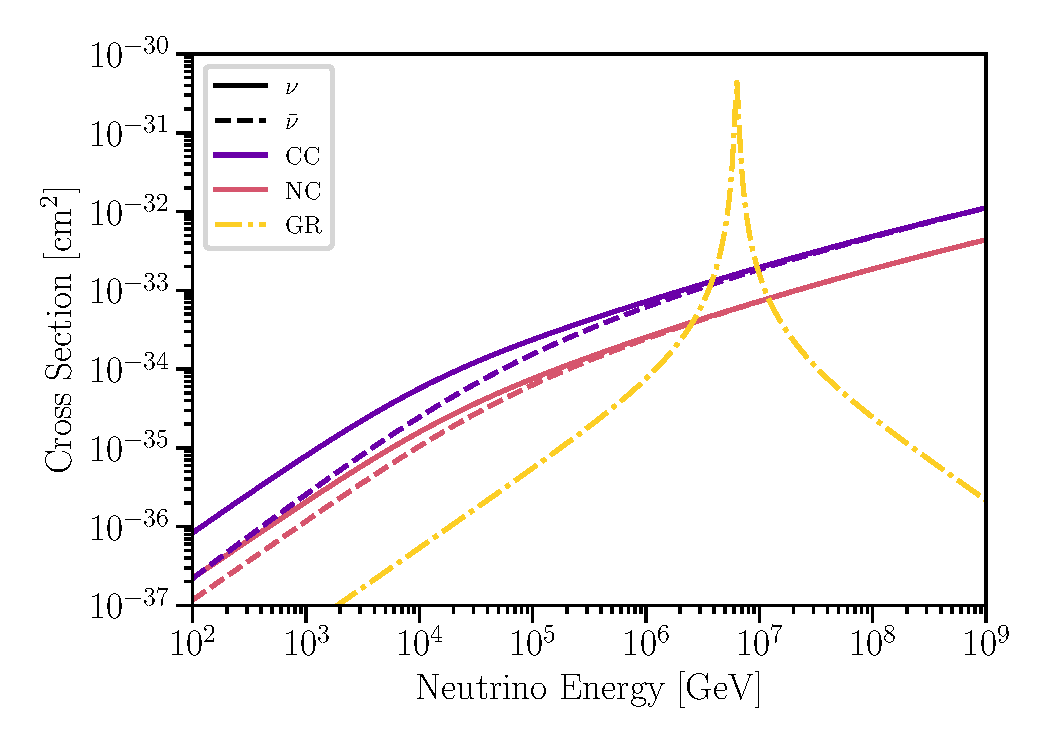
\includegraphics[width=0.8\linewidth]{figures/xs}
	\internallinenumbers
	\caption{\textbf{\textit{Neutrino interaction cross sections.}}
	Charged current (CC), neutral current (NC), and Glashow resonance (GR) cross sections are shown as a function of neutrino energy.
	The CC and NC cross sections come from~\cite{CooperSarkar:2011pa}, while the GR cross sections are computed using the forms in~\cite{Gandhi:1995tf} and corrected for the Doppler shift of electrons in the molecular orbitals of water~\cite{Loewy:2014zva}.
	}\label{fig:nuxs}
\end{figure}

\begin{figure}
	\centering
	\begin{tikzpicture}
	\begin{feynman}
	\vertex (a);
	\vertex [right=of a] (b);
	\vertex [above left=of a] (c) {\(\overline \nu_{e}\)};
	\vertex [below left=of a] (d) {\(e^-\)};
	\diagram* {
		(c) -- [fermion] (a),
		(a) -- [fermion] (d),
		(a) -- [boson, edge label=\(W^+\)] (b),
	};
	\end{feynman}
	\end{tikzpicture}
	\caption{The production of an on-shell $W^+$ boson through the combination of an anti-electron neutrino and electron.
		This resonant process occurs at neutrino energies around $\SI{6.3}\PeV$.}
	\label{fig:glashow}
\end{figure}

Through either a NC interaction or the hadronic decay of a $W$ boson, neutrinos can induce a hadronic shower.
In a hadronic shower, both charged hadrons and leptons are produced, which can be detected through well-established methods.
Charged current interactions produce a hadronic shower by imparting momentum to a quark that is then hadronized, although the charged lepton produced in the interaction is also detectable and can significantly alter the event's detection signature.

Through either a CC interaction or the leptonic decay of a $W$ boson, neutrinos can produce a detectable charged lepton, although the detection signature differs depending on the charged lepton's flavor.
Focusing on dense detection media like ice or water, the three flavors of charged leptons' detection signatures are as follows.
High energy electrons and positrons immediately interact with the detection media to initiate an electromagnetic cascade where charged leptons and high energy photons are alternately produced by one another.
This electromagnetic cascade develops over $\sim10$ radiation lengths (about $\sim\SI{5}\m$ in total) at $\SI{10}\TeV$ with a lateral extension of $\sim\SI{20}\cm$ (twice the Molière radius), expanding within the dense detection medium, and has an extreme directional bias because of the momentum of the first charged lepton.

Muons from high energy neutrino interactions do not interact as readily as electrons and positrons due to their larger mass.
Instead, muons can travel several kilometers in dense media before losing enough energy to quickly decay.
Along their entire path length, muons lose energy by interacting with the detection medium.
These ``energy loss'' interactions include ionization, electron-positron pair production, bremsstrahlung, and photo-nuclear interactions.
Although these processes are highly stochastic, the average energy loss of muons approximately follows $-dE/dx=a+bE$ where $a$ is determined by the ionization energy losses and $b$ is defined by the other processes.
In general, $a$ and $b$ are both functions of muon energy $E$, but this linear approximation where $a$ and $b$ are constant holds locally as both are slowly varying as a function of $E$.
For muon energies above $\SI{1}\TeV$, the so-called ``radiative'' term $bE$ dominates the average energy losses.
Figure~\ref{fig:energy_losses} shows the energy loss rate for the different processes.
Once the radiative losses have taken over above $\sim\SI{1}\TeV$, the losses grow exponentially with energy.

\begin{figure}
	\centering
	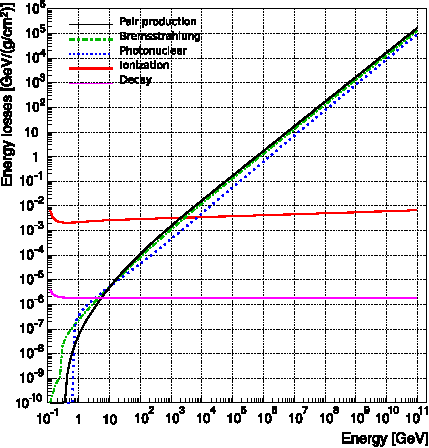
\includegraphics[width=0.8\linewidth]{figures/energy_losses}
	\internallinenumbers
	\caption{\textbf{\textit{Muon Energy Losses}}
		The muon energy loss rate computed for water is plotted as a function of the muon energy for the five different loss processes.
		This figure is reproduced here from~\cite{Koehne:2013gpa}.
		Radiative energy losses dominate above $\sim\SI{1}\TeV$.
		Although it is a smaller contribution to the energy losses, photo-nuclear interactions are the main source of uncertainty above $\sim\SI{1}\TeV$.
	}\label{fig:energy_losses}
\end{figure}

The strong dependence of the energy loss rate on muon energy means that the energy lost while traversing the detector can be used to estimate a muon's energy.
For simple observables like the total energy lost over $\SI{1}\km$ the stochastic energy losses introduce large variations between muons of the same energy, reducing their power as a proxy for the muon energy.
Figure~\ref{fig:muon_energy} shows the energy of muons lost within $\SI{1}\km$ of ice; a distribution with very long tails.
In practice the muon energy can currently be determined to within a factor of $2$, however improved techniques that take advantage of more detailed information may achieve a resolution as small as $\SI{10}\percent$ in the future.

\begin{figure}
	\centering
	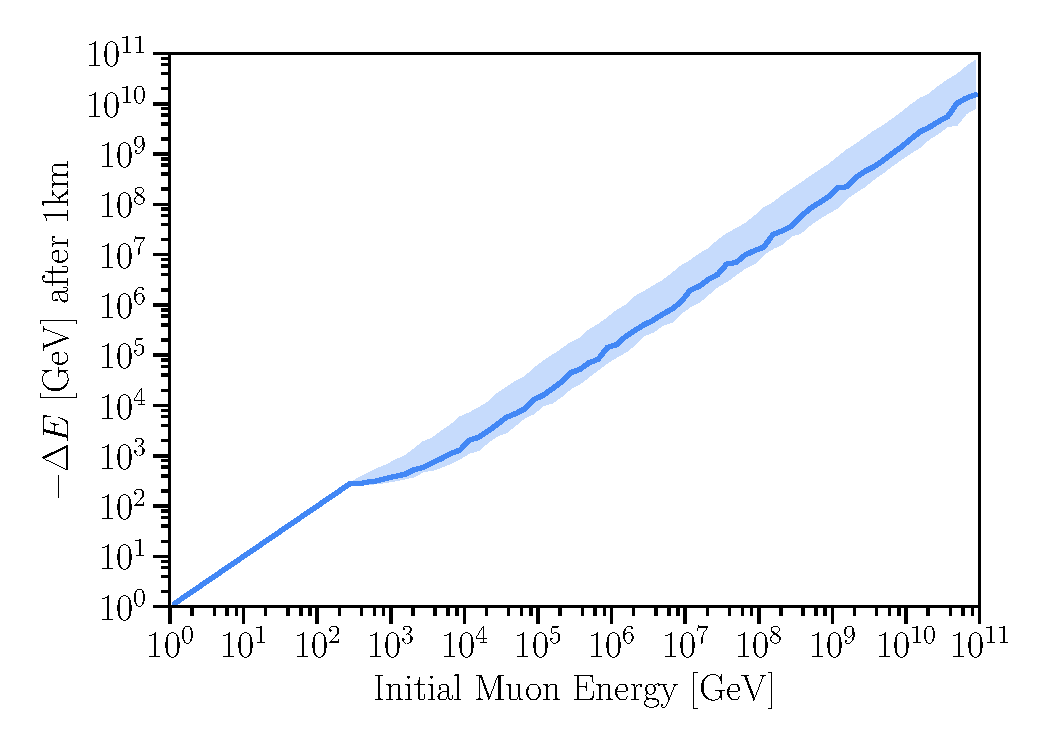
\includegraphics[width=0.8\linewidth]{figures/muon_energy}
	\internallinenumbers
	\caption{\textbf{\textit{Muon energy loss in $\SI{1}\km$ of ice.}}
		Muons are propagated through $\SI{1}\km$ of ice, and their lost energy recorded.
		For each initial muon energy, the MAP and $\SI{90}\percent$ HPD region are plotted here.
		There is a strong correlation between the initial energy and energy lost.
		However, the distribution has very long tails, making a precise determination of the muon energy based on this observable impossible.
		Below a few hundred $\si\GeV$ muons lose all of their energy within $\SI{1}\km$ of ice, narrowing the distribution of $\Delta E$.
	}\label{fig:muon_energy}
\end{figure}

Taus produced through a CC interaction, or the leptonic decay of a $W$ boson are also detectable.
The short decay length of a tau, $\SI{50}\meter / \si\PeV$, means it is likely to decay very close to the neutrino interaction vertex.
Taus decay hadronically to produce a hadronic shower with a branching ratio of $\SI{64.79}\percent$.
The tau's leptonic decay modes are decay to a charged lepton and corresponding neutrino of either electron or muon flavor.
In the electron case, an electromagnetic shower results; whereas a far traveling muon is produced in the muon case.
For taus produced via the decay of a $W$ boson, the event is indistinguishable from taus produces via CC and NC interactions other than by the resonance energy at which this process occurs.
Although a tau may traverse tens of meters, which is detectable by IceCube, the energy losses are still negligible over these distances.

From the wide variety of methods for detecting charged particles, water Cherenkov detectors are most common for detecting neutrinos in this high-energy regime above $\SI{1}\TeV$.
Water Cherenkov detectors have the advantage that their detection medium is both abundant and inexpensive, a major motivator in the design of IceCube.
Cherenkov radiation results from charged particles propagating through a dielectric medium faster than the phase velocity of light.
As charged particles pass through the dielectric material, the ionization of the medium induces the emission of light.
For particles faster than the phase velocity of emitted light, the emission forms a conical coherent wave front at a well-defined angle to the particle's path.

\begin{figure}
	\centering
	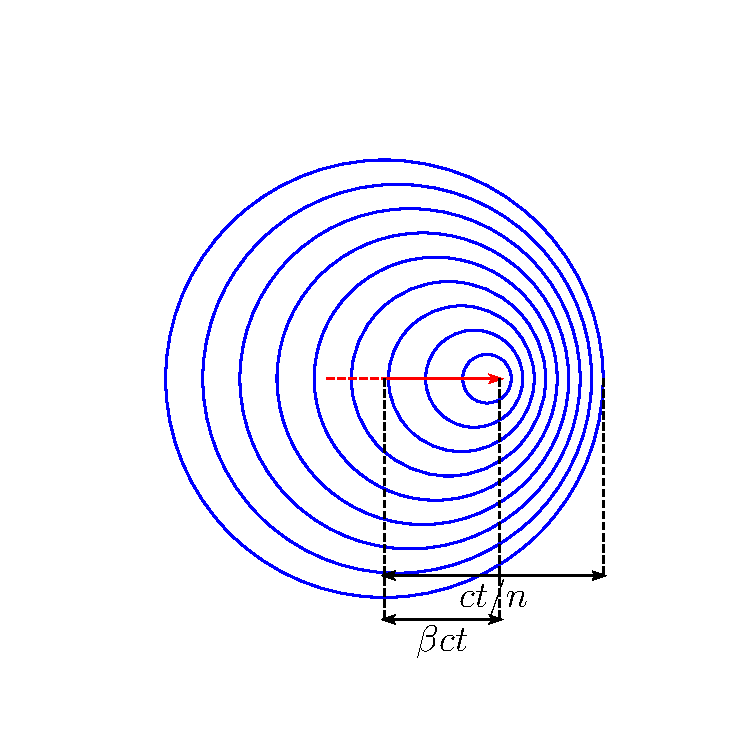
\includegraphics[width=0.45\linewidth]{figures/no_cherenkov}
	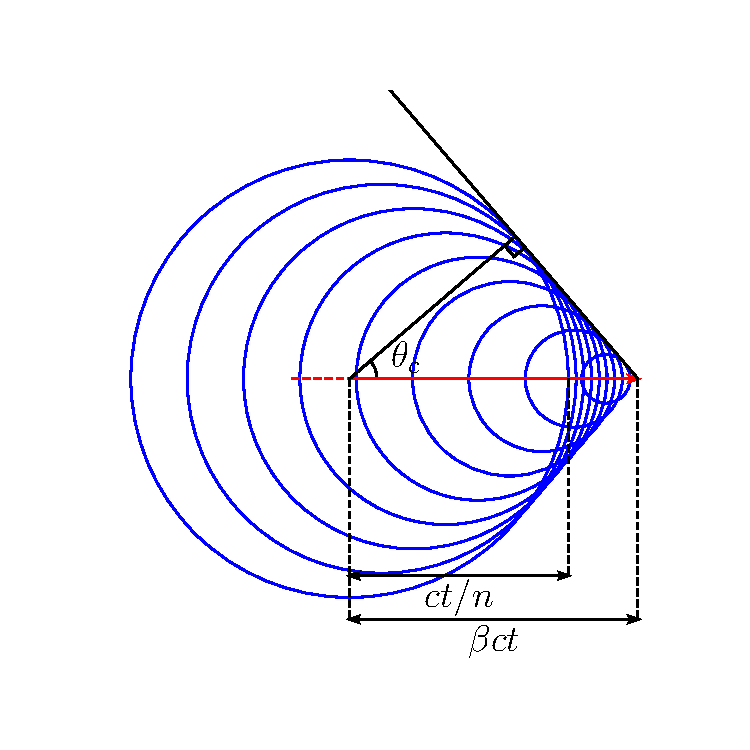
\includegraphics[width=0.45\linewidth]{figures/cherenkov}
	\internallinenumbers
	\caption{\textbf{\textit{Cherenkov radiation.}}
		This diagram shows the photon wavefronts as a charged particle moves through a dielectric medium.
		On the left for $\beta < 1/n$ and on the right for $\beta \geq 1/n$.
		The Cherenkov angle $\theta_c$ is shown on the right and describes a ray perpendicular to the coherent wavefront.
		In the Antarctic ice the Cherenkov angle $\theta_c=\SI{40.72}\degree$.
	}\label{fig:cherenkov}
\end{figure}

These detectors use Cherenkov radiation to detect particles, but the high-energy secondary charged leptons themselves contribute only a small fraction of the Cherenkov photons.
The tertiary particle showers produce most of the Cherenkov photons that these leptons give rise to when they lose energy in the detection medium.
This increased light-yield allows detectors to be sparsely instrumented while maintaining detection efficiency and reconstruction quality.

Water Cherenkov detectors often make use of photo-multiplier-tubes (PMTs) to detect Cherenkov photons.
PMTs have a thin photo-cathode held at a high-voltage differential with respect to an anode; this allows the production and acceleration of a photo-electron when photons pass through the photo-cathode.
Accelerated photo-electrons hurtle towards an amplification stage composed of many dynodes, each held at a large voltage difference to the adjacent dynodes.
This setup allows a single photo-electron to produce many secondary electrons upon interaction with a dynode, starting an exponential cascade of electrons across the dynode stages.
The resulting cascade of electrons is amplified with respect to the original signal enough to be detected electronically as a voltage change.
In this way, PMTs can be sensitive to single photons, provided one can reach the photo-cathode and produce a photo-electron.
\chapter{The IceCube Neutrino Observatory}

\section{Neutrino interactions and detection}

\section{The IceCube detector}

\begingroup
\graphicspath{{results/HESE_Final_Paper/}}
\subfile{results/HESE_Final_Paper/sections/detectorselection/detector}
\endgroup

\chapter{Searching for astrophysical neutrinos}

\section{Event selection\label{sec:selection}}
\begingroup
\graphicspath{{results/HESE_Final_Paper/}}
\chapter{Searching for astrophysical neutrinos}

\section{Event selection\label{sec:selection}}
\begingroup
\graphicspath{{results/HESE_Final_Paper/}}
\chapter{Searching for astrophysical neutrinos}

\section{Event selection\label{sec:selection}}
\begingroup
\graphicspath{{results/HESE_Final_Paper/}}
\input{results/HESE_Final_Paper/sections/detectorselection/selection}
\endgroup

\section{Reconstruction and simulation}
\begingroup
\graphicspath{{results/HESE_Final_Paper/}}
\input{results/HESE_Final_Paper/sections/reconstruction}
\endgroup

\section{Systematic uncertainties and statistical treatment\label{sec:uncertainties}}
\subsection{Detector systematic uncertainties\label{sec:detector_systematics}}
\begingroup
\graphicspath{{results/HESE_Final_Paper/}}
\input{results/HESE_Final_Paper/sections/uncertainties/systematics}
\endgroup

\subsection{Statistical treatment\label{sec:statistics}}
\begingroup
\graphicspath{{results/HESE_Final_Paper/}}
\input{results/HESE_Final_Paper/sections/uncertainties/statistics}
\endgroup

\endgroup

\section{Reconstruction and simulation}
\begingroup
\graphicspath{{results/HESE_Final_Paper/}}
\chapter{Event reconstruction and simulation}\label{chapter:reconstruction}
\begingroup
\graphicspath{{results/HESE_Final_Paper/}}
\input{results/HESE_Final_Paper/sections/reconstruction}
\endgroup
\endgroup

\section{Systematic uncertainties and statistical treatment\label{sec:uncertainties}}
\subsection{Detector systematic uncertainties\label{sec:detector_systematics}}
\begingroup
\graphicspath{{results/HESE_Final_Paper/}}
\input{results/HESE_Final_Paper/sections/uncertainties/systematics}
\endgroup

\subsection{Statistical treatment\label{sec:statistics}}
\begingroup
\graphicspath{{results/HESE_Final_Paper/}}
\chapter{Statistics}\label{chapter:statistics}

\section{Systematic uncertainties and statistical treatment\label{sec:uncertainties}}
\subsection{Detector systematic uncertainties\label{sec:detector_systematics}}
\begingroup
\graphicspath{{results/HESE_Final_Paper/}}
\input{results/HESE_Final_Paper/sections/uncertainties/systematics}
\endgroup

\subsection{Statistical treatment\label{sec:statistics}}
\begingroup
\graphicspath{{results/HESE_Final_Paper/}}
\input{results/HESE_Final_Paper/sections/uncertainties/statistics}
\endgroup

\section{Dealing with limited simulation samples\label{sec:limited_simulation}}
The contents of this section is reproduced here with minor modifications from a collaborative work with Carlos A. Argüelles, and Tianlu Yuan~\cite{Arguelles:2019izp}.

\begingroup
\graphicspath{{results/mcllh_paper/}}
\input{results/mcllh_paper/sections/introduction}
\endgroup

\subsection{The Poisson likelihood and previous work\label{sec:mc_intro}}
\begingroup
\graphicspath{{results/mcllh_paper/}}
\input{results/mcllh_paper/sections/previous_work/poisson}
\endgroup

\subsubsection{The Barlow-Beeston likelihood}
\begingroup
\graphicspath{{results/mcllh_paper/}}
\input{results/mcllh_paper/sections/previous_work/bb}
\endgroup

\subsubsection{Uncertainties in the large-sample limit}
\begingroup
\graphicspath{{results/mcllh_paper/}}
\input{results/mcllh_paper/sections/previous_work/chi2}
\endgroup

\subsection{Generalization of the Poisson likelihood\label{sec:generalization_poisson}}
\begingroup
\graphicspath{{results/mcllh_paper/}}
\input{results/mcllh_paper/sections/generalized_poisson/generalized_poisson}
\endgroup

\subsubsection{Derivation of $\like (\lambda|\vecw(\vectheta))$ for identical weights\label{sec:constructing}}
\begingroup
\graphicspath{{results/mcllh_paper/}}
\input{results/mcllh_paper/sections/generalized_poisson/identical_weights}
\endgroup

\subsubsection{Extension to arbitrary weights\label{sec:extending}}
\begingroup
\graphicspath{{results/mcllh_paper/}}
\input{results/mcllh_paper/sections/generalized_poisson/arbitrary_weights}
\endgroup

\subsubsection{The effective likelihood\label{sec:effective}}
\begingroup
\graphicspath{{results/mcllh_paper/}}
\input{results/mcllh_paper/sections/generalized_poisson/effective_likelihood}
\endgroup

\subsubsection{A family of likelihoods\label{sec:priors}}
\begingroup
\graphicspath{{results/mcllh_paper/}}
\input{results/mcllh_paper/sections/generalized_poisson/family}
\endgroup

\subsubsection{Convergence of the effective likelihood\label{sec:llhconvergence}}
\begingroup
\graphicspath{{results/mcllh_paper/}}
\input{results/mcllh_paper/sections/generalized_poisson/convergence}
\endgroup

\subsubsection{Behavior of the effective likelihood\label{sec:llhbehavior}}
\begingroup
\graphicspath{{results/mcllh_paper/}}
\input{results/mcllh_paper/sections/generalized_poisson/behavior}
\endgroup

\subsection{Example and performance\label{sec:example}}
\begingroup
\graphicspath{{results/mcllh_paper/}}
\input{results/mcllh_paper/sections/example/example}
\endgroup

\subsubsection{Point estimation\label{sec:pointestimation}}
\begingroup
\graphicspath{{results/mcllh_paper/}}
\input{results/mcllh_paper/sections/example/point_estimation}
\endgroup

\subsubsection{Coverage\label{sec:coverage}}
\begingroup
\graphicspath{{results/mcllh_paper/}}
\input{results/mcllh_paper/sections/example/coverage}
\endgroup

\subsubsection{Posterior distributions\label{sec:posterior}}
\begingroup
\graphicspath{{results/mcllh_paper/}}
\input{results/mcllh_paper/sections/example/posterior}
\endgroup

\subsubsection{Performance\label{sec:performance}}
\begingroup
\graphicspath{{results/mcllh_paper/}}
\input{results/mcllh_paper/sections/example/performance}
\endgroup

\subsection{Conclusion\label{sec:llhconclusion}}
\begingroup
\graphicspath{{results/mcllh_paper/}}
\input{results/mcllh_paper/sections/conclusion}
\endgroup

\subsection{Summary of likelihood formulas\label{sec:llhtable}}
\begingroup
\graphicspath{{results/mcllh_paper/}}
\input{results/mcllh_paper/appendices/formulas}
\endgroup
\FloatBarrier
\section{Frequentist confidence intervals with nuisance parameters and limited simulation}\label{sec:low_stats_confidence_intervals}

Frequentist and Bayesian techniques deal with different two different kinds of probability.
In frequentist statistics, the relevant probability is the frequency of the outcome of a repeatable experiment.
Under this framework the important concepts are parameter estimation, confidence intervals, and statistical tests.
In Bayesian statistics, the relevant probabilities come from the application of Bayes theorem which means we can define the probability density of parameters.
This definition of the parameter p.d.f. is applicable to the same problems parameter estimation, interval construction, and statistical tests but comes at the cost of defining ``prior belief'' about parameters.

In this section we will ignore the problem of statistical tests, instead focusing on the common features that underpin parameter estimation and interval construction.
Generally in parameter estimation and interval construction there are two sets of parameters, parameters of interest $\vec\theta$ and nuisance parameters $\vec\eta$.
Fundamentally there is no distinction between these two kinds of parameters.
The difference is only in which parameters we want to infer information about.

For both parameter estimation and interval construction the likelihood function is central.
The likelihood function reflects the plausibility of model parameters given observed data and is defined as $\like(\vec\theta, \vec\eta|\textrm{data}) = p(\textrm{data}|\vec\theta, \vec\eta)$.
Where $p(\textrm{data}|\vec\theta, \vec\eta)$ is the probability of the data given the model parameters.
A useful technique to eliminate nuisance parameters is the profile likelihood technique.
Dropping the explicit notational dependence on data, the profile likelihood function is defined as
\begin{linenomath*}
	\begin{equation}
	\tilde{\like}^\texttt{profile}(\vec\theta) = \max_{\vec\eta} \like(\vec\theta,\vec\eta),
	\label{eq:likelihood_profile}
	\end{equation}
\end{linenomath*}
where often the negative log of the function is maximized in place of the function for computational reasons.
The profile likelihood is then only a function of the parameters of interest.
Parameter estimation can be performed by maximizing the profile likelihood to obtain the ``best-fit'' parameters
\begin{linenomath*}
	\begin{equation}
	\hat{\vec\theta} = \argmax_{\vec\theta} \tilde{\like}^\texttt{profile}(\vec\theta).
	\label{eq:best_fit}
	\end{equation}
\end{linenomath*}
This best-fit point in the parameter space is a derived property of the likelihood function.
However, the same procedure can be performed with other functions to the same effect.
In general a minimization procedure is used, and we refer to these functions as ``test-statistics'' (TS).
A particularly useful TS is derived directly from the profile likelihood technique,
\begin{linenomath*}
	\begin{equation}
	\TS(\vec\theta) = -2\log{\left(\frac{\tilde{\like}^\texttt{profile}(\vec\theta)}{\tilde{\like}^\texttt{profile}(\hat{\vec\theta})}\right)}.
	\end{equation}
\end{linenomath*}
Using this TS to perform parameter estimation through minimization is mathematically equivalent to maximizing the likelihood, however, this form will prove to be uniquely useful for interval construction.

Since frequentist statistics deals with the frequency of outcomes from repeated experiments we can use the TS that results from repeated experiments to construct probabilities.
Consider for a moment a single point in the parameter space $\vec\theta_0$.
At this point in the parameter space there is a distribution of data that can be observed, and therefore a distribution of TS functions.
Instead of considering the distribution of TS functions originating from this point, we can simplify the picture by looking at the TS function only evaluated at this point $\TS(\vec\theta_0)$.
This gives us a distribution of TS values for this point in the parameter space that may look like~\reffig{fig:TS_dist}.
\begin{figure}
	\centering
	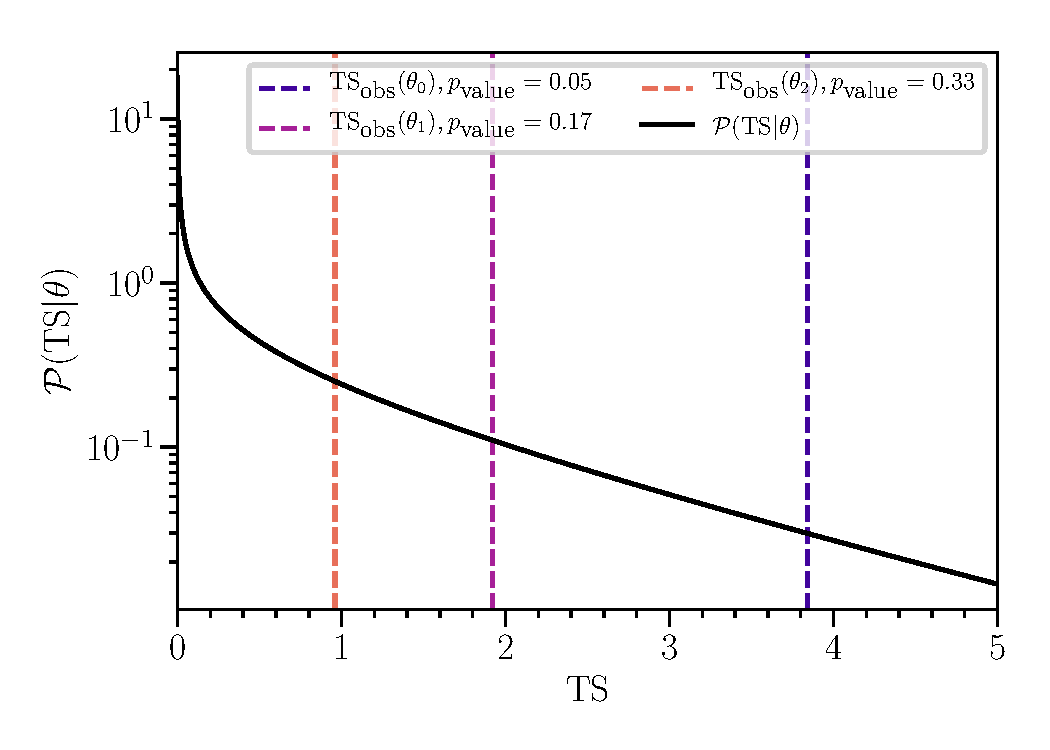
\includegraphics[width=0.8\linewidth]{figures/TS_dist}
	\caption{\textbf{\textit{Test statistic distribution.}} An example of a test statistic distribution.
	Such distributions tend to have the bulk of their mass close to the lower boundary with a long tail.
	Lower values indicate better statistical compatibility with the data.
	}
	\label{fig:TS_dist}
\end{figure}
It is important to note that for the profile likelihood TS and similar statistics a smaller TS value indicates better compatibility with the data.
For this reason many statistical tests are constructed using a single tail significance, by comparing the TS from a single experiment to a background TS distribution and reporting a p-value that is the fraction of the TS distribution greater than the observed TS.

This procedure can be extended to construct intervals by considering the TS distributions of every point in parameter space and comparing to the observed TS function.
Consider the one-dimensional case where there is a TS distribution for each value of the parameter, illustrated in~\reffig{fig:TS_dists_1d}
\begin{figure}
	\centering
	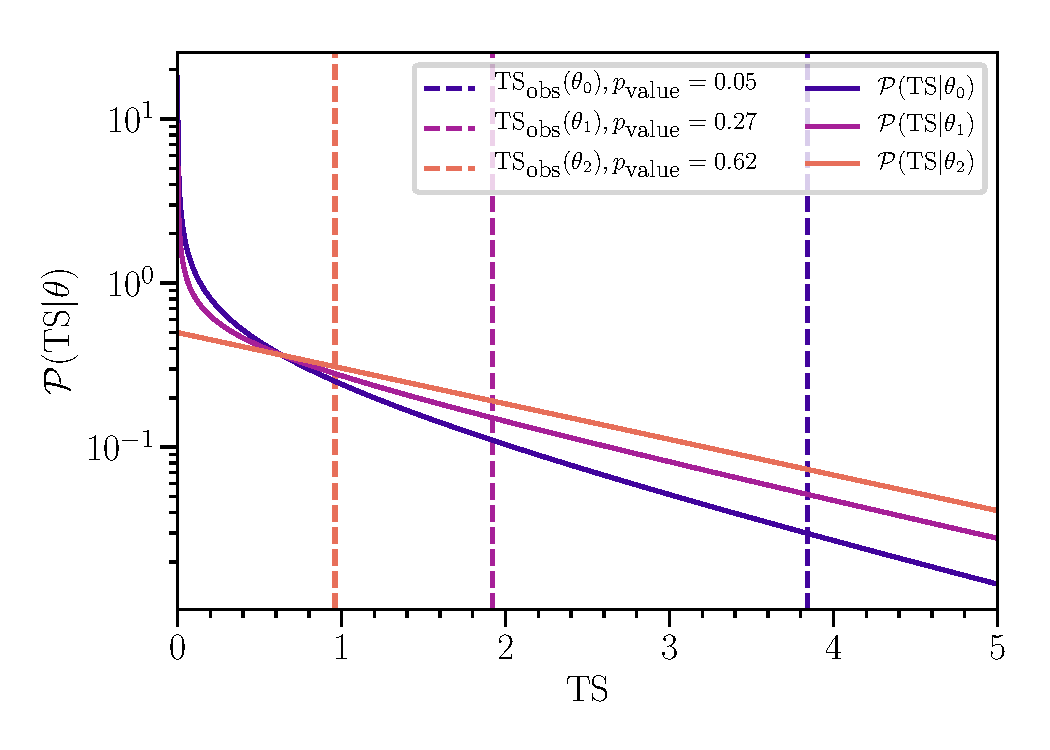
\includegraphics[width=0.8\linewidth]{figures/TS_dists_1d}
	\caption{\textbf{\textit{One-dimensional test-statistic distribution comparison.}} An example of the test statistic distributions as a function of a single parameter.
	}
	\label{fig:TS_dists_1d}
\end{figure}
We can construct an interval that will contain the true value of the parameter a fraction of the time $\alpha$ for repeated experiments.
This interval is the collection of points in the one-dimensional parameter space where the TS at that point is greater than the $\alpha$ quantile of the corresponding TS distribution.
If the TS distribution is the same for all points in parameter space, the interval construction can procedurally be thought of as drawing a horizontal line at the appropriate threshold and only including points that lie below the line.
Varying TS distributions modify this procedure to the comparison of two curves.
This procedure is not limited to one-dimension but can be extended to an arbitrary number of parameters of interest to construct n-dimensional regions with the same properties.

There is however an important caveat to this construction that appears when we consider nuisance parameters.
In order for the intervals to have the desired properties, the observed TS must be greater than the threshold for all possible values of the nuisance parameters.
This ultimatum presents several challenges.
Nuisance parameters can often have a broad or even unbounded range of allowed values, meaning if the effect of nuisance parameters does not taper off at the extrema then almost all intervals are guaranteed to be empty.
From a practical standpoint, computing the TS distributions for many points in parameter space is often done via Monte-Carlo and is computationally expensive.
Adding additional dimensions to the parameter space for which we must compute TS distributions exponentially increases the computation time.

To combat these issues we can limit our interval construction to be valid for values of the nuisance parameters that are ``reasonable''.
There are several methods for doing this, but we can split them into two categories: pure frequentist, and frequentist-Bayesian hybrid.
In the pure frequentist approaches we can either choose a single value of the nuisance parameters, or work with a limited range of the nuisance parameter values.
For the single value approach either nominal values are chosen before looking at the data, or estimators of the nuisance parameters are used to choose their values.
This approach benefits from simplicity, but fails if the test-statistic distributions vary rapidly with changes to the nuisance parameters for values that we might consider ``reasonable''.
A more expensive but robust approach is to explore the behavior of TS distributions for a limited range of the nuisance parameter values, which can be chosen {\it a priori} or from data-based bounds on the nuisance parameters.
If we are willing to consider a hybrid approach, then some more pragmatic options are available.

Although Bayesian methods could be used to choose a single point in parameter space from which to generate the TS distributions, the more interesting application is one that uses a distribution in parameter space.
In Bayesian statistics we can directly assign a probability density to the points in parameter space, either based on our prior information, or directly informed by the posterior distribution, from this extended perspective the probability of certain nuisance parameter values is of interest when considering the frequency of TS values for different parameters of interest.
The prior case is simple in that we sample the from the nuisance parameter priors when generating the TS distribution which allows us to account for variability introduced by the nuisance parameters without relying on hard cutoffs or biasing our inferences with parameter values that are unrealistic.
This prior based technique is well motivated if the priors are derived from external observations, however in the case where nuisance parameters have broad or ``uninformative'' priors this motivation and benefit may break down.
In some cases we expect nuisance parameters to be heavily constrained by the same data sample used to investigate the parameters of interest, so a different approach is merited.
The alternative is to use the posterior distribution to construct our nuisance parameter p.d.f.
Ideally a posterior distribution would be computed for each point in the parameters of interest space by fixing those parameters of interest.
In this way the nuisance parameter posterior used for sampling depends on the point in parameter space we are examining.

With the possible solutions available, we can now look at the problem of limited simulation size when generating test statistic distributions.
As explored in~\refsec{sec:limited_simulation} for binned Poisson likelihood problems, the real expectation in data or simulation for the number of events in a bin is not a known quantity.
Because the real expectations are not known, it is impossible to exactly model the distribution of TS that are expected for a particular point in the parameter space.
However, as~\refsec{sec:limited_simulation} also explored, limited simulation can be modeled with nuisance parameters so the techniques discussed above can be applied directly to the problem.
The ``single point in parameter space'' approach fails to address the additional uncertainty present in this case.
Allowing for unbounded variation of the bin expectations fails as it is guaranteed to produce empty intervals.
Bounding of the bin expectations within a reasonable range provides manageable intervals, but the dimensionality of the problem makes this computationally unfeasible beyond a handful of bins.
Unfortunately this excludes all the ``classic'' frequentist solutions to this problem.
The hybrid Bayesian-frequentist methods in this case provide a tractable solution that accounts for the additional uncertainty.
We can make use of the treatment described in~\refsec{sec:effective}, where the bin expectation is derived to be gamma distributed, and the expected number of data events modeled to be Poisson distributed once this expectation is known.
Practically this can be achieved by sampling data events from $\mcl$, or through a two step process where the expectation is sampled from a gamma distribution $\gprob(\lambda;\agpar, \bgpar)$ where $\agpar = \frac{\mu^2}{\sigma^2}+1~\textmd{and}~\bgpar=\frac{\mu}{\sigma^2}$, and the data events are sampled from a Poisson distribution $\frac{\lambda^{k}e^{-\lambda}}{k!}$.
It is important to note that this procedure only applies to variations in the data and should not be used to vary simulation expectations.
This is because the TS distribution is intended to model variations in the data, whereas the simulation used for analysis is fixed.
Combined with a similar hybrid treatment for other nuisance parameters, this provides a more complete accounting of the uncertainties given the available modeling.
\endgroup

\endgroup

\section{Reconstruction and simulation}
\begingroup
\graphicspath{{results/HESE_Final_Paper/}}
\chapter{Event reconstruction and simulation}\label{chapter:reconstruction}
\begingroup
\graphicspath{{results/HESE_Final_Paper/}}
\chapter{Event reconstruction and simulation}\label{chapter:reconstruction}
\begingroup
\graphicspath{{results/HESE_Final_Paper/}}
\input{results/HESE_Final_Paper/sections/reconstruction}
\endgroup
\endgroup
\endgroup

\section{Systematic uncertainties and statistical treatment\label{sec:uncertainties}}
\subsection{Detector systematic uncertainties\label{sec:detector_systematics}}
\begingroup
\graphicspath{{results/HESE_Final_Paper/}}
\input{results/HESE_Final_Paper/sections/uncertainties/systematics}
\endgroup

\subsection{Statistical treatment\label{sec:statistics}}
\begingroup
\graphicspath{{results/HESE_Final_Paper/}}
\chapter{Statistics}\label{chapter:statistics}

\section{Systematic uncertainties and statistical treatment\label{sec:uncertainties}}
\subsection{Detector systematic uncertainties\label{sec:detector_systematics}}
\begingroup
\graphicspath{{results/HESE_Final_Paper/}}
\input{results/HESE_Final_Paper/sections/uncertainties/systematics}
\endgroup

\subsection{Statistical treatment\label{sec:statistics}}
\begingroup
\graphicspath{{results/HESE_Final_Paper/}}
\chapter{Statistics}\label{chapter:statistics}

\section{Systematic uncertainties and statistical treatment\label{sec:uncertainties}}
\subsection{Detector systematic uncertainties\label{sec:detector_systematics}}
\begingroup
\graphicspath{{results/HESE_Final_Paper/}}
\input{results/HESE_Final_Paper/sections/uncertainties/systematics}
\endgroup

\subsection{Statistical treatment\label{sec:statistics}}
\begingroup
\graphicspath{{results/HESE_Final_Paper/}}
\input{results/HESE_Final_Paper/sections/uncertainties/statistics}
\endgroup

\section{Dealing with limited simulation samples\label{sec:limited_simulation}}
The contents of this section is reproduced here with minor modifications from a collaborative work with Carlos A. Argüelles, and Tianlu Yuan~\cite{Arguelles:2019izp}.

\begingroup
\graphicspath{{results/mcllh_paper/}}
\input{results/mcllh_paper/sections/introduction}
\endgroup

\subsection{The Poisson likelihood and previous work\label{sec:mc_intro}}
\begingroup
\graphicspath{{results/mcllh_paper/}}
\input{results/mcllh_paper/sections/previous_work/poisson}
\endgroup

\subsubsection{The Barlow-Beeston likelihood}
\begingroup
\graphicspath{{results/mcllh_paper/}}
\input{results/mcllh_paper/sections/previous_work/bb}
\endgroup

\subsubsection{Uncertainties in the large-sample limit}
\begingroup
\graphicspath{{results/mcllh_paper/}}
\input{results/mcllh_paper/sections/previous_work/chi2}
\endgroup

\subsection{Generalization of the Poisson likelihood\label{sec:generalization_poisson}}
\begingroup
\graphicspath{{results/mcllh_paper/}}
\input{results/mcllh_paper/sections/generalized_poisson/generalized_poisson}
\endgroup

\subsubsection{Derivation of $\like (\lambda|\vecw(\vectheta))$ for identical weights\label{sec:constructing}}
\begingroup
\graphicspath{{results/mcllh_paper/}}
\input{results/mcllh_paper/sections/generalized_poisson/identical_weights}
\endgroup

\subsubsection{Extension to arbitrary weights\label{sec:extending}}
\begingroup
\graphicspath{{results/mcllh_paper/}}
\input{results/mcllh_paper/sections/generalized_poisson/arbitrary_weights}
\endgroup

\subsubsection{The effective likelihood\label{sec:effective}}
\begingroup
\graphicspath{{results/mcllh_paper/}}
\input{results/mcllh_paper/sections/generalized_poisson/effective_likelihood}
\endgroup

\subsubsection{A family of likelihoods\label{sec:priors}}
\begingroup
\graphicspath{{results/mcllh_paper/}}
\input{results/mcllh_paper/sections/generalized_poisson/family}
\endgroup

\subsubsection{Convergence of the effective likelihood\label{sec:llhconvergence}}
\begingroup
\graphicspath{{results/mcllh_paper/}}
\input{results/mcllh_paper/sections/generalized_poisson/convergence}
\endgroup

\subsubsection{Behavior of the effective likelihood\label{sec:llhbehavior}}
\begingroup
\graphicspath{{results/mcllh_paper/}}
\input{results/mcllh_paper/sections/generalized_poisson/behavior}
\endgroup

\subsection{Example and performance\label{sec:example}}
\begingroup
\graphicspath{{results/mcllh_paper/}}
\input{results/mcllh_paper/sections/example/example}
\endgroup

\subsubsection{Point estimation\label{sec:pointestimation}}
\begingroup
\graphicspath{{results/mcllh_paper/}}
\input{results/mcllh_paper/sections/example/point_estimation}
\endgroup

\subsubsection{Coverage\label{sec:coverage}}
\begingroup
\graphicspath{{results/mcllh_paper/}}
\input{results/mcllh_paper/sections/example/coverage}
\endgroup

\subsubsection{Posterior distributions\label{sec:posterior}}
\begingroup
\graphicspath{{results/mcllh_paper/}}
\input{results/mcllh_paper/sections/example/posterior}
\endgroup

\subsubsection{Performance\label{sec:performance}}
\begingroup
\graphicspath{{results/mcllh_paper/}}
\input{results/mcllh_paper/sections/example/performance}
\endgroup

\subsection{Conclusion\label{sec:llhconclusion}}
\begingroup
\graphicspath{{results/mcllh_paper/}}
\input{results/mcllh_paper/sections/conclusion}
\endgroup

\subsection{Summary of likelihood formulas\label{sec:llhtable}}
\begingroup
\graphicspath{{results/mcllh_paper/}}
\input{results/mcllh_paper/appendices/formulas}
\endgroup
\FloatBarrier
\section{Frequentist confidence intervals with nuisance parameters and limited simulation}\label{sec:low_stats_confidence_intervals}

Frequentist and Bayesian techniques deal with different two different kinds of probability.
In frequentist statistics, the relevant probability is the frequency of the outcome of a repeatable experiment.
Under this framework the important concepts are parameter estimation, confidence intervals, and statistical tests.
In Bayesian statistics, the relevant probabilities come from the application of Bayes theorem which means we can define the probability density of parameters.
This definition of the parameter p.d.f. is applicable to the same problems parameter estimation, interval construction, and statistical tests but comes at the cost of defining ``prior belief'' about parameters.

In this section we will ignore the problem of statistical tests, instead focusing on the common features that underpin parameter estimation and interval construction.
Generally in parameter estimation and interval construction there are two sets of parameters, parameters of interest $\vec\theta$ and nuisance parameters $\vec\eta$.
Fundamentally there is no distinction between these two kinds of parameters.
The difference is only in which parameters we want to infer information about.

For both parameter estimation and interval construction the likelihood function is central.
The likelihood function reflects the plausibility of model parameters given observed data and is defined as $\like(\vec\theta, \vec\eta|\textrm{data}) = p(\textrm{data}|\vec\theta, \vec\eta)$.
Where $p(\textrm{data}|\vec\theta, \vec\eta)$ is the probability of the data given the model parameters.
A useful technique to eliminate nuisance parameters is the profile likelihood technique.
Dropping the explicit notational dependence on data, the profile likelihood function is defined as
\begin{linenomath*}
	\begin{equation}
	\tilde{\like}^\texttt{profile}(\vec\theta) = \max_{\vec\eta} \like(\vec\theta,\vec\eta),
	\label{eq:likelihood_profile}
	\end{equation}
\end{linenomath*}
where often the negative log of the function is maximized in place of the function for computational reasons.
The profile likelihood is then only a function of the parameters of interest.
Parameter estimation can be performed by maximizing the profile likelihood to obtain the ``best-fit'' parameters
\begin{linenomath*}
	\begin{equation}
	\hat{\vec\theta} = \argmax_{\vec\theta} \tilde{\like}^\texttt{profile}(\vec\theta).
	\label{eq:best_fit}
	\end{equation}
\end{linenomath*}
This best-fit point in the parameter space is a derived property of the likelihood function.
However, the same procedure can be performed with other functions to the same effect.
In general a minimization procedure is used, and we refer to these functions as ``test-statistics'' (TS).
A particularly useful TS is derived directly from the profile likelihood technique,
\begin{linenomath*}
	\begin{equation}
	\TS(\vec\theta) = -2\log{\left(\frac{\tilde{\like}^\texttt{profile}(\vec\theta)}{\tilde{\like}^\texttt{profile}(\hat{\vec\theta})}\right)}.
	\end{equation}
\end{linenomath*}
Using this TS to perform parameter estimation through minimization is mathematically equivalent to maximizing the likelihood, however, this form will prove to be uniquely useful for interval construction.

Since frequentist statistics deals with the frequency of outcomes from repeated experiments we can use the TS that results from repeated experiments to construct probabilities.
Consider for a moment a single point in the parameter space $\vec\theta_0$.
At this point in the parameter space there is a distribution of data that can be observed, and therefore a distribution of TS functions.
Instead of considering the distribution of TS functions originating from this point, we can simplify the picture by looking at the TS function only evaluated at this point $\TS(\vec\theta_0)$.
This gives us a distribution of TS values for this point in the parameter space that may look like~\reffig{fig:TS_dist}.
\begin{figure}
	\centering
	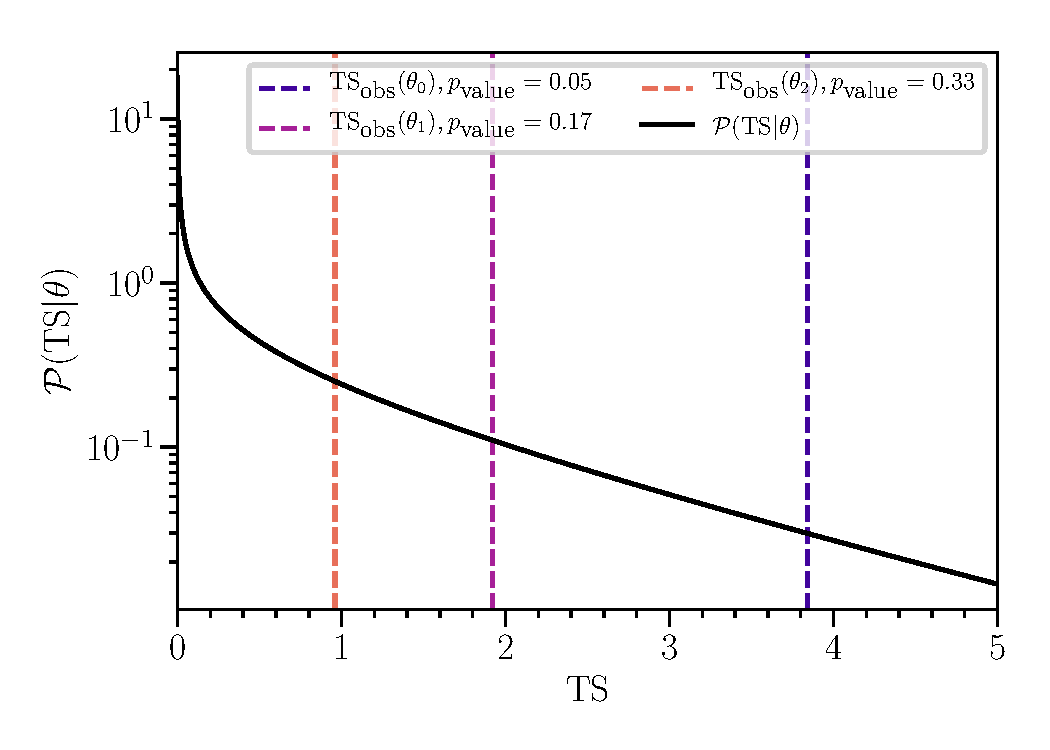
\includegraphics[width=0.8\linewidth]{figures/TS_dist}
	\caption{\textbf{\textit{Test statistic distribution.}} An example of a test statistic distribution.
	Such distributions tend to have the bulk of their mass close to the lower boundary with a long tail.
	Lower values indicate better statistical compatibility with the data.
	}
	\label{fig:TS_dist}
\end{figure}
It is important to note that for the profile likelihood TS and similar statistics a smaller TS value indicates better compatibility with the data.
For this reason many statistical tests are constructed using a single tail significance, by comparing the TS from a single experiment to a background TS distribution and reporting a p-value that is the fraction of the TS distribution greater than the observed TS.

This procedure can be extended to construct intervals by considering the TS distributions of every point in parameter space and comparing to the observed TS function.
Consider the one-dimensional case where there is a TS distribution for each value of the parameter, illustrated in~\reffig{fig:TS_dists_1d}
\begin{figure}
	\centering
	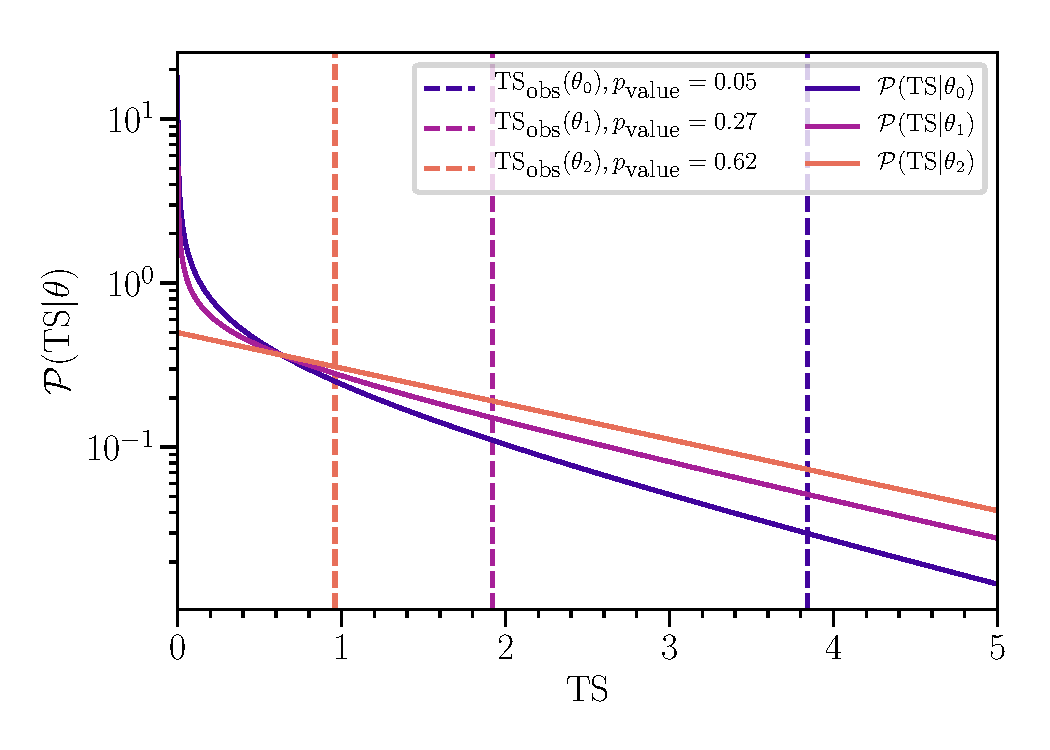
\includegraphics[width=0.8\linewidth]{figures/TS_dists_1d}
	\caption{\textbf{\textit{One-dimensional test-statistic distribution comparison.}} An example of the test statistic distributions as a function of a single parameter.
	}
	\label{fig:TS_dists_1d}
\end{figure}
We can construct an interval that will contain the true value of the parameter a fraction of the time $\alpha$ for repeated experiments.
This interval is the collection of points in the one-dimensional parameter space where the TS at that point is greater than the $\alpha$ quantile of the corresponding TS distribution.
If the TS distribution is the same for all points in parameter space, the interval construction can procedurally be thought of as drawing a horizontal line at the appropriate threshold and only including points that lie below the line.
Varying TS distributions modify this procedure to the comparison of two curves.
This procedure is not limited to one-dimension but can be extended to an arbitrary number of parameters of interest to construct n-dimensional regions with the same properties.

There is however an important caveat to this construction that appears when we consider nuisance parameters.
In order for the intervals to have the desired properties, the observed TS must be greater than the threshold for all possible values of the nuisance parameters.
This ultimatum presents several challenges.
Nuisance parameters can often have a broad or even unbounded range of allowed values, meaning if the effect of nuisance parameters does not taper off at the extrema then almost all intervals are guaranteed to be empty.
From a practical standpoint, computing the TS distributions for many points in parameter space is often done via Monte-Carlo and is computationally expensive.
Adding additional dimensions to the parameter space for which we must compute TS distributions exponentially increases the computation time.

To combat these issues we can limit our interval construction to be valid for values of the nuisance parameters that are ``reasonable''.
There are several methods for doing this, but we can split them into two categories: pure frequentist, and frequentist-Bayesian hybrid.
In the pure frequentist approaches we can either choose a single value of the nuisance parameters, or work with a limited range of the nuisance parameter values.
For the single value approach either nominal values are chosen before looking at the data, or estimators of the nuisance parameters are used to choose their values.
This approach benefits from simplicity, but fails if the test-statistic distributions vary rapidly with changes to the nuisance parameters for values that we might consider ``reasonable''.
A more expensive but robust approach is to explore the behavior of TS distributions for a limited range of the nuisance parameter values, which can be chosen {\it a priori} or from data-based bounds on the nuisance parameters.
If we are willing to consider a hybrid approach, then some more pragmatic options are available.

Although Bayesian methods could be used to choose a single point in parameter space from which to generate the TS distributions, the more interesting application is one that uses a distribution in parameter space.
In Bayesian statistics we can directly assign a probability density to the points in parameter space, either based on our prior information, or directly informed by the posterior distribution, from this extended perspective the probability of certain nuisance parameter values is of interest when considering the frequency of TS values for different parameters of interest.
The prior case is simple in that we sample the from the nuisance parameter priors when generating the TS distribution which allows us to account for variability introduced by the nuisance parameters without relying on hard cutoffs or biasing our inferences with parameter values that are unrealistic.
This prior based technique is well motivated if the priors are derived from external observations, however in the case where nuisance parameters have broad or ``uninformative'' priors this motivation and benefit may break down.
In some cases we expect nuisance parameters to be heavily constrained by the same data sample used to investigate the parameters of interest, so a different approach is merited.
The alternative is to use the posterior distribution to construct our nuisance parameter p.d.f.
Ideally a posterior distribution would be computed for each point in the parameters of interest space by fixing those parameters of interest.
In this way the nuisance parameter posterior used for sampling depends on the point in parameter space we are examining.

With the possible solutions available, we can now look at the problem of limited simulation size when generating test statistic distributions.
As explored in~\refsec{sec:limited_simulation} for binned Poisson likelihood problems, the real expectation in data or simulation for the number of events in a bin is not a known quantity.
Because the real expectations are not known, it is impossible to exactly model the distribution of TS that are expected for a particular point in the parameter space.
However, as~\refsec{sec:limited_simulation} also explored, limited simulation can be modeled with nuisance parameters so the techniques discussed above can be applied directly to the problem.
The ``single point in parameter space'' approach fails to address the additional uncertainty present in this case.
Allowing for unbounded variation of the bin expectations fails as it is guaranteed to produce empty intervals.
Bounding of the bin expectations within a reasonable range provides manageable intervals, but the dimensionality of the problem makes this computationally unfeasible beyond a handful of bins.
Unfortunately this excludes all the ``classic'' frequentist solutions to this problem.
The hybrid Bayesian-frequentist methods in this case provide a tractable solution that accounts for the additional uncertainty.
We can make use of the treatment described in~\refsec{sec:effective}, where the bin expectation is derived to be gamma distributed, and the expected number of data events modeled to be Poisson distributed once this expectation is known.
Practically this can be achieved by sampling data events from $\mcl$, or through a two step process where the expectation is sampled from a gamma distribution $\gprob(\lambda;\agpar, \bgpar)$ where $\agpar = \frac{\mu^2}{\sigma^2}+1~\textmd{and}~\bgpar=\frac{\mu}{\sigma^2}$, and the data events are sampled from a Poisson distribution $\frac{\lambda^{k}e^{-\lambda}}{k!}$.
It is important to note that this procedure only applies to variations in the data and should not be used to vary simulation expectations.
This is because the TS distribution is intended to model variations in the data, whereas the simulation used for analysis is fixed.
Combined with a similar hybrid treatment for other nuisance parameters, this provides a more complete accounting of the uncertainties given the available modeling.
\endgroup

\section{Dealing with limited simulation samples\label{sec:limited_simulation}}
The contents of this section is reproduced here with minor modifications from a collaborative work with Carlos A. Argüelles, and Tianlu Yuan~\cite{Arguelles:2019izp}.

\begingroup
\graphicspath{{results/mcllh_paper/}}
\chapter{Introduction}


\endgroup

\subsection{The Poisson likelihood and previous work\label{sec:mc_intro}}
\begingroup
\graphicspath{{results/mcllh_paper/}}
\input{results/mcllh_paper/sections/previous_work/poisson}
\endgroup

\subsubsection{The Barlow-Beeston likelihood}
\begingroup
\graphicspath{{results/mcllh_paper/}}
\input{results/mcllh_paper/sections/previous_work/bb}
\endgroup

\subsubsection{Uncertainties in the large-sample limit}
\begingroup
\graphicspath{{results/mcllh_paper/}}
\input{results/mcllh_paper/sections/previous_work/chi2}
\endgroup

\subsection{Generalization of the Poisson likelihood\label{sec:generalization_poisson}}
\begingroup
\graphicspath{{results/mcllh_paper/}}
\input{results/mcllh_paper/sections/generalized_poisson/generalized_poisson}
\endgroup

\subsubsection{Derivation of $\like (\lambda|\vecw(\vectheta))$ for identical weights\label{sec:constructing}}
\begingroup
\graphicspath{{results/mcllh_paper/}}
\input{results/mcllh_paper/sections/generalized_poisson/identical_weights}
\endgroup

\subsubsection{Extension to arbitrary weights\label{sec:extending}}
\begingroup
\graphicspath{{results/mcllh_paper/}}
\input{results/mcllh_paper/sections/generalized_poisson/arbitrary_weights}
\endgroup

\subsubsection{The effective likelihood\label{sec:effective}}
\begingroup
\graphicspath{{results/mcllh_paper/}}
\input{results/mcllh_paper/sections/generalized_poisson/effective_likelihood}
\endgroup

\subsubsection{A family of likelihoods\label{sec:priors}}
\begingroup
\graphicspath{{results/mcllh_paper/}}
\input{results/mcllh_paper/sections/generalized_poisson/family}
\endgroup

\subsubsection{Convergence of the effective likelihood\label{sec:llhconvergence}}
\begingroup
\graphicspath{{results/mcllh_paper/}}
\input{results/mcllh_paper/sections/generalized_poisson/convergence}
\endgroup

\subsubsection{Behavior of the effective likelihood\label{sec:llhbehavior}}
\begingroup
\graphicspath{{results/mcllh_paper/}}
\input{results/mcllh_paper/sections/generalized_poisson/behavior}
\endgroup

\subsection{Example and performance\label{sec:example}}
\begingroup
\graphicspath{{results/mcllh_paper/}}
\input{results/mcllh_paper/sections/example/example}
\endgroup

\subsubsection{Point estimation\label{sec:pointestimation}}
\begingroup
\graphicspath{{results/mcllh_paper/}}
\input{results/mcllh_paper/sections/example/point_estimation}
\endgroup

\subsubsection{Coverage\label{sec:coverage}}
\begingroup
\graphicspath{{results/mcllh_paper/}}
\input{results/mcllh_paper/sections/example/coverage}
\endgroup

\subsubsection{Posterior distributions\label{sec:posterior}}
\begingroup
\graphicspath{{results/mcllh_paper/}}
\input{results/mcllh_paper/sections/example/posterior}
\endgroup

\subsubsection{Performance\label{sec:performance}}
\begingroup
\graphicspath{{results/mcllh_paper/}}
\input{results/mcllh_paper/sections/example/performance}
\endgroup

\subsection{Conclusion\label{sec:llhconclusion}}
\begingroup
\graphicspath{{results/mcllh_paper/}}
\input{results/mcllh_paper/sections/conclusion}
\endgroup

\subsection{Summary of likelihood formulas\label{sec:llhtable}}
\begingroup
\graphicspath{{results/mcllh_paper/}}
\input{results/mcllh_paper/appendices/formulas}
\endgroup
\FloatBarrier
\section{Frequentist confidence intervals with nuisance parameters and limited simulation}\label{sec:low_stats_confidence_intervals}

Frequentist and Bayesian techniques deal with different two different kinds of probability.
In frequentist statistics, the relevant probability is the frequency of the outcome of a repeatable experiment.
Under this framework the important concepts are parameter estimation, confidence intervals, and statistical tests.
In Bayesian statistics, the relevant probabilities come from the application of Bayes theorem which means we can define the probability density of parameters.
This definition of the parameter p.d.f. is applicable to the same problems parameter estimation, interval construction, and statistical tests but comes at the cost of defining ``prior belief'' about parameters.

In this section we will ignore the problem of statistical tests, instead focusing on the common features that underpin parameter estimation and interval construction.
Generally in parameter estimation and interval construction there are two sets of parameters, parameters of interest $\vec\theta$ and nuisance parameters $\vec\eta$.
Fundamentally there is no distinction between these two kinds of parameters.
The difference is only in which parameters we want to infer information about.

For both parameter estimation and interval construction the likelihood function is central.
The likelihood function reflects the plausibility of model parameters given observed data and is defined as $\like(\vec\theta, \vec\eta|\textrm{data}) = p(\textrm{data}|\vec\theta, \vec\eta)$.
Where $p(\textrm{data}|\vec\theta, \vec\eta)$ is the probability of the data given the model parameters.
A useful technique to eliminate nuisance parameters is the profile likelihood technique.
Dropping the explicit notational dependence on data, the profile likelihood function is defined as
\begin{linenomath*}
	\begin{equation}
	\tilde{\like}^\texttt{profile}(\vec\theta) = \max_{\vec\eta} \like(\vec\theta,\vec\eta),
	\label{eq:likelihood_profile}
	\end{equation}
\end{linenomath*}
where often the negative log of the function is maximized in place of the function for computational reasons.
The profile likelihood is then only a function of the parameters of interest.
Parameter estimation can be performed by maximizing the profile likelihood to obtain the ``best-fit'' parameters
\begin{linenomath*}
	\begin{equation}
	\hat{\vec\theta} = \argmax_{\vec\theta} \tilde{\like}^\texttt{profile}(\vec\theta).
	\label{eq:best_fit}
	\end{equation}
\end{linenomath*}
This best-fit point in the parameter space is a derived property of the likelihood function.
However, the same procedure can be performed with other functions to the same effect.
In general a minimization procedure is used, and we refer to these functions as ``test-statistics'' (TS).
A particularly useful TS is derived directly from the profile likelihood technique,
\begin{linenomath*}
	\begin{equation}
	\TS(\vec\theta) = -2\log{\left(\frac{\tilde{\like}^\texttt{profile}(\vec\theta)}{\tilde{\like}^\texttt{profile}(\hat{\vec\theta})}\right)}.
	\end{equation}
\end{linenomath*}
Using this TS to perform parameter estimation through minimization is mathematically equivalent to maximizing the likelihood, however, this form will prove to be uniquely useful for interval construction.

Since frequentist statistics deals with the frequency of outcomes from repeated experiments we can use the TS that results from repeated experiments to construct probabilities.
Consider for a moment a single point in the parameter space $\vec\theta_0$.
At this point in the parameter space there is a distribution of data that can be observed, and therefore a distribution of TS functions.
Instead of considering the distribution of TS functions originating from this point, we can simplify the picture by looking at the TS function only evaluated at this point $\TS(\vec\theta_0)$.
This gives us a distribution of TS values for this point in the parameter space that may look like~\reffig{fig:TS_dist}.
\begin{figure}
	\centering
	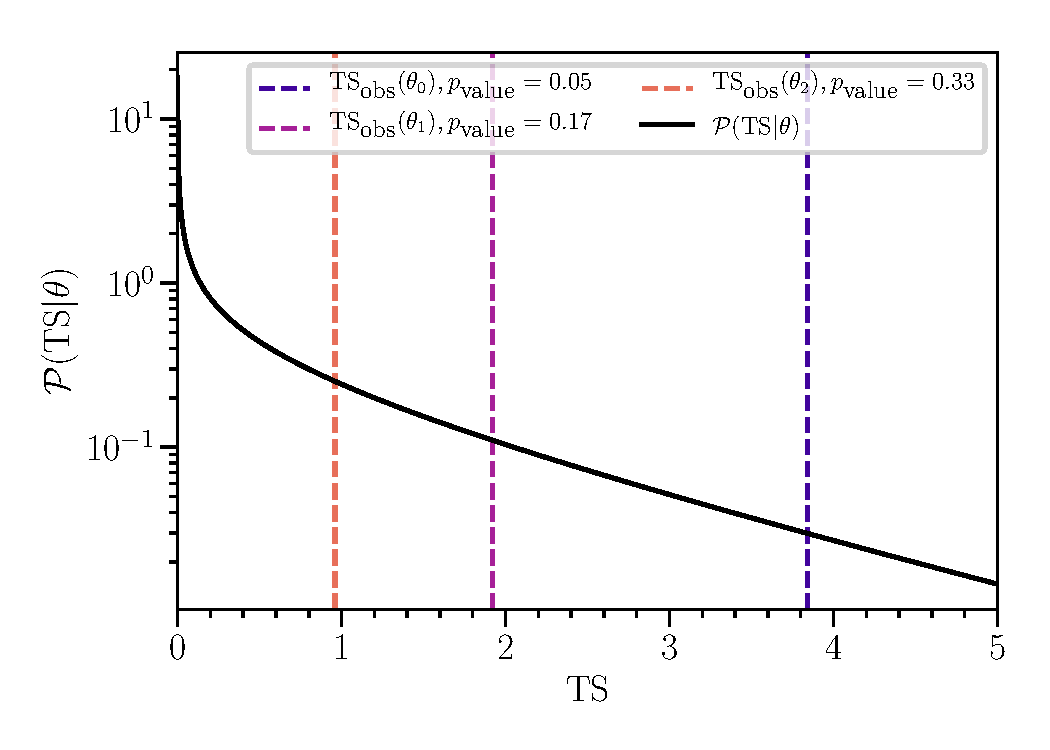
\includegraphics[width=0.8\linewidth]{figures/TS_dist}
	\caption{\textbf{\textit{Test statistic distribution.}} An example of a test statistic distribution.
	Such distributions tend to have the bulk of their mass close to the lower boundary with a long tail.
	Lower values indicate better statistical compatibility with the data.
	}
	\label{fig:TS_dist}
\end{figure}
It is important to note that for the profile likelihood TS and similar statistics a smaller TS value indicates better compatibility with the data.
For this reason many statistical tests are constructed using a single tail significance, by comparing the TS from a single experiment to a background TS distribution and reporting a p-value that is the fraction of the TS distribution greater than the observed TS.

This procedure can be extended to construct intervals by considering the TS distributions of every point in parameter space and comparing to the observed TS function.
Consider the one-dimensional case where there is a TS distribution for each value of the parameter, illustrated in~\reffig{fig:TS_dists_1d}
\begin{figure}
	\centering
	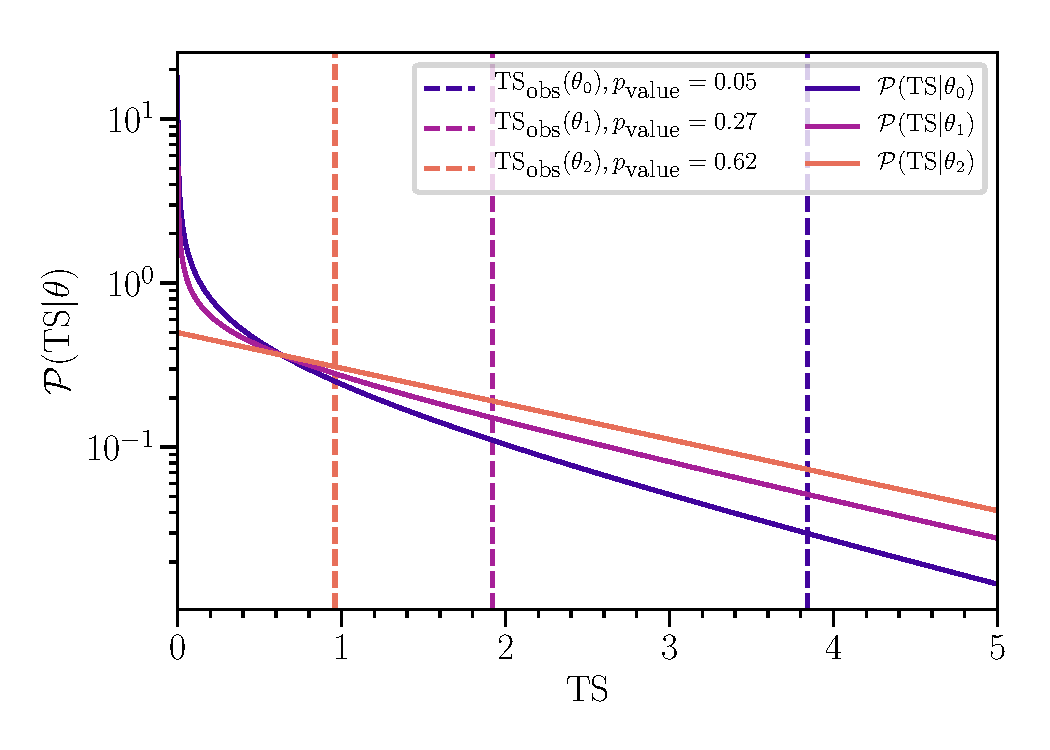
\includegraphics[width=0.8\linewidth]{figures/TS_dists_1d}
	\caption{\textbf{\textit{One-dimensional test-statistic distribution comparison.}} An example of the test statistic distributions as a function of a single parameter.
	}
	\label{fig:TS_dists_1d}
\end{figure}
We can construct an interval that will contain the true value of the parameter a fraction of the time $\alpha$ for repeated experiments.
This interval is the collection of points in the one-dimensional parameter space where the TS at that point is greater than the $\alpha$ quantile of the corresponding TS distribution.
If the TS distribution is the same for all points in parameter space, the interval construction can procedurally be thought of as drawing a horizontal line at the appropriate threshold and only including points that lie below the line.
Varying TS distributions modify this procedure to the comparison of two curves.
This procedure is not limited to one-dimension but can be extended to an arbitrary number of parameters of interest to construct n-dimensional regions with the same properties.

There is however an important caveat to this construction that appears when we consider nuisance parameters.
In order for the intervals to have the desired properties, the observed TS must be greater than the threshold for all possible values of the nuisance parameters.
This ultimatum presents several challenges.
Nuisance parameters can often have a broad or even unbounded range of allowed values, meaning if the effect of nuisance parameters does not taper off at the extrema then almost all intervals are guaranteed to be empty.
From a practical standpoint, computing the TS distributions for many points in parameter space is often done via Monte-Carlo and is computationally expensive.
Adding additional dimensions to the parameter space for which we must compute TS distributions exponentially increases the computation time.

To combat these issues we can limit our interval construction to be valid for values of the nuisance parameters that are ``reasonable''.
There are several methods for doing this, but we can split them into two categories: pure frequentist, and frequentist-Bayesian hybrid.
In the pure frequentist approaches we can either choose a single value of the nuisance parameters, or work with a limited range of the nuisance parameter values.
For the single value approach either nominal values are chosen before looking at the data, or estimators of the nuisance parameters are used to choose their values.
This approach benefits from simplicity, but fails if the test-statistic distributions vary rapidly with changes to the nuisance parameters for values that we might consider ``reasonable''.
A more expensive but robust approach is to explore the behavior of TS distributions for a limited range of the nuisance parameter values, which can be chosen {\it a priori} or from data-based bounds on the nuisance parameters.
If we are willing to consider a hybrid approach, then some more pragmatic options are available.

Although Bayesian methods could be used to choose a single point in parameter space from which to generate the TS distributions, the more interesting application is one that uses a distribution in parameter space.
In Bayesian statistics we can directly assign a probability density to the points in parameter space, either based on our prior information, or directly informed by the posterior distribution, from this extended perspective the probability of certain nuisance parameter values is of interest when considering the frequency of TS values for different parameters of interest.
The prior case is simple in that we sample the from the nuisance parameter priors when generating the TS distribution which allows us to account for variability introduced by the nuisance parameters without relying on hard cutoffs or biasing our inferences with parameter values that are unrealistic.
This prior based technique is well motivated if the priors are derived from external observations, however in the case where nuisance parameters have broad or ``uninformative'' priors this motivation and benefit may break down.
In some cases we expect nuisance parameters to be heavily constrained by the same data sample used to investigate the parameters of interest, so a different approach is merited.
The alternative is to use the posterior distribution to construct our nuisance parameter p.d.f.
Ideally a posterior distribution would be computed for each point in the parameters of interest space by fixing those parameters of interest.
In this way the nuisance parameter posterior used for sampling depends on the point in parameter space we are examining.

With the possible solutions available, we can now look at the problem of limited simulation size when generating test statistic distributions.
As explored in~\refsec{sec:limited_simulation} for binned Poisson likelihood problems, the real expectation in data or simulation for the number of events in a bin is not a known quantity.
Because the real expectations are not known, it is impossible to exactly model the distribution of TS that are expected for a particular point in the parameter space.
However, as~\refsec{sec:limited_simulation} also explored, limited simulation can be modeled with nuisance parameters so the techniques discussed above can be applied directly to the problem.
The ``single point in parameter space'' approach fails to address the additional uncertainty present in this case.
Allowing for unbounded variation of the bin expectations fails as it is guaranteed to produce empty intervals.
Bounding of the bin expectations within a reasonable range provides manageable intervals, but the dimensionality of the problem makes this computationally unfeasible beyond a handful of bins.
Unfortunately this excludes all the ``classic'' frequentist solutions to this problem.
The hybrid Bayesian-frequentist methods in this case provide a tractable solution that accounts for the additional uncertainty.
We can make use of the treatment described in~\refsec{sec:effective}, where the bin expectation is derived to be gamma distributed, and the expected number of data events modeled to be Poisson distributed once this expectation is known.
Practically this can be achieved by sampling data events from $\mcl$, or through a two step process where the expectation is sampled from a gamma distribution $\gprob(\lambda;\agpar, \bgpar)$ where $\agpar = \frac{\mu^2}{\sigma^2}+1~\textmd{and}~\bgpar=\frac{\mu}{\sigma^2}$, and the data events are sampled from a Poisson distribution $\frac{\lambda^{k}e^{-\lambda}}{k!}$.
It is important to note that this procedure only applies to variations in the data and should not be used to vary simulation expectations.
This is because the TS distribution is intended to model variations in the data, whereas the simulation used for analysis is fixed.
Combined with a similar hybrid treatment for other nuisance parameters, this provides a more complete accounting of the uncertainties given the available modeling.
\endgroup

\chapter{Event reconstruction and simulation}\label{chapter:reconstruction}
\begingroup
\graphicspath{{results/HESE_Final_Paper/}}
\chapter{Event reconstruction and simulation}\label{chapter:reconstruction}
\begingroup
\graphicspath{{results/HESE_Final_Paper/}}
\chapter{Event reconstruction and simulation}\label{chapter:reconstruction}
\begingroup
\graphicspath{{results/HESE_Final_Paper/}}
\input{results/HESE_Final_Paper/sections/reconstruction}
\endgroup
\endgroup
\endgroup
\chapter{Estimation of backgrounds}\label{chapter:backgrounds}\label{sec:background_estimation}

In the search for astrophysical neutrinos, the predominant backgrounds are from atmospheric neutrinos and atmospheric muons.
Single atmospheric neutrinos are able to produce the same event signatures as astrophysical neutrinos because they are not fundamentally different than astrophysical neutrinos.
Atmospheric neutrinos can only be distinguished from their astrophysical counterparts by examining the population properties, or by the fact that muons produced in the same air shower can also reach the detector simultaneously.
Muons from cosmic ray air showers differ from neutrinos in their event signature as they always produce light while entering the detector, while neutrinos can interact within the detector volume before any light is produced near the edge of the detector.
Muons can also only be observed up to a certain amount of overburden, beyond which they will lose their energy and decay before reaching the detector.
This means the up-going observation region is free from atmospheric muons.
The task in this section is to model these backgrounds and estimate the contribution of them in the final event selection.
For atmospheric neutrinos the initial flux is modeled with existing calculations.
However the estimation of this background in the sample must also account for the fraction of atmospheric neutrinos rejected because of muons present in the air shower.
Section~\ref{sec:nu_fluxes} details how the atmospheric neutrino flux is modeled, while \refsec{sec:passingfractions} explores a new calculation of the atmospheric neutrino passing fractions and explores the many factors that may affect this calculation, and \refsec{sec:hese_passingfractions} applies this calculation to the HESE selection.
The passing fraction calculation described in this chapter was developed in collaboration with Carlos A. Argüelles, Sergio Palomares-Ruiz, Logan Wille, and Tianlu Yuan~\cite{Arguelles:2018awr}.
Finally, \refsec{sec:muon_background} explores the contribution of lone muons to the sample.

\section{Neutrino background estimation}
\subsection{Neutrino fluxes\label{sec:nu_fluxes}}

Atmospheric neutrinos are predominantly produced by the decay of pions and kaons, which we shall call the ``conventional'' component.
At energies above $\SI{1}\TeV$ the spectrum of the conventional component is softer than the incident cosmic-ray spectrum by one unit in the spectral index, due to the interactions of these mesons in the atmosphere.
The conventional neutrino flux is largest at the horizon, $\cos\theta_z=0$~\cite{Gaisser:2002jj,Barr:2004br,Honda:2006qj,Petrova:2012qf} because the larger path length in the thin atmosphere increases the proportion of pions that can decay before interacting.
To model the conventional neutrino flux, we use a parameterization of the Honda {\it{}et al.} 2006 flux calculation~\cite{Honda:2006qj} given in~\cite{Montaruli:2011as} which at the highest energies uses the analytic parameterization of the neutrino flux in~\cite{Gaisser:2002jj}.
This calculation is tuned to match observations of atmospheric muons, which remain difficult to predict from first principles.

A sub-leading -- yet unobserved -- contribution due to charmed hadron decays is expected to be important above $\sim\SI{100}\TeV$~\cite{Bhattacharya:2015jpa}.
Since the charmed hadrons decay promptly and do not interact in the atmosphere at the energies relevant for this analysis, we call this the ``prompt'' component.
Thus, at these energies, the prompt component has a spectral index close to the incident cosmic-ray spectrum.
The prompt flux is also constant with respect to the cosine of the zenith angle, as the short decay time of the charmed hadrons removes the effect of different path lengths through the atmosphere.
To model the prompt neutrino flux at Earth's surface, we use the flux computed in~\cite{Bhattacharya:2015jpa}.

The angular and energy distribution of the initial atmospheric neutrino flux is modified with respect to the flux at Earth's surface because of absorption of high-energy neutrinos in the Earth.
We account for this using a dedicated Monte Carlo, similar to the one described in~\cite{Gazizov:2004va}, that simulates the propagation of neutrinos in the Earth.
In this Monte Carlo we use the isoscalar neutrino cross sections given in~\cite{CooperSarkar:2011pa} for the neutrino-nucleon interactions, and the Earth density model described in~\cite{Dziewonski:1981xy}.
Neutrino-electron scattering can be safely neglected except for resonant-W production~\cite{Glashow:1960zz} which we include.
We ignore the uncertainties on the Earth opacity as they are known to be sub-leading in this energy range~\cite{Gandhi:1995tf,CooperSarkar:2011pa,Vincent:2017svp}.

Modeling the atmospheric neutrino flux with these two components does not account for the contribution of $K_s$~\cite{Gaisser:2014pda}, which is $\sim \SI{10}\percent$ at $\SI{100}\TeV$ and well-within our uncertainties.
In order to account for uncertainties in the cosmic-ray flux~\cite{Dembinski:2017zsh} and hadronic interactions~\cite{Fedynitch:2012fs} we parameterize the atmospheric neutrino flux as
\noindent
\begin{linenomath*}
	\begin{equation}
	\begin{split}
	\phi_\nu^{\rm{atm}} =& \Phi_{conv} \bigg(\phi^\pi_\nu + R_{K/\pi} \phi^K_\nu\bigg) {\bigg(\frac{E_\nu}{E_0^c} \bigg)}^{-\Delta \gamma_{CR}} \\ &+ \Phi_{prompt} \phi^p_\nu {\bigg(\frac{E_\nu}{E_0^p} \bigg)}^{-\Delta \gamma_{CR}},
	\end{split}
	\label{eq:atm_flux_equation}
	\end{equation}
\end{linenomath*}
where $\phi^\pi_\nu$, $\phi^K_\nu$, and $\phi^p_\nu$ are the conventional pion, kaon, and prompt atmospheric neutrino fluxes at a neutrino energy $E_\nu$ respectively.

The parameters $\convnorm$ and $\promptnorm$ are normalizations for the conventional and prompt normalizations respectively; $\pik$ allows us to modify the relative kaon to pion contributions; and the $\crdeltagamma$ parameter allows for hardening or softening of the atmospheric neutrino component to account for uncertainties in the cosmic-ray flux slope.
These parameters are incorporated into the analysis as nuisance parameters with priors as summarized in \reftab{tbl:priors}.
This analysis refrains from directly using prior information from other IceCube neutrino studies in order to provide results independent from other neutrino samples.

The conventional normalization prior is motivated by studies of the total uncertainty due to cosmic-ray and high-energy hadronic processes~\cite{Fedynitch:2012fs}; it is chosen to be Gaussian for simplicity with an expectation centered on the baseline flux model and appropriate variance.
The standard deviation of the Gaussian prior on the cosmic-ray slope parameter has been chosen to be $0.05$ in order to accommodate values measured at intermediate~\cite{Karelin:2011zz} and high~\cite{Bartoli:2015fhw,Yoon:2017qjx,Alfaro:2017cwx} energies.
The uncertainty on corrections to the ratios of neutrinos-to-anti-neutrinos ($\atmonunubar$) and kaon-pion yields ($\pik$) were estimated by comparing the expectation of different atmospheric neutrino calculations and a Gaussian prior width was chosen that encompasses their predictions.
Details regarding these corrections and the different atmospheric neutrino flux calculations can be found in~\cite{CollinFluxes,Jones:2015bya}.
Finally, the parameters $E_0^c=\SI{2020}\GeV$ and $E_0^p=\SI{7887}\GeV$ are points of fixed differential flux for the conventional and prompt components.

This simple parameterzation of the atmospheric neutrino flux and its uncertainties is chosen because it models the primary systematic effects of physical uncertainties that are observable with this sample.
Of course this neglects other physical uncertainties, such as those regarding the hadronic interactions in cosmic ray air showers and the composition of the cosmic ray particles.
But, these effects do not produce modifications to the observations that can be statistically discerned with the amount of data available.
Later it will be shown that even the modeled systematic uncertainties have a small effect on astrophysical measurements compared to the statistical uncertainties.

The above description models the flux of atmospheric neutrinos, but does not fully encapsulate the detector response to atmospheric neutrinos.
We have so far neglected the effect of accompanying muons on the detector response.
This is discussed at length in \refsec{sec:muon_background}.

\subsection{Atmospheric neutrino passing fractions}
\label{sec:passingfractions}
This discussion and study of atmospheric passing fractions is directly adapted from a collaborative work with Carlos A. Argüelles, Sergio Palomares-Ruiz, Logan Wille, and Tianlu Yuan~\cite{Arguelles:2018awr}.
Figures and equations are reproduced from~\cite{Arguelles:2018awr}, and the text follows the same thread of discussion.

As noted in~\cite{Schonert:2008is}, muons produced in the same air-shower may trigger the detector veto in coincidence with the neutrino interaction.
Dedicated simulations of cosmic ray air showers where neutrino interactions are forced can provide observational predictions for the distribution of these combined muon+neutrino events.
However, available simulation techniques to create these estimates remain prohibitively expensive for the desired accuracy.
Instead, we look to model this effect by computing an average efficiency with respect to the case where no muons reach the detector.
To account for this when weighting the neutrino-only simulation each atmospheric neutrino flux component, $i$, is multiplied by an efficiency.
This efficiency is referred to as the ``atmospheric neutrino passing fraction'', and denoted by $\mathcal{P}^{i,\alpha}_{passing}$, for each neutrino flavor $\alpha$.

The passing fraction depends on the details of air shower development, which includes modeling of the hadronic interaction, and the energy losses of muons in the material between the shower and the detector. 
Air-shower properties are averaged over in this calculation, but the passing fraction is still a probability that is conditional on the neutrino properties.
Of particular interest are the potential systematic dependencies of the passing fraction, which include the cosmic ray spectrum and composition, the hadronic interaction model, muon energy losses, and the atmospheric density model.
The calculation of the passing fraction is designed so that these systematic dependencies may be changed between different alternatives.
Additionally, the detector response enters in only one place in the formalism as a probability of muon rejection.
This allows for simple variation of the detector response modeling in a generic way.
To perform this calculation a framework was developed that leverages the Matrix Cascade Equation (MCEq) package in key portions of the calculation.
Validation of the computed passing fractions is performed against detailed air shower simulations with COsmic Ray SImulations for KAscade (CORSIKA), and excellent agreement is found as a result.

Departure from the lone-neutrino case is based on the coincidence of a muon and neutrino from the same air-shower that occurs in both time and direction.
Thus,
\begin{equation}
\label{eq:preach}
\Prob_{\rm reach}\left(\Emf \, | \, \Emi , \, X_\mu, \right)
\end{equation}
is naturally a key component of the calculation, which describes the probability of a muon with initial energy $\Emi$ and slant depth $X_\mu$ to reach the detector with energy $\Emf$.
As the IceCube detector is deep underground, the contribution to slant depth from the atmosphere is very small compared to that of the Earth, and so can be neglected.
With only the slant depth of the Earth contributing, $X_\mu$ is fully specified by the zenith angle $\theta_z$ in detector coordinates and the depth $d$.
Stochasticity of the muon energy losses is accounted for by the distribution $\Prob_{\rm reach}$, which is computed by tabulating simulations of muons propagated in ice by the software $\MMC$.
Using the conditional probability distribution $\Prob_{\rm reach}$ instead of average muon behavior ensures that contributions from the distribution tails are accounted for.
These contributions from the tails become important for very large slant depths, where muons on average do not reach the detector.
Departure from the neutrino-only case requires both the muon to reach the detector, but also for the muon to trigger a response, in this case for the muon to {\it light} the veto.
The quantity
\begin{equation}
\label{eq:plight}
\Prob_{\rm light}(\Emf,d)
\end{equation}
is the probability that a muon of energy $\Emf$ and depth $d$ at the detector boundary {\it lights} the veto, such that the event is rejected.
In practice, this $\Prob_{\rm light}$ is computed by tabulating detector simulations of atmospheric muons and incorporating the specifics of the event selection.
With both $\Prob_{\rm light}$ and $\Prob_{\rm reach}$ in hand, the probability of detecting an incident muon $\Prob_{\rm det}$ can be computed as 

\begin{equation}
\label{eq:PrPl}
\Prob_{\rm det}\left(\Emi , \, X_\mu(\theta_z, d), d\right) \equiv \int d\Emf \, \Prob_{\rm reach}\left(\Emf \, | \, \Emi , \, X_\mu(\theta_z, d)\right) \, \Prob_{\rm light} (\Emf, d) ~.
\end{equation}

Note that losses also depend on the medium and not only on the slant depth, whose dependence on $\theta_z$ we write explicitly. If the medium surrounding the detector is homogeneous, the dependence on $X_\mu$ can be exchanged for distance without loss of generality.
From here on to simplify the notation, the dependence on $X_\mu$ will be replaced by a dependence on $\theta_z$ and the dependence on $d$ will be neglected.
These dependencies can be added back in at the end of the calculation without any change to the result.

\begin{figure}
	\centering
    \begin{subfigure}{\linewidth}
		\centering
		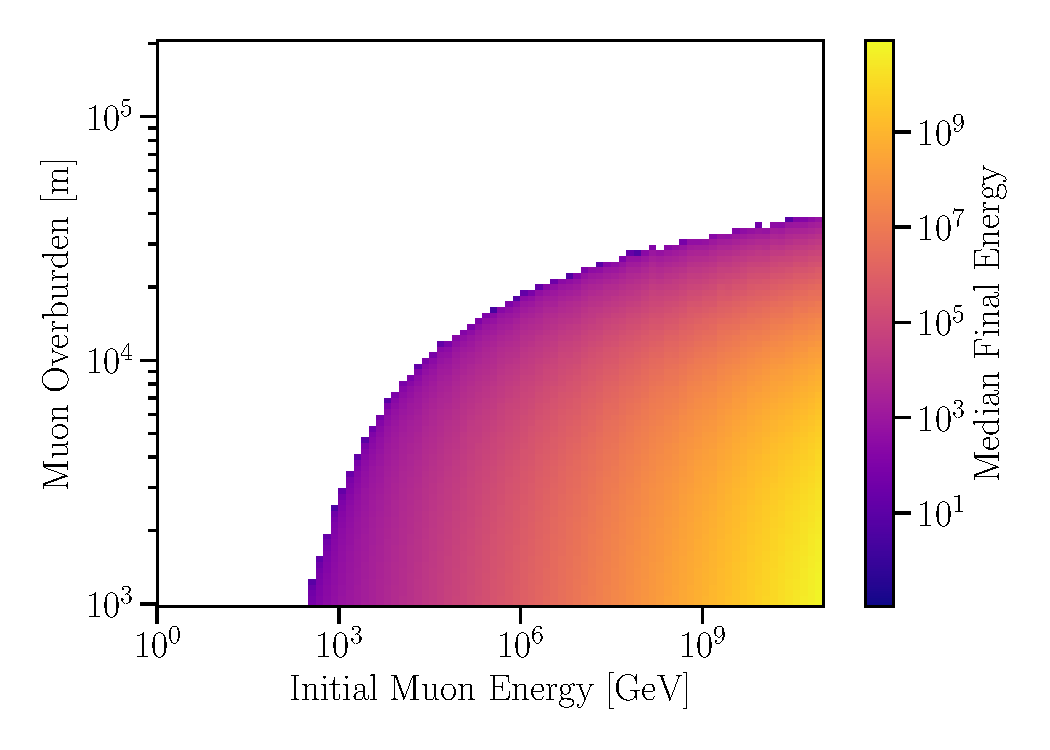
\includegraphics[width=0.8\linewidth]{figures/preach_median}
	\end{subfigure}
	\begin{subfigure}{\linewidth}
		\centering
		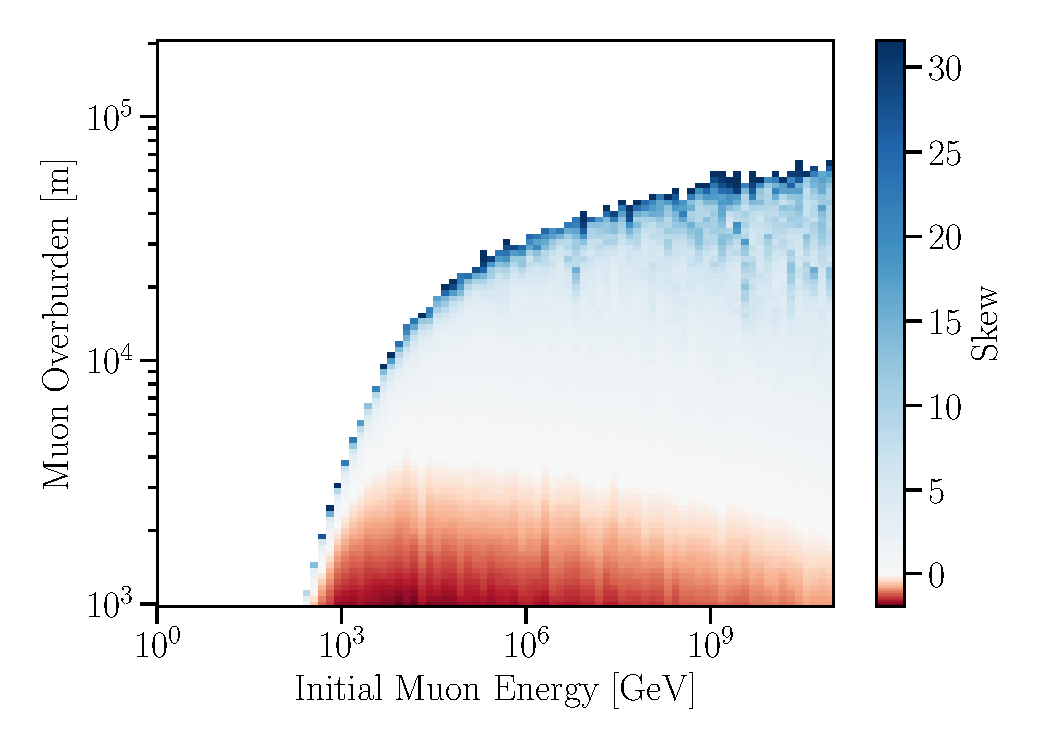
\includegraphics[width=0.8\linewidth]{figures/preach_skew}
	\end{subfigure}
	\caption{\textbf{\textit{Muon Final Energy Statistics.}} Muons propagating in ice were simulated for a wide range of initial energies, and at a set of predefined distances their energy was recorded.
	This results in a distribution of final muon energies for each combination of initial muon energy and overburden.
	These two plots show statistics of these distributions, with the upper plot displaying the median and the lower plot displaying the skew.
	Previous calculations only used the median of these distributions, creating a one-to-one mapping from initial to final muon energy for each overburden or angle as shown in the upper panel.
	However, the large skew of these distributions shows us that the tails become important for large overburdens as the lower panel shows.
	}
	\label{fig:preach_stats}
\end{figure}

For an atmospheric neutrino of known energy and direction the passing fraction is defined as the probability that muons from the same air shower do not trigger the detector veto.
This probability is denoted $\Prob_{\rm pass}$~\cite{Schonert:2008is, Gaisser:2014bja} and can be written as the ratio
\begin{equation}
\Prob_{\rm pass} (E_\nu, \theta_z) = \frac{\phi_\nu^{\rm pass}(E_\nu, \theta_z)}{\phi_\nu(E_\nu, \theta_z)} ~,
\end{equation}
where $E_\nu$ is the neutrino energy, $\theta_z$ is the zenith angle, $\phi_\nu^{\rm pass}$ is the differential flux of atmospheric neutrinos accompanied by muons that are detected, and $\phi_\nu$ is the total differential atmospheric neutrino flux.
In the next sections, passing fractions for electron neutrinos and muon neutrinos are derived.
As tau neutrinos by comparison make up a very small portion of the atmospheric flux, there is no dedicated discussion for this case.
However, the concerns for tau neutrinos are very similar to those of electron neutrinos minus the differences in their production.

\subsubsection{$\nu_e$ passing fraction}
Electron neutrinos (or antineutrinos) are produced alongside a positron (or electron) in the decay of their parent particle, for example $K^+ \rightarrow \pi^0 + e^+ + \nu_e$.
Rarely does an electron neutrino have a sibling muon, as this would involve a lepton flavor violating process.
Instead, muons that accompany electron neutrinos are produced in other branches of the air shower.
Because the different branches of the shower are uncorrelated, to first order the average properties of muons in a prototypical air shower can be used for the passing fraction calculation.
The task in this section is to track the production and propagation of these muons from uncorrelated branches of the shower and compute the flux of neutrinos not vetoed by these uncorrelated muons.
Consider a shower from a single cosmic-ray primary particle of type $A$ with energy $\ECR$.
The average neutrino yield $\frac{dN_{A, \nu}}{dE_\nu}(\ECR, E_\nu, \theta_z)$ from such a shower can be computed with $\MCEq$.
So the atmospheric neutrino flux can be written as 
\begin{equation}
\label{eq:nuphi}
\phi_\nu(E_\nu, \theta_z)  = \sum_A \int d\ECR \, \frac{dN_{A, \nu}}{dE_\nu}(\ECR, E_\nu, \theta_z) \, \phi_A(\ECR)~,
\end{equation}
where $\phi_A(\ECR)$ is the flux of primary cosmic rays of type A.
the passing fraction can be obtained by modifying the integrand of Eq.~\ref{eq:nuphi} so that it is weighted by the Poisson probability $Pzmproto$ of detecting an accompanying muon.
In this way the uncorrelated passing fraction can be written as
\begin{equation}
\label{eq:PuncorGJKvS}
\Prob_{\rm pass}^{\rm uncor, GJKvS}(E_\nu, \theta_z)  =  \frac{1}{\phi_\nu(E_\nu, \theta_z)} \sum_A \int d\ECR \, \frac{dN_{A, \nu}}{dE_\nu}(\ECR, E_\nu, \theta_z) \, \phi_A(\ECR) \, \Pzmproto \left(N_\mu = 0  ; \bar N_{A, \mu}^{\rm GJKvS}(\ECR, \theta_z)\right)~,
\end{equation}
where $\Pzmproto \left(N_\mu = 0  ; \bar N_{A, \mu}^{\rm GJKvS}(\ECR, \theta_z)\right) = \exp{-\bar N_{A, \mu}^{\rm GJKvS}(\ECR, \theta_z)}$,
and  $\bar N_{A, \mu}^{\rm GJKvS}(\ECR, \theta_z)$ is the average number of muons that are detected from an air shower.
This average number of muons is computed using the yield of muons from the air shower $dN_{A, \mu}/d\Emi(\ECR, \Emi)$ and the probability of detecting those muons, such that
\begin{equation}
\label{eq:Nmu}
\bar N_{A, \mu}^{\rm GJKvS}(\ECR,\theta_z) = \int d\Emi \, \frac{dN_{A, \mu}}{d\Emi}(\ECR, \Emi,  \theta_z) \, \Prob_{\rm det}\left(\Emi , \theta_z\right) ~,
\end{equation}
Some terms in the above equations are labeled with ${\rm GJKvS}$ because these quantities are calculated in the same manner as was done in~\cite{Gaisser:2014bja} under certain choices for $\Prob_{\rm det}$.
Namely, when $\Prob_{\rm light}$ is defined as a Heaviside function with a boundary at $\Emf = \SI{1}\TeV$, and $\Prob_{\rm reach}$ is defined as a delta function that matches the initial muon energy to the median final muon energy.

Fig.~\ref{fig:nue_passing-preach-effect} shows the effect of the two muon treatments on the passing fractions as defined in Eq.~\ref{eq:PuncorGUE}.
At the horizon the median approximation overestimates the passing fraction while near the vertical direction it is underestimated.
In the horizontal region, muons with smaller initial energy such that their median range is less than the distance to the detector represent a small but non-negligible fraction of muons that may trigger the detector veto.
Thus, in the median muon treatment the passing fraction is overestimated because of too few muons.
In the vertical region, with less overburden the probability for muon detection rapidly increases to approximately one with initial muon energy, however this turnover is faster with the median treatment than the full treatment.
This means more muons contribute to the calculation in the median case and the passing fraction is underestimated.

\begin{figure}
	\centering
	\subfloat{
		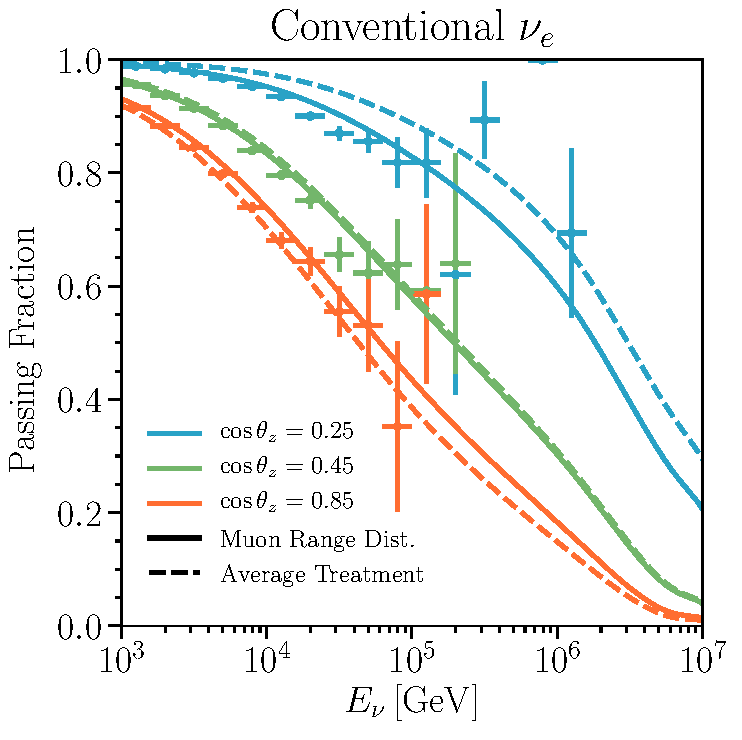
\includegraphics[width=0.45\linewidth]{results/passing_fractions_paper/fig/fig4_nue_conv_murange_vs_avg}
	}
	\subfloat{
		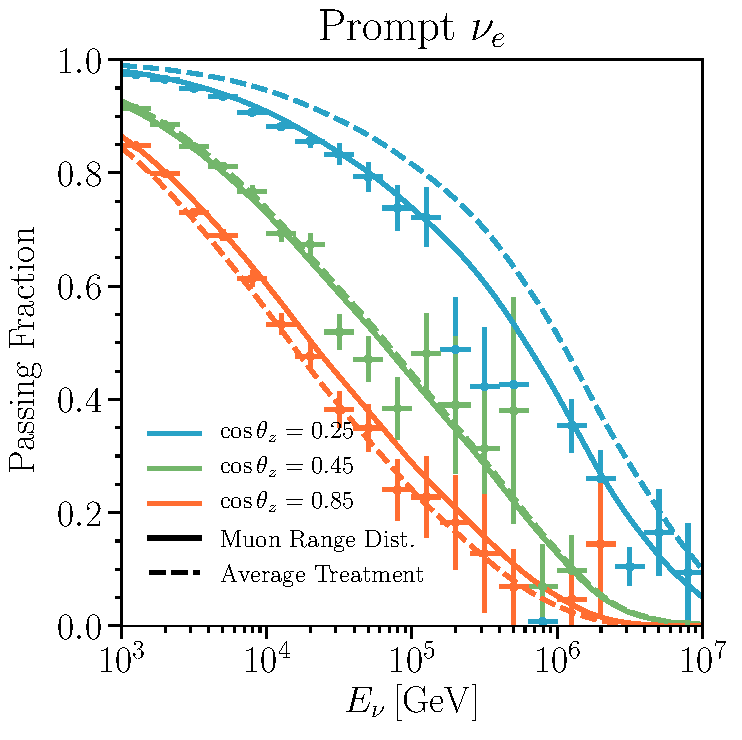
\includegraphics[width=0.45\linewidth]{results/passing_fractions_paper/fig/fig4_nue_prompt_murange_vs_avg}
	}    
	\caption{\textbf{\textit{Passing fractions: effect of the treatment of muon losses in ice.}} Results are shown for three values of $\cos\theta_z$ (from top to bottom): 0.25 (blue), 0.45 (green), and 0.85 (orange); using the full muon range distribution (solid) or the median muon range (dashed). Results from the \CORSIKA{} simulation are shown as crosses, with statistical error bars only. In all cases, the H3a primary cosmic-ray spectrum~\cite{Gaisser:2011cc}, the SIBYLL~2.3 hadronic-interaction model~\cite{Engel:2015dxa, Riehn:2015oba} and the MSIS-90-E atmosphere-density model at the South Pole on July 1, 1997~\cite{Labitzke:1985, Hedin:1991} are used. A depth in ice of $d_{\rm det} = \SI{1.95}\km$ (like the center of IceCube) and a Heaviside $\Prob_{\rm light}(\Emf) = \Theta(\Emf - 1\,{\rm TeV})$ are assumed. \textit{Left panel:} Conventional $\nu_e$ passing fraction. \textit{Right panel:} Prompt $\nu_e$ passing fraction.
	}
	\label{fig:nue_passing-preach-effect}
\end{figure}

In Eq.~\ref{eq:Nmu} the energy available to other branches of the shower to produce uncorrelated muons is over estimated as some energy must be reserved for producing the electron neutrino or rather the branch of the shower that produces the electron neutrino.
A complete modeling of the connection between the three relevant particles (cosmic ray primary, the electron neutrino, and muons) is cumbersome, as it would involve modeling the shower branch producing the electron neutrino in its entirety and then separately modeling the uncorrelated branch.
However, a simple approximation can be made that at least accounts for the energy necessary to produce the electron neutrino.
The electron neutrino must be produced by a parent particle $p$ that has a kinematically allowed energy $E_p$, so the remaining energy is $\ECR-E_p$.
The muon yield is then modeled using the average behavior of a shower that begins with energy $\ECR-E_p$.
Because we are now concerned with the parent particle of the electron neutrino, the slant depth through which this parent particle travels must be considered, as this will affect the probability that it decays to a neutrino instead of interacting.
Now considering the parent particle energy and slant depth, the yield of neutrinos from the air shower can be expanded as
\begin{equation}
\label{eq:Anuyield}
\frac{dN_{A, \nu}}{dE_\nu}(\ECR, E_\nu, \theta_z) = \int dE_p \, \int \frac{dX}{\lambda_p(E_p, X)} \, \frac{dN_{p, \nu}}{dE_\nu}(E_p, E_\nu) \, \frac{dN_{A, p}}{dE_p}(\ECR, E_p, X) ~,
\end{equation}
where $dN_{p, \nu}/dE_\nu(E_p,E_\nu)$ is the spectrum of neutrinos from a parent particle $p$ with energy $E_p$, $dN_{A, p}/dE_p(\ECR,E_p,X)$ is the spectrum of parent particles from the air shower at slant depth $X$, and $dX/{\lambda_p(E_p, X)}$ is the probability of the parent to decay between the slant depth $X$ and $X+dX$.
$\lambda_p(E_p, X)$ is the product of the local density and the parent decay length such that $\lambda_p(E_p, X)=\rho(X) \tau_p E_p/m_p$, where $\rho(X)$ is the local density, $\tau_p$ is the lifetime of the parent, $E_p$ is its energy, and $m_p$ is its mass.
Now Eq.~\ref{eq:PuncorGJKvS} can be rewritten with the above expansion and the simple approximation that accounts for the available energy,
\begin{align}
\label{eq:PuncorGUE}
\Ppuncor (E_\nu, \theta_z) & = \frac{1}{\phi_\nu(E_\nu, \theta_z)} \, \sum_A \sum_{p} \int dE_p \int \frac{dX}{\lambda_p(E_p, X)} \int d\ECR \nonumber \\
& \frac{dN_{p, \nu}}{dE_\nu}(E_p, E_\nu) \, \frac{dN_{A, p}}{dE_p}(\ECR, E_p, X) \, \phi_A(\ECR) \, \Pzmproto \left(N_\mu = 0  ; \bar N_{A, \mu}(\ECR - E_p, \theta_z)\right) ~.
\end{align}
This treatment remains consistent with the calculation of the neutrino flux mentioned earlier, as if the Poisson probability of muon non-detection is removed (i.e. $\Pzmproto=1$) then the passing fraction is $1$ by construction.

The na\"ive approximation of the muon yield using $\ECR$ without the subtraction of $E_p$ tends to underestimate the passing fraction as can bee seen in Fig.~\ref{fig:nue_passing-double-counting}.
This is because the muon yield is larger for showers of greater energy.
Below $\SI{100}\TeV$ the absolute difference between the two methods is below $0.05$, however at higher energies and especially more vertical directions the relative difference becomes more important.

\begin{figure}
	\centering
	\subfloat{
		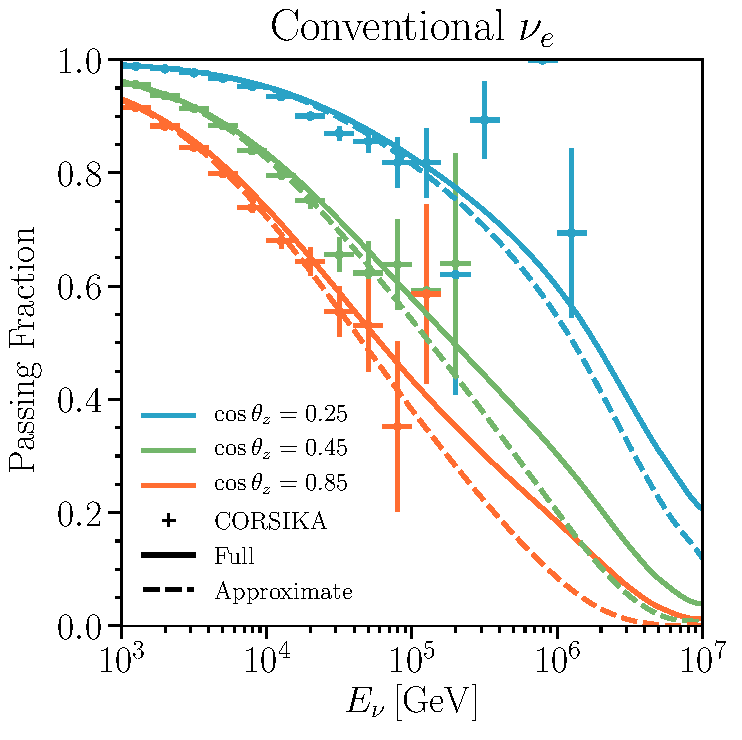
\includegraphics[width=0.45\linewidth]{results/passing_fractions_paper/fig/fig3_b_nue_conventional_unified_versus_factorized_with_corsika_sibyll_23}
	}
	\subfloat{
		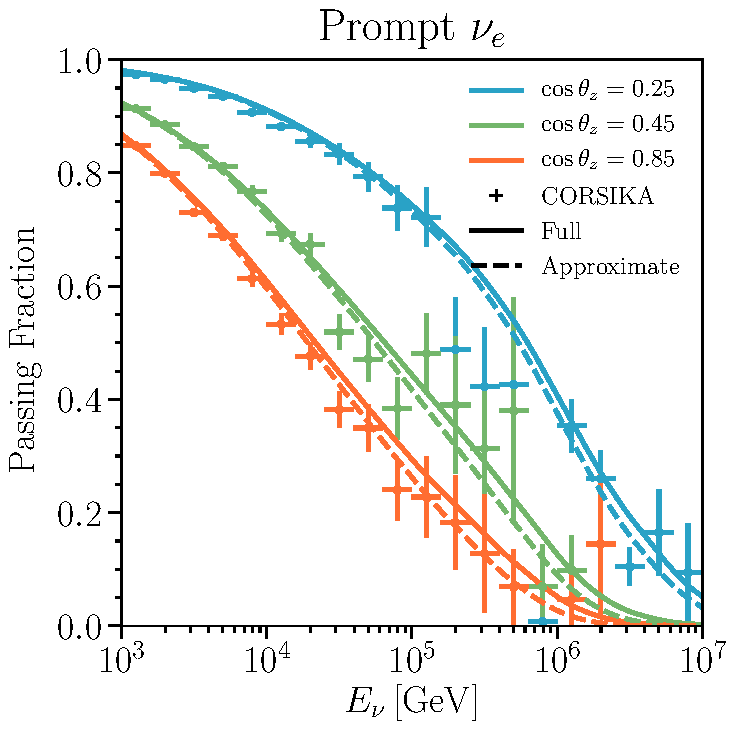
\includegraphics[width=0.45\linewidth]{results/passing_fractions_paper/fig/fig3_a_nue_prompt_unified_versus_factorized_with_corsika_sibyll_23}
	}
	\caption{\textbf{\textit{Passing fractions: effect of approximations on the energy of the shower giving rise to uncorrelated muons.}} Results are shown for three values of $\cos\theta_z$ (from top to bottom): 0.25 (blue), 0.45 (green), and 0.85 (orange); with the approach of this work (solid), Eq.~(\ref{eq:PuncorGUE}), where the energy carried by the neutrino parent is subtracted from the rest of the shower which produces the muons to be triggered (i.e., $\ECR - E_p$), and without this subtraction (dashed), Eq.~(\ref{eq:PuncorGJKvS}), considering the cumulative muon yield from a shower with energy $\ECR$. Results from the \CORSIKA{} simulation are shown as crosses, with statistical error bars only. \textit{Left panel:} Conventional $\nu_e$ passing fraction. \textit{Right panel:} Prompt $\nu_e$ passing fraction.
	}
	\label{fig:nue_passing-double-counting}
\end{figure}

Fig.~\ref{fig:nu-e-neutrino-vs-antineutrino} shows a comparison between this calculation and results from the CORSIKA simulation in addition to the differences between electron neutrino and antineutrino fluxes.
The agreement between simulation and this calculation modeling is excellent for
both neutrinos and antineutrinos.
The conventional electron antineutrino passing fractions are lower than those of conventional electron neutrinos, primarily because positively charged mesons are preferentially produced, leading to a harder spectrum than the negatively charged mesons.
The passing fractions for the prompt flux are almost identical as they are mainly produced from gluon fusion~\cite{Arguelles:2015wba}.

\begin{figure}
	\centering
	\subfloat{
		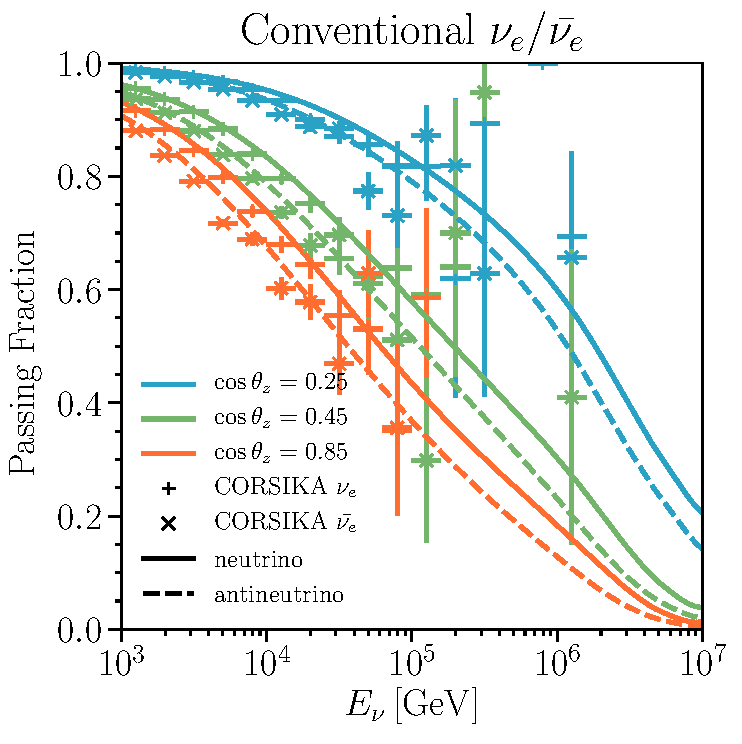
\includegraphics[width=0.45\linewidth]{results/passing_fractions_paper/fig/fig5_nue_conv_nu_vs_nubar}
	}
	\subfloat{
		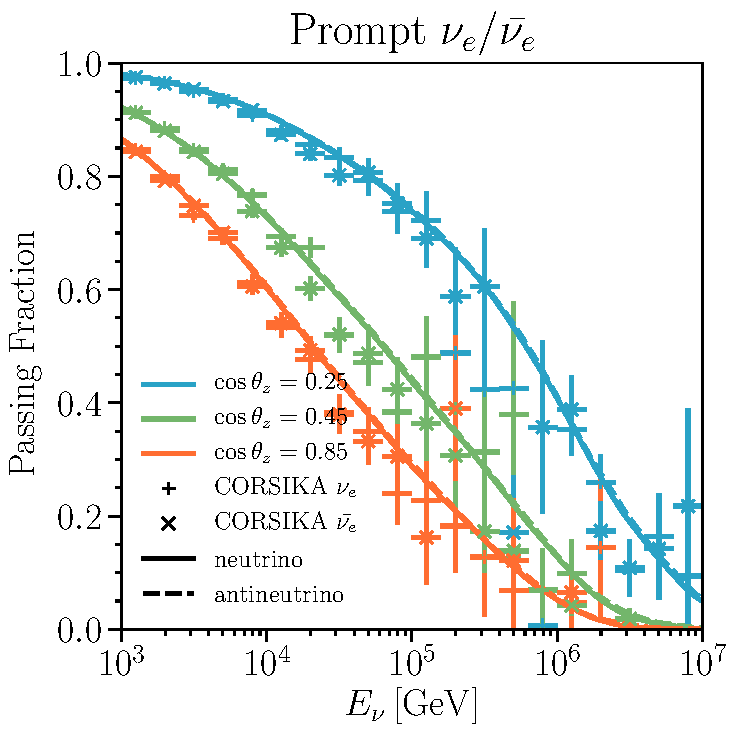
\includegraphics[width=0.45\linewidth]{results/passing_fractions_paper/fig/fig5_nue_prompt_nu_vs_nubar}
	}
	\caption{\textbf{\textit{Passing fractions: neutrinos versus antineutrinos.}} Results are shown for three values of $\cos\theta_z$ (from top to bottom): 0.25 (blue), 0.45 (green), and 0.85 (orange); for neutrinos (solid) and antineutrinos (dashed). Results from the \CORSIKA{} simulation for neutrinos ($+$) and antineutrinos ($\times$) are also shown, with statistical error bars only. In all cases, the H3a primary cosmic-ray spectrum~\cite{Gaisser:2011cc}, the SIBYLL~2.3 hadronic-interaction model~\cite{Engel:2015dxa, Riehn:2015oba} and the MSIS-90-E atmosphere-density model at the South Pole on July 1, 1997~\cite{Labitzke:1985, Hedin:1991} are used, and $d_{\rm det} = 1.95$~km in ice and $\Prob_{\rm light}(\Emf) = \Theta(\Emf - 1\,{\rm TeV})$ are assumed. \textit{Left panel:} Conventional $\nu_e$ passing fraction. \textit{Right panel:} Prompt $\nu_e$ passing fraction. Note that for prompts there are not differences between $\nu_e$ and $\bar\nu_e$.
	}
	\label{fig:nu-e-neutrino-vs-antineutrino}
\end{figure}

\subsubsection{$\nu_\mu$ passing fraction}

Muon neutrinos or antineutrinos produced in hadron decays will always have a sibling muon due to flavor conservation.
This means the passing fraction for muon neutrinos has a correlated component in addition to the uncorrelated component described for electron neutrinos.
This correlated suppression depends entirely on the behavior of the sibling muon, which itself can be described as a function of the muon direction and initial energy.
The task in this section is to now track the sibling muons produced along with the neutrino and compute the flux of neutrinos not vetoed by this muon.
Additionally, the treatment of correlated and uncorrelated muons can be unified, which we also explore.
For two body decays, there is a direct relation between the energy of the parent particle, muon, and neutrino: $\Emi = E_p - E_\nu$.
This relation gives a delta function for the muon energy spectrum $dN_{p,\mu}^{\rm 2-body}/d\Emi (E_p,E_\mu,\Emi)=\delta(\Emi-E_p+E_\nu)$.
However, the two-body approximation is not appropriate for the calculation of the passing fractions for the prompt fluxes, as neutrinos are mainly produced by the decays of $D^{\pm}$, $D^0$, $\bar{D}^0$, $\Lambda_c^+$, and $D_s^{\pm}$~\cite{Fedynitch:2015zma}.
Treatment of $n$-body decays requires evaluating the muon distributions from the decays of these particles and using Eq.~(\ref{eq:pnomusib}).
In this work, $dN_{p, \mu}/d\Emi$ was generated for $K^0_L$, $D^+$, $D^0$, and $D^+_s$.\footnote{The decay distributions for their antiparticles are identical.}
For general $n$-body decays the probability of not detecting this sibling muon is a function of the energy spectrum and can be written as
\begin{equation}
\label{eq:pnomusib}
\Pzmsib \left(\theta_z|E_p, E_\nu \right) = 1 - \int d\Emi \, \Prob_{\rm det}\left(\Emi, \theta_z\right) \frac{dN_{p, \mu}}{d\Emi}(E_p, E_\nu, \Emi) ~.
%\Prob(\Emi|E_p, E_\nu) ~.
\end{equation}
Neglecting for a moment the uncorrelated muons, we can think about the correlated passing fraction as a separate calculation.
To obtain the correlated passing fraction we can start with the calculation of the neutrino flux, expanding to show the integration over the parent energy and slant depth as was done in Eq.~\ref{eq:Anuyield}.
\begin{equation}
\label{eq:nufluxcorexpanded}
\phi_\nu(E_\nu, \theta_z) = \sum_A \sum_{p} \int dE_p  \int \frac{dX}{\lambda_p(E_p, X)} \, \int d\ECR \, \frac{dN_{p, \nu}}{dE_\nu}(E_p, E_\nu) \, \frac{dN_{A, p}}{dE_p}(\ECR, E_p, X) \, \phi_{\rm A} (\ECR).
\end{equation}
To simplify notation, the flux of parent particles in the air shower at slant depth $X$ defined as
\begin{equation}
\label{eq:phip}
\phi_{A, p}(E_p, X) = \int d\ECR \, \frac{dN_{A, p}}{dE_p}(\ECR, E_p, X) \, \phi_{\rm A} (\ECR) ~,
\end{equation}
can be separated to obtain a more compact form for the neutrino flux
\begin{equation}
\label{eq:nufluxcor}
\phi_\nu(E_\nu, \theta_z) = \sum_A \sum_{p} \int dE_p  \int \frac{dX}{\lambda_p(E_p, X)} \, \frac{dN_{p, \nu}}{dE_\nu}(E_p, E_\nu) \, \phi_{A, p}(E_p, X).
\end{equation}
Again, weighting the integrand by the probability of detecting the muon, in this case the sibling muon, the correlated passing fraction can be written as
\begin{equation}
\label{eq:Pcor}
\Ppcor(E_\nu, \theta_z) = \frac{1}{\phi_\nu(E_\nu, \theta_z)} \, \sum_A \sum_{p} \int dE_p \int \frac{dX}{\lambda_p(E_p, X)} \, \frac{dN_{p, \nu}}{dE_\nu}(E_p, E_\nu) \, \phi_{A, p}(E_p, X) \, \Pzmsib \left(\theta_z|E_p, E_\nu \right).
\end{equation}

\begin{figure}
	\centering
	\subfloat{
		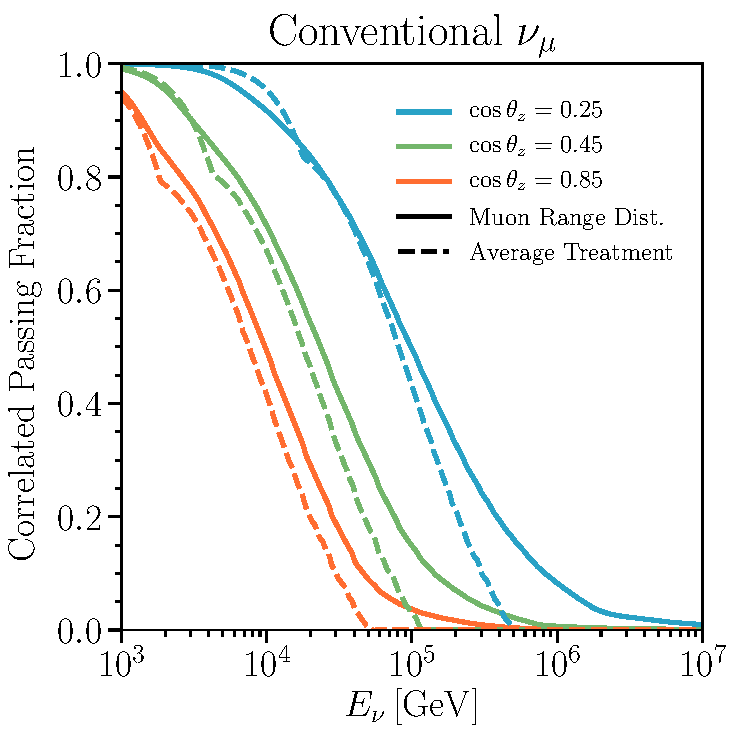
\includegraphics[width=0.45\linewidth]{results/passing_fractions_paper/fig/fig6_numu_conv_corr_only_murange_vs_avg}
	}
	\subfloat{
		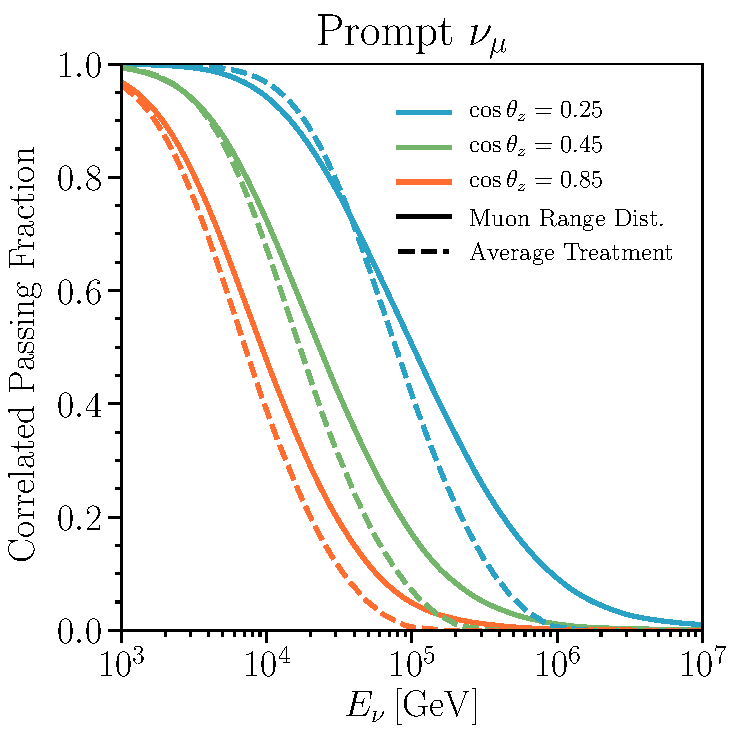
\includegraphics[width=0.45\linewidth]{results/passing_fractions_paper/fig/fig6_numu_prompt_corr_only_murange_vs_avg}
	}
	\caption{\textbf{\textit{Correlated passing fractions: effect of the treatment of muon losses in ice.}} Same as Fig.~\ref{fig:nue_passing-preach-effect} but only for the correlated part of the passing fraction for $\nu_\mu$.}
	\label{fig:nu-mu-correlated-preach-effect}
\end{figure}

In the same way that we compared different muon treatments for the uncorrelated passing fraction, Fig.~\ref{fig:nu-mu-correlated-preach-effect} shows the effect for the correlated passing fraction.
As the correlated case is only concerned with a single muon where energy is correlated with the neutrino, and energy dependent effect emerges.
For lower energies the muon detection probability is underestimated with the median treatment, resulting in a passing fraction that is too high while the converse is true for higher energies.
This effect is less pronounces in the horizontal region, as the energy correlation becomes more washed out with larger overburden.

As an approximation to the passing fraction, the correlated and uncorrelated passing fractions can be multiplied together like in~\cite{Gaisser:2014bja}.
Using the median muon behavior, the $2$-body approximation, and multiplying the two passing fractions we can obtain the same approximation to the passing fraction as in~\cite{Gaisser:2014bja}
\begin{equation}
\label{eq:PGJKvS}
\Prob_{\rm pass}^{\rm GJKvS} (E_\nu, \theta_z) \equiv \Prob_{\rm pass}^{\rm cor, SGRS}(E_\nu, \theta_z) \, \Prob_{\rm pass}^{\rm uncor, GJKvS}(E_\nu, \theta_z) ~,
\end{equation}
which contains the correlated passing fraction derived in~\cite{Schonert:2008is}
\begin{equation}
\label{eq:PcorSGRS}
\Prob_{\rm pass}^{\rm cor, SGRS}(E_\nu, \theta_z) = \frac{1}{\phi_\nu(E_\nu, \theta_z)} \, \sum_A \sum_{p} \int dE_p  \int \frac{dX}{\lambda_p(E_p, X)} \, \frac{dN_{p, \nu}}{dE_\nu}(E_p, E_\nu) \, \phi_{A, p}(E_p, X) \,
\left[1 - \Prob_{\rm det}^{\rm SGRS}\left(E_p-E_\nu , \theta_z\right)\right]~.
\end{equation}

Instead of taking the ``factorized'' approach in Eq.~\ref{eq:PGJKvS}, the correlated and uncorrelated equations can be combined at the level of muon detection, as the veto can be thought of as a logical OR between the detection of an uncorrelated muon and the detection of a sibling muon.
This logical OR can be achieved in the calculation by the multiplication of the non-detection probabilities $\Pzm = \Pzmsib \Pzmproto$.
Similarly weighting the integrand in the neutrino flux calculation by this quantity and maintaining the energy correction described previously, the complete passing fraction is obtained
\begin{align}
\label{eq:GUE}
\Prob_{\rm pass}(E_\nu, \theta_z) = \frac{1}{\phi_\nu(E_\nu, \theta_z)} \, \sum_A \sum_{p} & \int dE_p  \int \frac{dX}{\lambda_p(E_p, X)} \int d\ECR \, \frac{dN_{p, \nu}}{dE_\nu}(E_p, E_\nu) \, \frac{dN_{A, p}}{dE_p}(\ECR, E_p, X) \, \phi_A(\ECR) \nonumber \\
& \times \Pzmsib \left(\theta_z|E_p, E_\nu \right) \, \Pzmproto\left(N_\mu=0;  \bar N_{\mu, A}(\ECR - E_p, \theta_z) \right).
\end{align}
The numerator in the above equation corresponds to the passing flux $\phi_\nu^{\rm pass}(E_\nu, \theta_z)$.
This represents the final equation to be used in the passing fraction calculation as all the relevant effects are accounted for, save for the approximations described earlier.
Eq.~\ref{eq:GUE} naturally applies to muon neutrinos, but also can be directly applied to electron neutrinos for which no sibling muons are present meaning $\Pzmsib \left(\theta_z | E_p, E_\nu \right) = 1$.
Setting the sibling non-detection probability to 1 recovers the result for electron neutrinos in Eq.~(\ref{eq:PuncorGUE}).
Expanding the probabilities in the above equation, the explicit result is
\begin{align}
\label{eq:GUEexplicit}
\Prob_{\rm pass} (E_\nu, \theta_z) = & \frac{1}{\phi_\nu(E_\nu, \theta_z)} \, \sum_A \sum_{p} \int dE_p \int \frac{dX}{\lambda_p(E_p, X)} \int d\ECR \, \frac{dN_{p, \nu}}{dE_\nu}(E_p, E_\nu) \, \frac{dN_{A, p}}{dE_p}(\ECR, E_p, X) \, \phi_A(\ECR) \nonumber \\
& \times \left[ 1 - \int \, d\Emi \, \frac{dN_{p, \mu}}{d\Emi}(E_p, E_\nu, \Emi) \, \int d\Emf \, \Prob_{\rm light}(\Emf)  \, \Prob_{\rm reach}\left(\Emf | \Emi, \theta_z\right) \right] \, e^{-N_{A, \mu}(\ECR - E_p, \theta_z)}  ~,
\end{align}

\begin{figure}
	\centering
	\subfloat{
		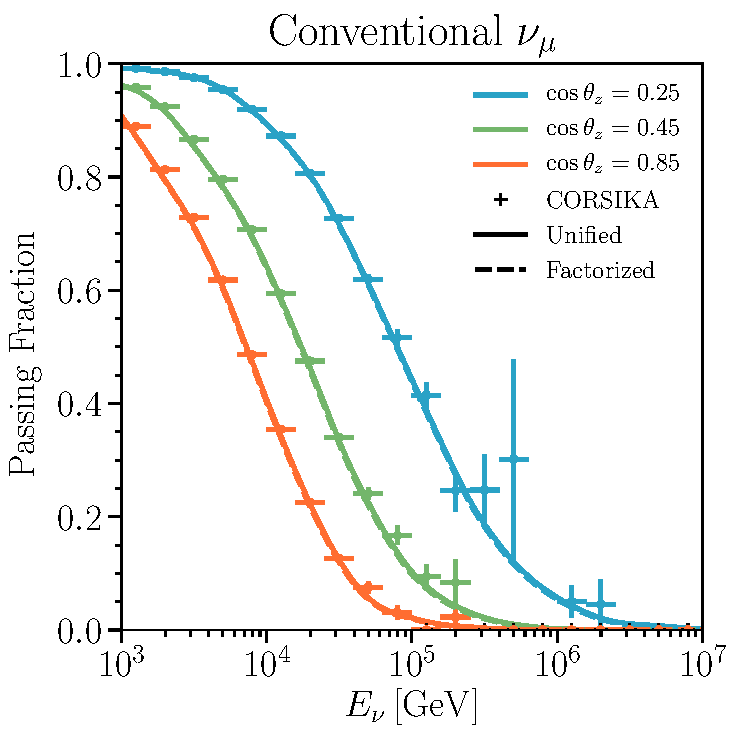
\includegraphics[width=0.45\linewidth]{results/passing_fractions_paper/fig/fig7_b_numu_convetional_unified_versus_factorized_with_corsika_sibyll_23}
	}
	\subfloat{
		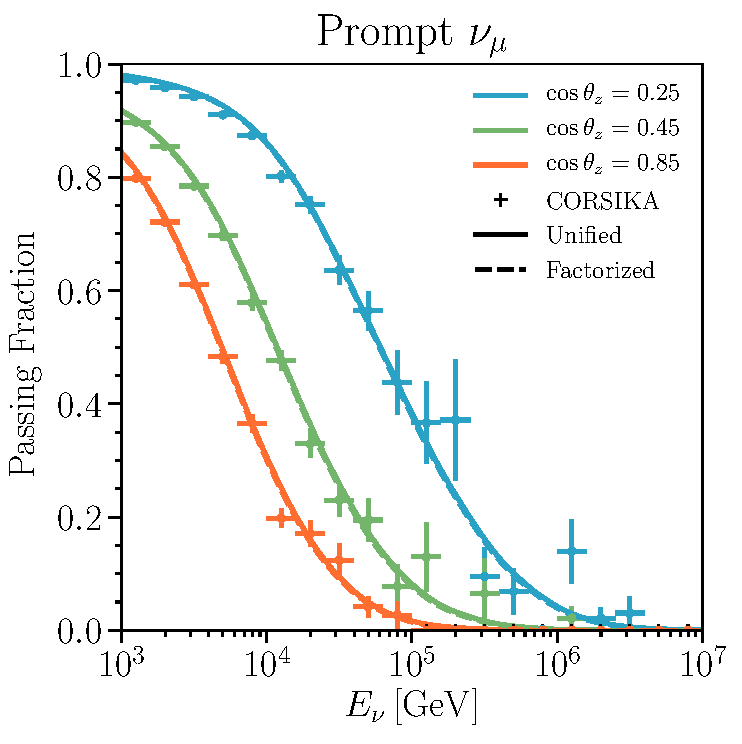
\includegraphics[width=0.45\linewidth]{results/passing_fractions_paper/fig/fig7_a_numu_prompt_unified_versus_factorized_with_corsika_sibyll_23}
	}
	\caption{\textbf{\textit{Passing fractions: differences between the unified and the factorized treatments for $\boldsymbol{\nu_\mu}$.}} Same as Fig.~\ref{fig:nue_passing-double-counting} regarding the approximations on the energy of the shower which gives rise to uncorrelated muons. Comparison of the unified treatment (solid), Eq.~(\ref{eq:GUE}), and the approximate treatment (dashed), Eq.~(\ref{eq:PGJKvS}), which factorizes the correlated and uncorrelated passing fractions. The result is driven by the correlated part.}
	\label{fig:nu-mu-unified-effect}
\end{figure}

The factorized and unified approaches are compared in Fig.~\ref{fig:nu-mu-unified-effect}, where one can see that the differences are negligible compared to the other effects discussed in this section.
The effect of the energy correction $\ECR-E_p$ is smaller for muon neutrinos than in the for electron neutrinos, shown in Fig.~\ref{fig:nue_passing-double-counting}, because for muon neutrinos $\Pzmsib$ is a much more dominant factor than $\Pzmproto$.
Note, for the uncorrelated part of the passing fraction, this subtraction is more important at higher energies, where the correlated contribution is very small.
Thus, the relative effect on the muon neutrino passing fraction is much smaller.
Finally, comparisons of the passing fractions calculated for muon neutrinos and muon antineutrinos are shown in Fig.~\ref{fig:nu-mu-neutrino-vs-antineutrino} and exhibit very good agreement with the Monte Carlo results, as in the case of electron neutrinos (Fig.~\ref{fig:nu-e-neutrino-vs-antineutrino}).

\begin{figure}
	\centering
	\subfloat{
		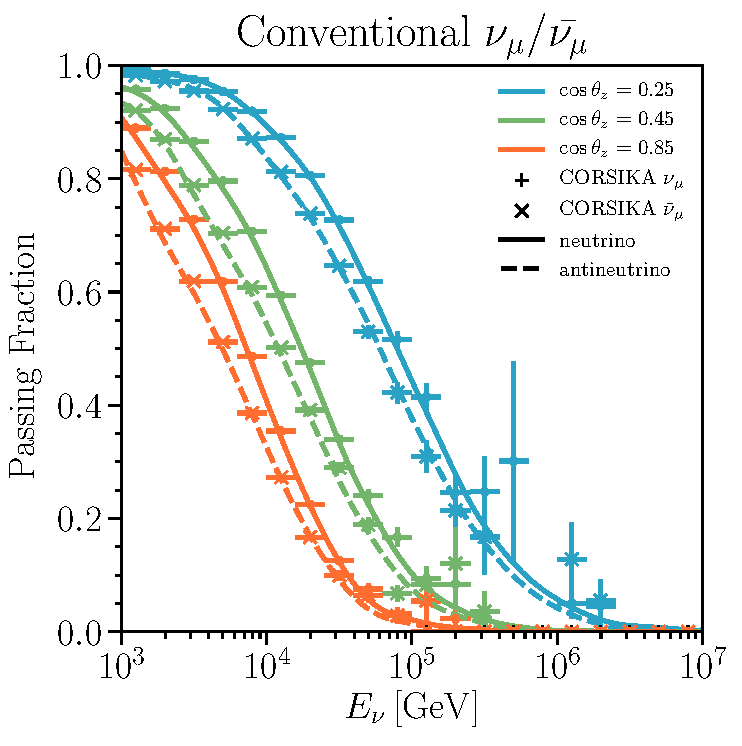
\includegraphics[width=0.45\linewidth]{results/passing_fractions_paper/fig/fig8_b_conventional_numu_versus_numubar_sibyll_23}
	}
	\subfloat{
		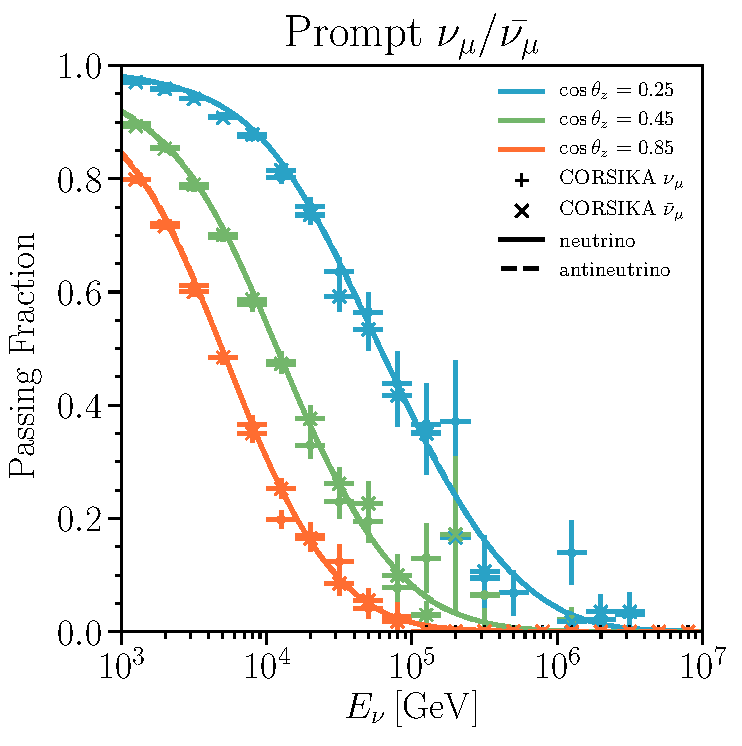
\includegraphics[width=0.45\linewidth]{results/passing_fractions_paper/fig/fig8_a_prompt_numu_versus_numubar_sibyll_23}
	}
	\caption{\textbf{\textit{Passing fractions: neutrinos versus antineutrinos.}} Same as Fig.~\ref{fig:nu-e-neutrino-vs-antineutrino} but for $\nu_\mu$ and $\bar\nu_\mu$. Note that for prompt neutrinos there are not differences between $\nu_\mu$ and $\bar\nu_\mu$.}
	\label{fig:nu-mu-neutrino-vs-antineutrino}
\end{figure}

A comparison of both the neutrino and antineutrino calculations to results from the CORSIKA simulation is shown in Fig.~\ref{fig:nu-mu-neutrino-vs-antineutrino}.
As with the calculation for electron neutrinos, the muon neutrino calculation shows excellent agreement with the air-shower simulations.

\subsubsection{Calculation improvements}

The calculation described in previous sections has many improvements with respect to earlier treatments.
A review of some earlier calculations will help us to examine the differences.

The first proposed calculation of the doing-going atmospheric neutrino suppression due to muons accounted only for sibling muons produced by the same parent meson as the neutrino.
This meant that the original calculation could only be applied to atmospheric muon neutrinos~\cite{Schonert:2008is}.
This original calculation used several analytic approximations, applicable to neutrinos produced in pion and kaon decays under the assumption of a power-;aw cosmic ray primary spectrum.
As described previously, the muon energy loss behavior for this calculation was treated using the median approximation, and the triggering probability modeled asa a Heaviside function.
These choices allowed analytic passing fractions to be derived.

In~\cite{Gaisser:2014bja} the analytic treatment was generalized to include muons from other branches of the shower, not associated with the production of the neutrino.
This generalization allowed the suppression to be computed for atmospheric electron neutrinos.
Analytic approximations were used to describe the average properties of muons from air showers.
In fact, the calculation in~\cite{Gaisser:2014bja} fit a parameterized $\bar N_{A,\mu}(\ECR, \theta_z)$ to the the results of CORSIKA simulation which sed SIBYLL 2.1 for conventional neutrinos and DMPJET-2.5 for prompt neutrinos.
The combination of these correlated and uncorrelated contributions led to Eq.~\ref{eq:PGJKvS}.
For these two calculations, the components were factorized and the $\ECR-E_p$ subtraction was not performed.
This led to an overestimation of the shower energy producing visible muons for the electron neutrino case.

The new approach, explained in the previous sections and developed in~\cite{Arguelles:2018awr} includes a full description of the cosmic ray primary spectrum and composition as well as the hadronic interactions that give rise to the parent particles and eventually muons and neutrinos.
This leads to the more accurate Eq.~\ref{eq:GUE} which is fully consistent between electron and muon neutrinos, although it must be calculated numerically.
Muon energy loss distributions are also fully accounted for in this treatment.
Critically, this approach uses numerical techniques instead of analytic approximations, opening the door for a wide array of modifications to the calculation.
These modifications can include: different detector configurations and responses, cosmic ray spectra, hadronic interaction models, atmospheric density models, and muon energy loss cross sections.
With these modifications the passing fraction calculation can be made consistent with the modern atmospheric neutrino flux calculations of $\MCEq$.

\begin{figure}
	\centering
	\subfloat{
		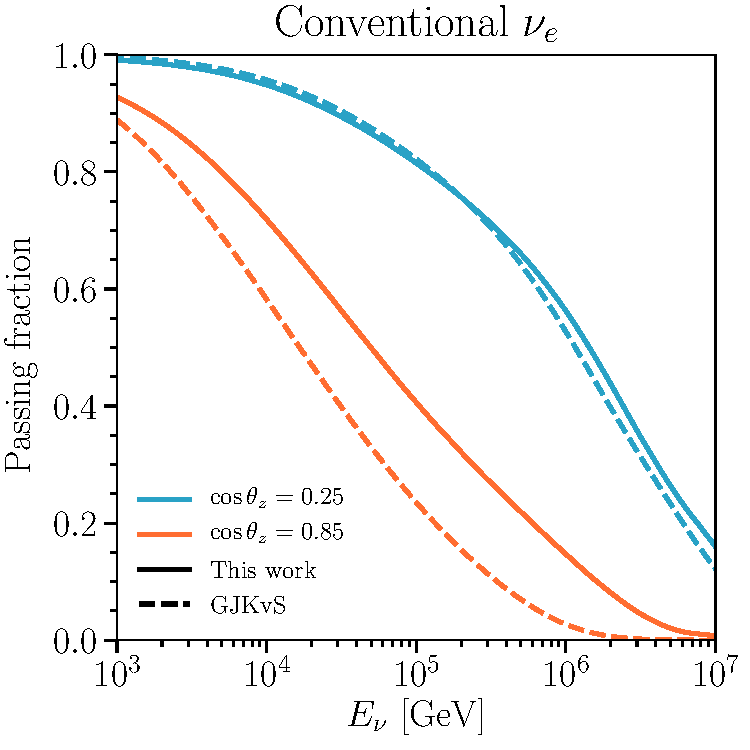
\includegraphics[width=0.45\linewidth]{results/passing_fractions_paper/fig/fig9_extsv_conv_nue}
	}
	\subfloat{
		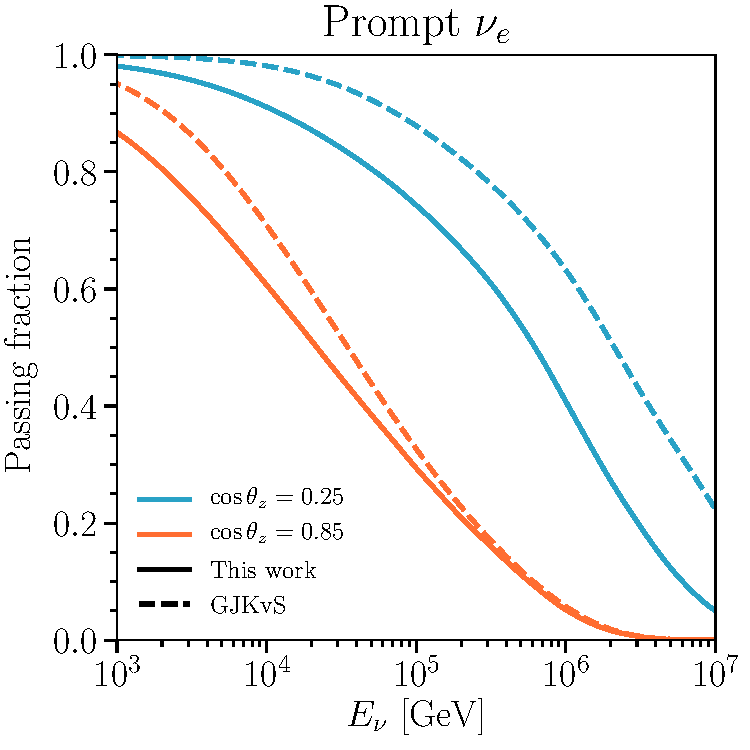
\includegraphics[width=0.45\linewidth]{results/passing_fractions_paper/fig/fig9_extsv_pr_nue}
	} \\[2ex]
	\subfloat{
		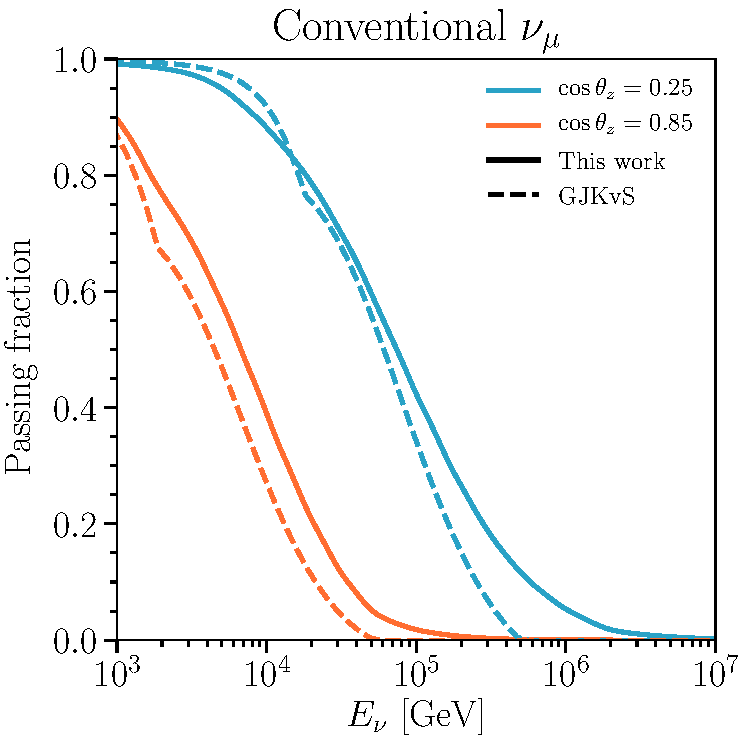
\includegraphics[width=0.45\linewidth]{results/passing_fractions_paper/fig/fig9_extsv_conv_numu}
	}
	\subfloat{
		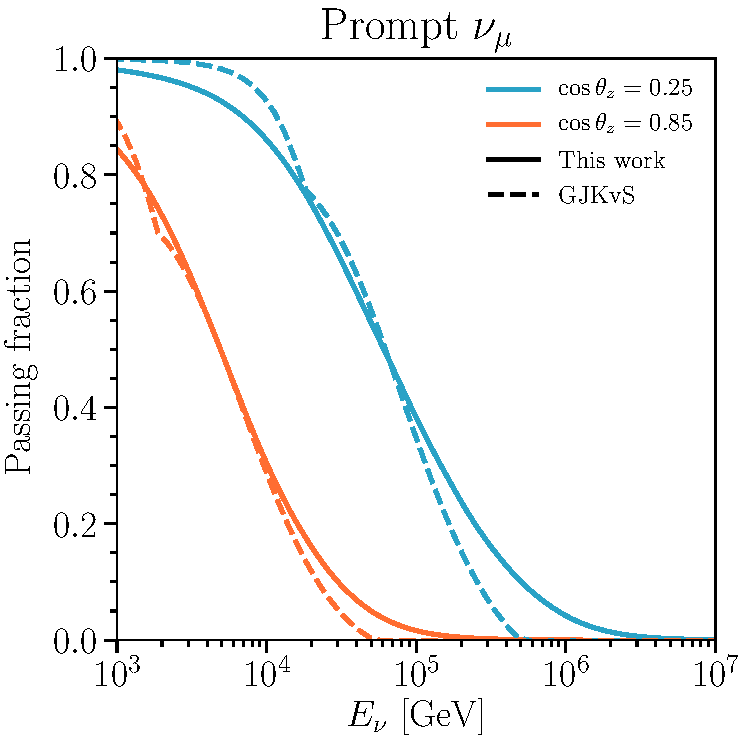
\includegraphics[width=0.45\linewidth]{results/passing_fractions_paper/fig/fig9_extsv_pr_numu}
	}
	\caption{\textbf{\textit{Passing fractions: comparison with previous work}}. Results are shown for two values of $\cos\theta_z =$ (from top to bottom): 0.25 (blue) and 0.85 (orange); with the calculation in this work (solid) and with that in Ref.~\cite{Gaisser:2014bja} (dashed). Our results are obtained with the H3a primary cosmic-ray spectrum~\cite{Gaisser:2011cc}, the SIBYLL~2.3c hadronic-interaction model~\cite{Riehn:2017mfm}, the MSIS-90-E atmosphere-density model at the South Pole on July 1, 1997~\cite{Labitzke:1985, Hedin:1991}, and assuming $d_{\rm det} = 1.95$~km in ice and $\Prob_{\rm light}(\Emf) = \Theta(\Emf - 1\,{\rm TeV})$. They include all of the effects discussed in previous sections, Eq.~(\ref{eq:GUE}). \textit{Top-left panel:} Conventional $\nu_e$ passing fraction. \textit{Top-right panel:} Prompt $\nu_e$ passing fraction. \textit{Bottom-left panel:} Conventional $\nu_\mu$ passing fraction. \textit{Bottom-right panel:} Prompt $\nu_\mu$ passing fraction.}
	\label{fig:nue-passing-comparison-old}
\end{figure}

Fig.~\ref{fig:nue-passing-comparison-old} shows a direct comparison between the new calculation and its predecessor~\cite{Gaisser:2014bja} for $\nu_e$ and $\nu_\mu$ from the conventional and prompt fluxes in two different directions.
In the more vertical direction, $\nu_e$ and $\nu_\mu$ passing fractions for the conventional flux show a large difference, where the newer calculation provides a higher passing fraction.
Two effects are important here, the muon range treatment and the energy of the uncorrelated shower branch.
Near the horizon these effects partially cancel, minimizing the difference between the two calculations, but that is not the case in the vertical direction.
The shoulder present in the older calculation shows the transition between the pion and kaon dominated production of neutrinos, however this is washed out by the more detailed muon range treatment of the new calculation.
The differences in the prompt $\nu_e$ curves are more difficult to interpret.
Comparisons of the muon range treatment and the energy subtraction for prompt $\nu_e$ would lead us to expect some small differences, but not quite of this magnitude.
One additional factor that could explain this, is the use of DPMJET-2.55 in the old calculation for prompt neutrinos; we see that DPMJET-2.55 gives larger passing fractions than SIBYLL 2.3c.
Differences in the prompt $\nu_\mu$ passing fractions are explained by the fact that~\cite{Gaisser:2014bja} applies the conventional $\nu_\mu$ passing fractions to prompt $\nu_\mu$.

\subsubsection{Calculation systematics}
The calculation outlines in these sections relies on a host of external information such as the cosmic ray flux, the physics governing decays and hadronic interactions, calculations of muon energy loss cross sections, and the detector response.
In this section, a few of these potential sources of uncertainty are examined.

\paragraph{Muon Energy Losses}
Muons lose energy in a medium through three processes: ionization losses, $e^+e^-$ pair production, bremsstrahlung, and photo-nuclear interactions.
Below $\sim\SI{1}\TeV$ losses are dominated by ionization.
Whereas, at higher energies the radiative processes dominate.
In order of importance these are pair production, bremsstrahlung, and photo-nuclear interactions.
Above $\sim\SI{10}\PeV$ photo-nuclear interactions are comparable to bremsstrahlung~\cite{Chirkin:2004hz}.
These processes are well understood up to $\sim\SI{10}\TeV$ in muon energy, above which the photo-nuclear interactions dominate the uncertainty in the cross section.

The photo-nuclear cross section used in MMC/PROPOSAL by default uses a data-driven parameterization of the proton structure function in a deep-inelastic scattering (DIS) formalism~\cite{Abramowicz:1991xz, Abramowicz:1997ms}.
This formalism includes contributions from both soft (non-perturbative) and hard (perturbative) physics~\cite{Dutta:2000hh}.
Another approach describes the cross section with a generalized vector dominance model for the soft component~\cite{Bezrukov:1981ci} and a framework of the color dipole moment for the hard component~\cite{Bugaev:2002gy, Bugaev:2003sw}.

Without appropriate measurements and the corresponding data-derived uncertainties the cross section uncertainty can be examined by comparing the two calculation approaches.
At the energies relevant for the passing fraction calculation the default cross sections are slightly lower, resulting in smaller passing fractions as more muons can reach the detector with higher energy.
These differences in the cross section result in a maximum difference of 0.01 for the passing fractions.

\paragraph{Primary Cosmic Ray Spectra}
Previously shown comparisons all assume the Hillas-Gaisser three population model (H3a)~\cite{Gaisser:2011cc}.
This model considers five different nuclei mass groups with three populations.
These cut off at a characteristic rigidity.
Other models for the cosmic ray primary flux have been proposed, and current measurements leave a considerable amount of uncertainty in the energy regime relevant for the passing fractions.

A second model, GST-4gen~\cite{Gaisser:2013bla}, has a lower cutoff for the first two populations which also have correspondingly harder spectra.
While the third population is iron-only above the spectrum ankle.
A fourth proton-only component is included to obtain better agreement with shower depth data around $\SI{1}\EeV$.
However, this proton-iron composition is somewhat in tension with data from Auger~\cite{Abraham:2010yv, Aab:2014aea}.

A third model, ZS~\cite{Zatsepin:2006ci}, has three components derived from specific astrophysical sources.
The lowest energy population comes from the expanding shells of supernovae remnants.
The middle energy component comes from isolated supernovae and their interaction with the interstellar medium.
Finally, the high energy component comes from massive star supernovae explosions and their interaction with their own stellar wind.
This last process produces a very heavy composition.

\begin{figure}[h!]
	\centering
	\subfloat{
		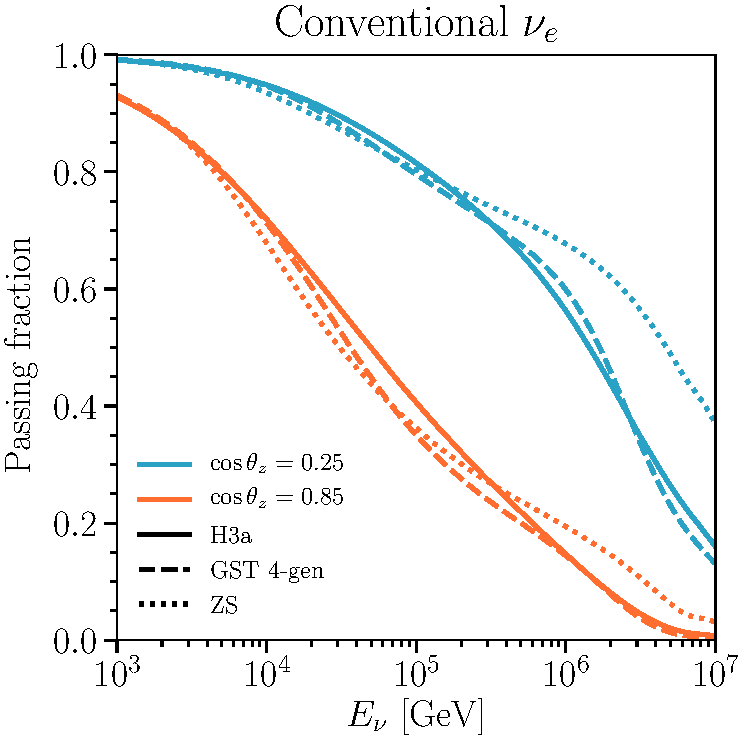
\includegraphics[width=0.45\linewidth]{results/passing_fractions_paper/fig/fig10_pmodels_conv_nue}
	}
	\subfloat{
		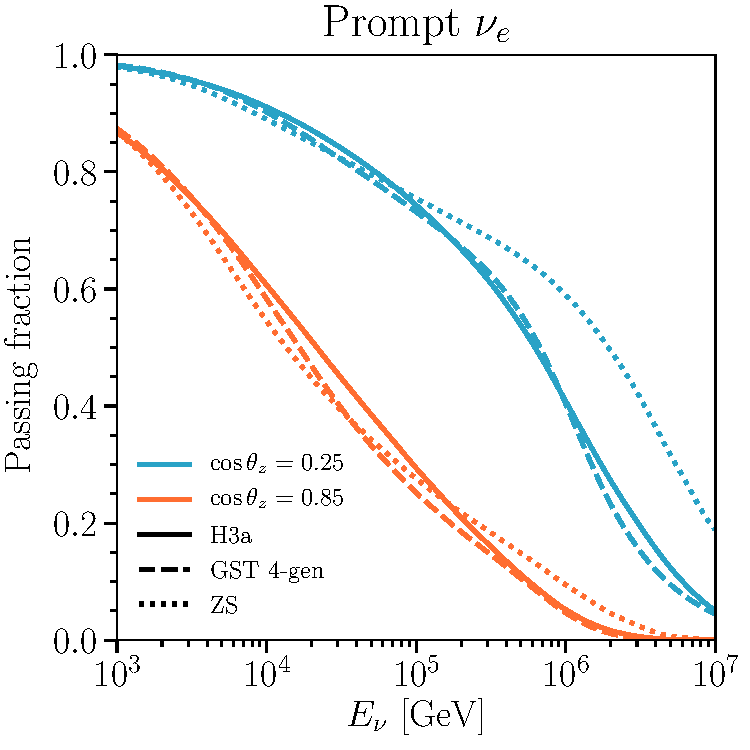
\includegraphics[width=0.45\linewidth]{results/passing_fractions_paper/fig/fig10_pmodels_pr_nue}
	}\\[2ex]
	\subfloat{
		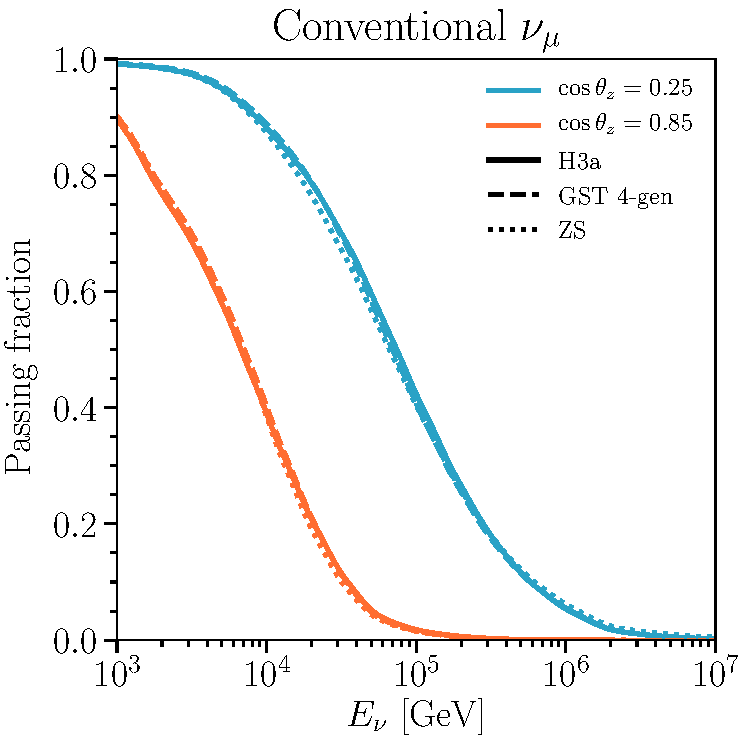
\includegraphics[width=0.45\linewidth]{results/passing_fractions_paper/fig/fig10_pmodels_conv_numu}
	}
	\subfloat{
		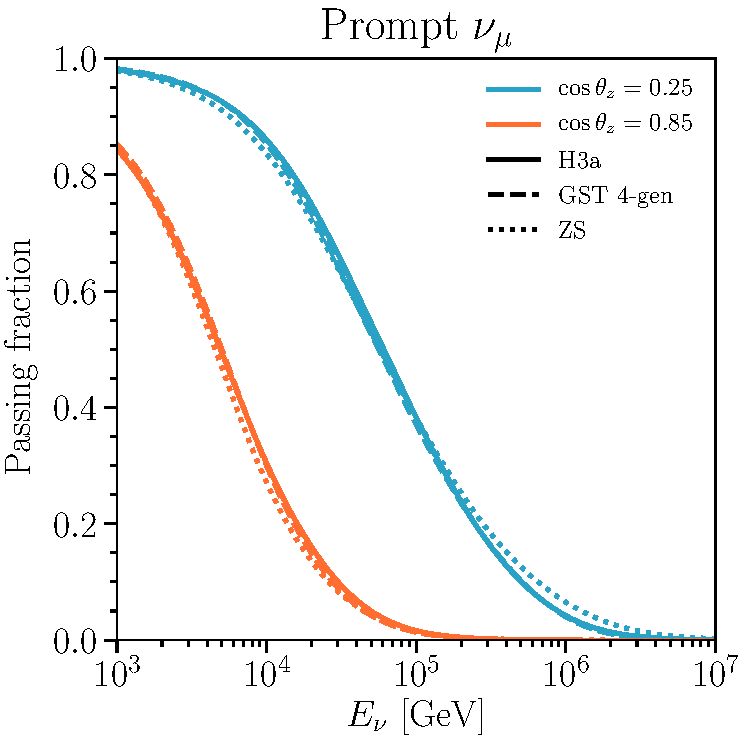
\includegraphics[width=0.45\linewidth]{results/passing_fractions_paper/fig/fig10_pmodels_pr_numu}
	}
	\caption{\textbf{\textit{Passing fractions: effect of primary cosmic-ray spectrum}}. Results are shown for two values of $\cos\theta_z$ (from top to bottom): 0.25 (blue) and 0.85 (orange); for four CR models: Hillas-Gaisser H3a~\cite{Gaisser:2011cc} (solid), Gaisser, Stanev and Tilav (GST 4-gen)~\cite{Gaisser:2013bla} (dashed) and Zatsepin-Solkolskaya (ZS)~\cite{Zatsepin:2006ci} (dotted).
		\textit{Top-left panel:} Conventional $\nu_e$ passing fraction. \textit{Top-right panel:} Prompt $\nu_e$ passing fraction. \textit{Bottom-left panel:} Conventional $\nu_\mu$ passing fraction. \textit{Bottom-right panel:} Prompt $\nu_\mu$ passing fraction.}
	\label{fig:nue-cr-model-effect} \vspace{1.5cm}
\end{figure}

These three models are compared by their effect on the passing fraction calculations in Fig.~\ref{fig:nue-cr-model-effect}.
The largest differences are for the $\nu_e$ passing fractions, which differ between models by less than 0.05 except when comparing the ZS model above $\SI{e6}\GeV$.
This can be understood as a consequence of the ZS model being designed only to describe the cosmic ray flux up to $\SI{e8}\GeV$, meaning the ZS neutrinos flux predictions may not be accurate above $\SI{e6}\GeV$.
The muon neutrinos passing fractions have much smaller variations between models.
This is likely a result fo the sister muons dominating the passing fraction calculation, meaning that the population of showers from which the neutrino may have originated is a subdominant effect.
The level of variation seen between these models represents a non-negligible uncertainty in the passing fractions for electron neutrinos, but is small for muon neutrinos.
However, this level of uncertainty alone is likely to be smaller than the statistical uncertainties currently present for the HESE sample.

Here a bracketing approach was used to examine the uncertainties, and models chosen to express a range of possibilities currently allowed by experimental measurements.
But this is not a full accounting of the cosmic ray flux uncertainties.
The measurement uncertainties can be accounted for in a more satisfactory manner with a non-parametric fit with sufficient degrees of freedom to the available cosmic-ray data.
For any point in the parameter space of this fit both the neutrino flux and passing fraction can be computed to provide an expectation for the ``apparent'' neutrino flux.
By directly using estimates from this fit and allowing the cosmic ray model to vary in a fit of neutrino data the uncertainties can be treated appropriately.
This method has some computational challenges as it is not feasible to run the necessary MCEq calculations each time a different point in the parameter space is tested.
However, there are some optimizations that can be found by carefully examining the basis functions used for the different cosmic ray populations and pre-computing or caching information where applicable.
Such a treatment is not used for the HESE 7.5 year analysis, but may prove to be useful for future analyses that combine multiple samples with more than 10 years of data.

\paragraph{Hadronic Interaction Models}
The muons and neutrinos relevant for this calculation are produced in high energy extensive air showers, the development of which is governed by hadronic interaction physics.
However, these showers and hadronic interactions occur at energies that are orders of magnitude beyond what is accessible to collider experiments where these interactions can be measured.
Thus, our predictions for how these showers develop depends heavily on hadronic models that may are tuned to collider data but are extrapolations at the energies we are concerned with.

\begin{figure}[h!]
	\centering
	\subfloat{
		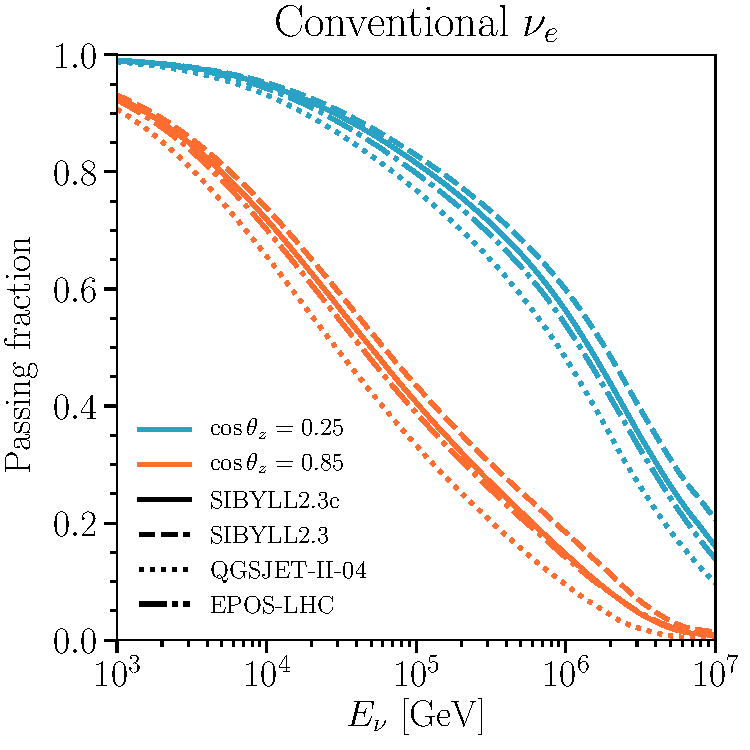
\includegraphics[width=0.45\linewidth]{results/passing_fractions_paper/fig/fig11_hadrs_conv_nue}
	}
	\subfloat{
		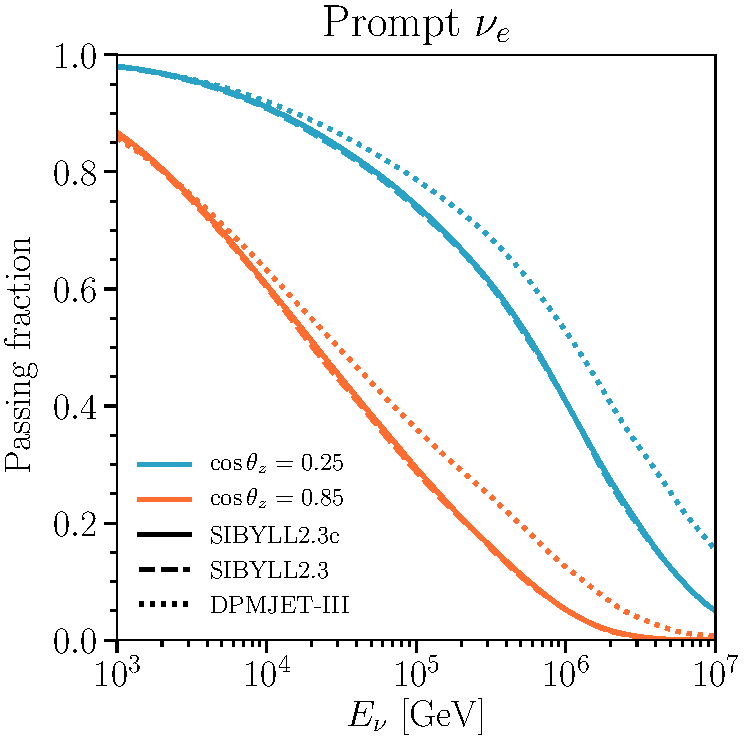
\includegraphics[width=0.45\linewidth]{results/passing_fractions_paper/fig/fig11_hadrs_pr_nue}
	}\\[2ex]
	\subfloat{
		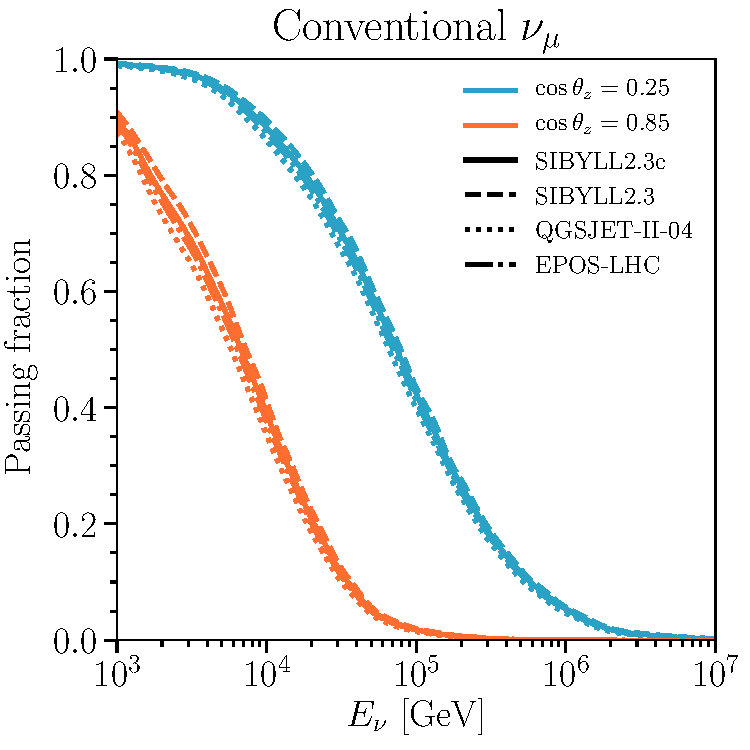
\includegraphics[width=0.45\linewidth]{results/passing_fractions_paper/fig/fig11_hadrs_conv_numu}
	}
	\subfloat{
		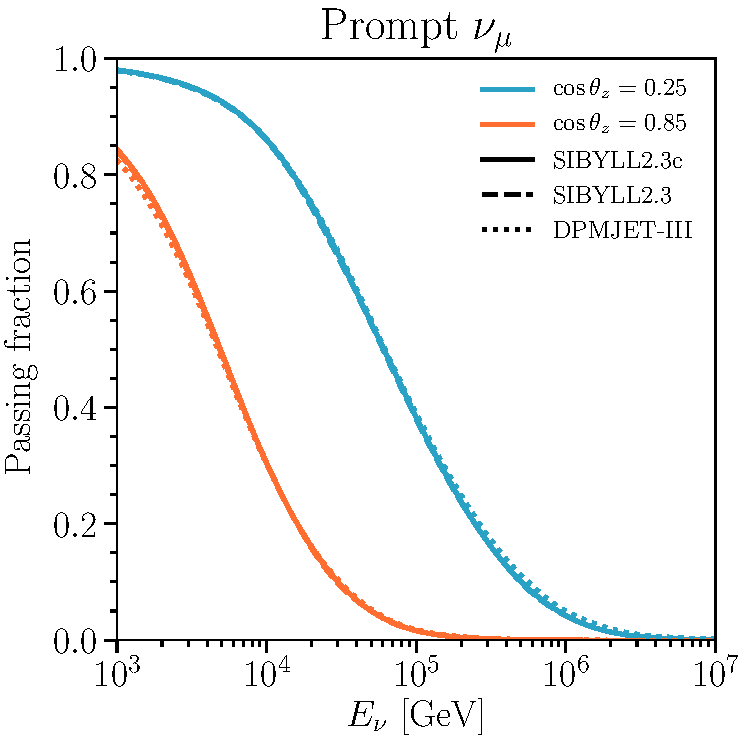
\includegraphics[width=0.45\linewidth]{results/passing_fractions_paper/fig/fig11_hadrs_pr_numu}
	}
	\caption{\textbf{\textit{Passing fractions: effect of hadronic-interaction model}}. Results are shown for two values of $\cos\theta_z$ (from top to bottom): 0.25 (blue) and 0.85 (orange); for different hadronic-interaction models: SIBYLL~2.3c~\cite{Riehn:2017mfm} (solid), SIBYLL~2.3~\cite{Engel:2015dxa, Riehn:2015oba} (dashed), QGSJET-II-04~\cite{Ostapchenko:2010vb} (dotted in left panel), EPOS-LHC~\cite{Pierog:2013ria} (dash-dotted in left panel) and DPMJET-III\cite{Roesler:2000he} (dotted in right panel).
		\textit{Top-left panel:} Conventional $\nu_e$ passing fraction. \textit{Top-right panel:} Prompt $\nu_e$ passing fraction. \textit{Bottom-left panel:} Conventional $\nu_\mu$ passing fraction. \textit{Bottom-right panel:} Prompt $\nu_\mu$ passing fraction.} \vspace{1cm}
	\label{fig:nue-hadronic-model-effect}
\end{figure}

Figure~\ref{fig:nue-hadronic-model-effect} shows a comparison of the passing fractions computed assuming four different hadronic interaction models.
A detailed discussion of the differences between these models can be found in Section IV.C of~\cite{Arguelles:2018awr}.
For electron neutrinos there are non-negligible differences in the passing fractions, but the variation is again small for muon neutrinos.

\paragraph{Depth and Surrounding Medium}
In these sections a depth of $\SI{1.95}\km$ has been assumed to model the veto effects at the center of the IceCube detector.
However, IceCube and other neutrino detectors are large enough that the change in depth from top to bottomo significantly changes the overburden for a neutrino of a given zenith angle.
Increases in the overburden significantly reduce the power of the veto, as muons that reach the detector are fewer and less energetic.
As a benchmark, we can examine the passing fractions assuming a depth of $\SI{3.5}\km$, corresponding to the depth of KM3NeT-Italy, and also compare differences between ice and water.

\begin{figure}[h!]
	\centering
	\subfloat{
		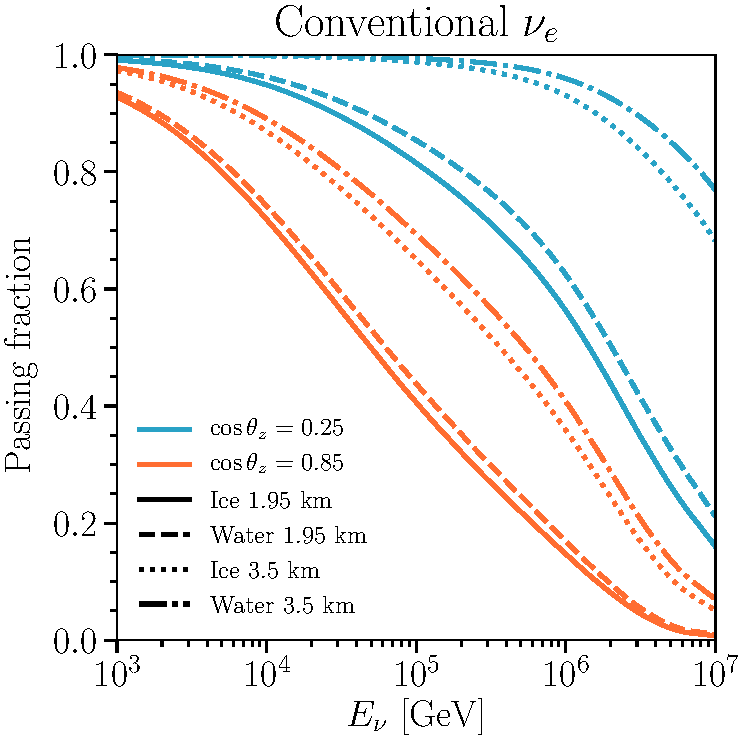
\includegraphics[width=0.45\linewidth]{results/passing_fractions_paper/fig/fig13_medium_conv_nue}
	}
	\subfloat{
		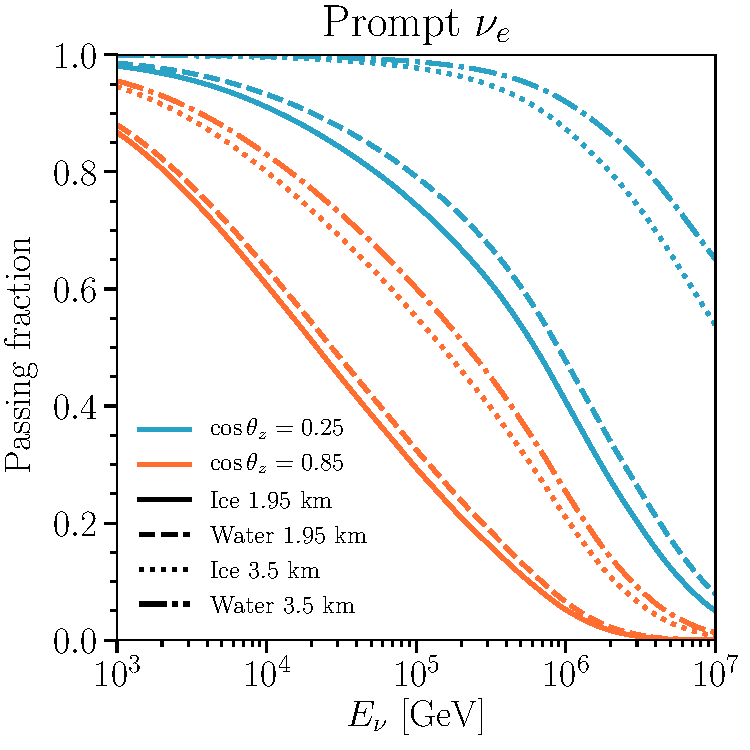
\includegraphics[width=0.45\linewidth]{results/passing_fractions_paper/fig/fig13_medium_pr_nue}
	}\\[2ex]
	\subfloat{
		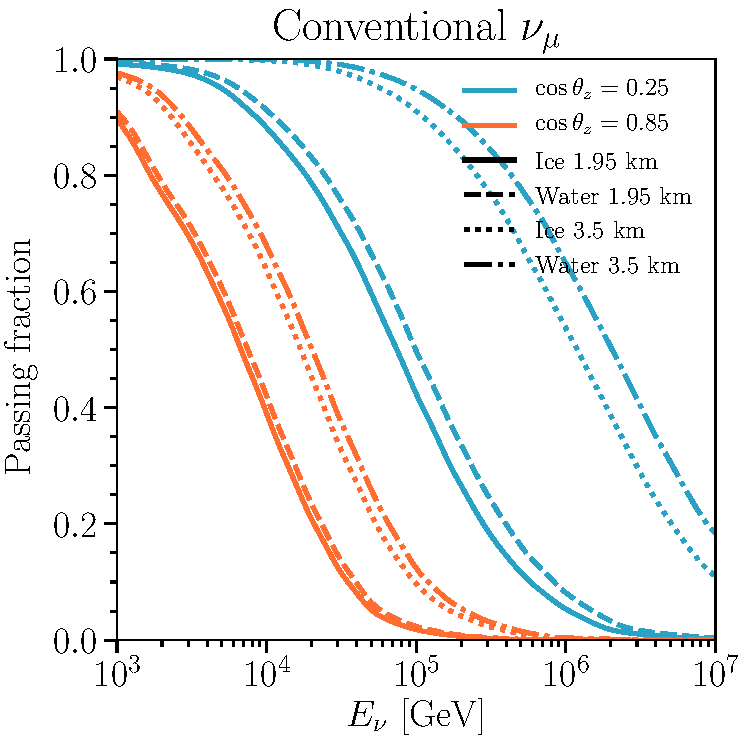
\includegraphics[width=0.45\linewidth]{results/passing_fractions_paper/fig/fig13_medium_conv_numu}
	}
	\subfloat{
		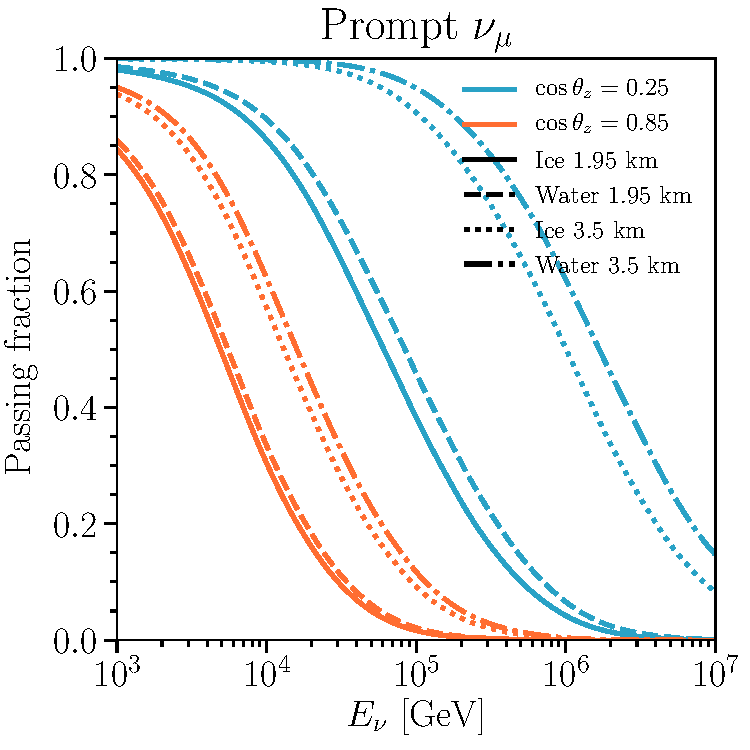
\includegraphics[width=0.45\linewidth]{results/passing_fractions_paper/fig/fig13_medium_pr_numu}
	}
	\caption{\textbf{\textit{Passing fractions: effect of depth/medium}}. Results are shown for two values of $\cos\theta_z$ (from top to bottom): 0.25 (blue) and 0.85 (orange); for two depths: $d_{\rm det} = 1.95$~km (solid and dashed) and $d_{\rm det} = 3.5$~km (dotted and dash-dotted); and for two different media: ice (solid and dotted) and water (dashed and dot-dashed). \textit{Top-left panel:} Conventional $\nu_e$ passing fraction. \textit{Top-right panel:} Prompt $\nu_e$ passing fraction. \textit{Bottom-left panel:} Conventional $\nu_\mu$ passing fraction. \textit{Bottom-right panel:} Prompt $\nu_\mu$ passing fraction.} \vspace{1.5cm}
	\label{fig:medium-effect}
\end{figure}

Figure~\ref{fig:medium-effect} shows these comparisons.
It is notable that the differences between water and ice are non-negligible but much less dramatic than the effect of depth.
As expected, the effect of the surrounding medium is also more pronounced near the horizon where the change in effective overburden is larger.
The increased depth results in a significantly larger passing fraction, greatly reducing the power of veto techniques.
It is therefore important to model the depth of events to accurately determine their passing probability.
Depth is also an important consideration when evaluating the sensitivity of different neutrino detectors to the astrophysical flux.

\paragraph{Detector Response}
The probability for a muon to trigger the veto, $\Prob_{\rm light}$, encapsulates the detector response that is relevant for the passing fraction calculation.
So far in this discussion all the passing fractions have been computed with a $\SI{1}\TeV$ threshold Heaviside $\Prob_{\rm light}$.
While the Heaviside parameterization is simple, the real detector response is certainly more complex.
The particular form of $\Prob_{\rm light}$ will depend on the particulars of the implemented veto.
To get a feel for these differences and the uncertainty that detector response modeling could introduce we look at a few different $\Prob_{\rm light}$ functions.

\begin{figure}[h!]
	\centering
	\subfloat{
		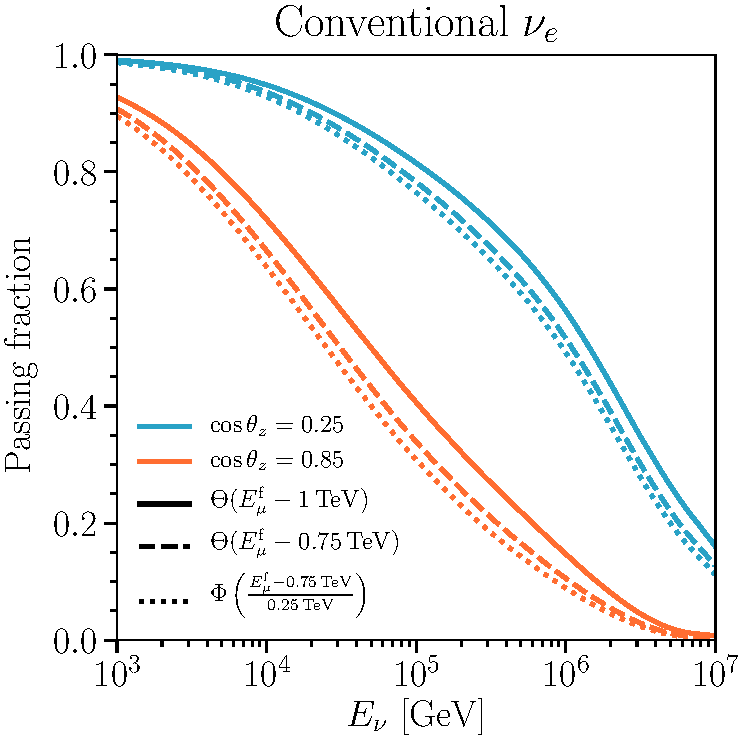
\includegraphics[width=0.45\linewidth]{results/passing_fractions_paper/fig/fig14_pls_conv_nue}
	}
	\subfloat{
		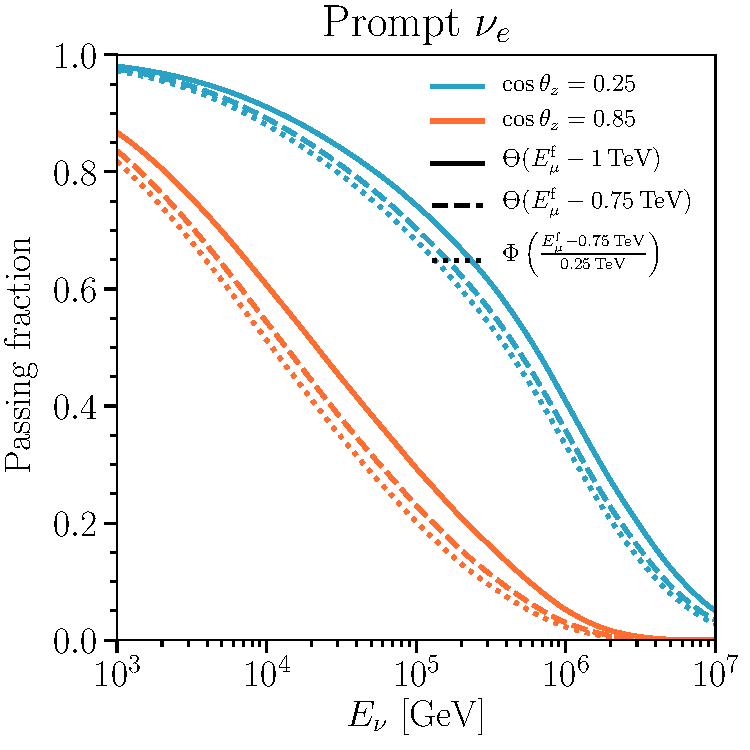
\includegraphics[width=0.45\linewidth]{results/passing_fractions_paper/fig/fig14_pls_pr_nue}
	}\\[2ex]
	\subfloat{
		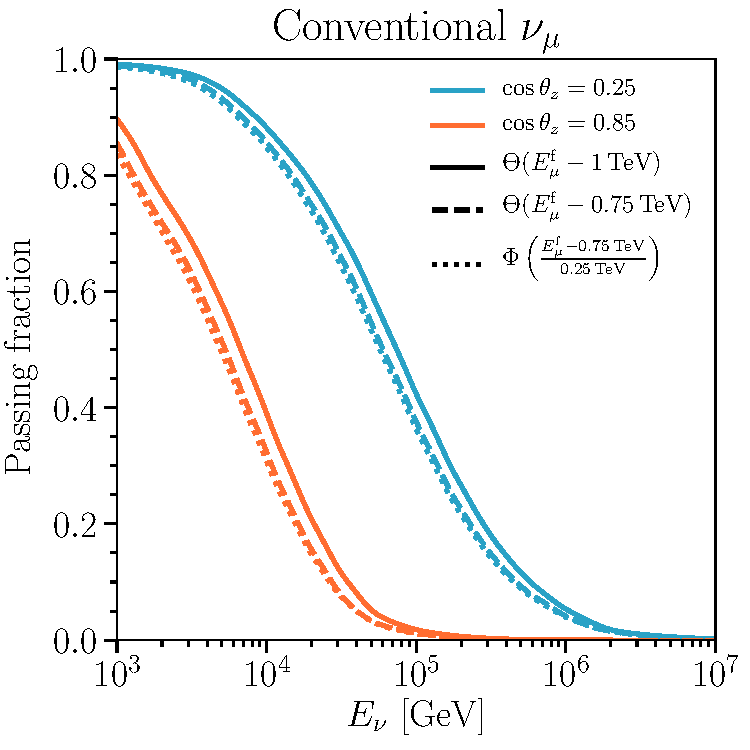
\includegraphics[width=0.45\linewidth]{results/passing_fractions_paper/fig/fig14_pls_conv_numu}
	}
	\subfloat{
		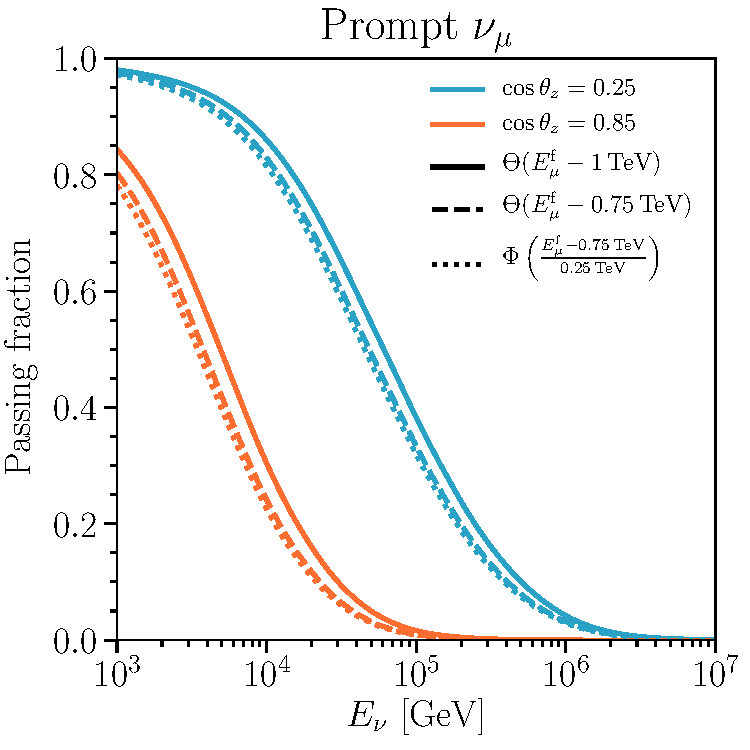
\includegraphics[width=0.45\linewidth]{results/passing_fractions_paper/fig/fig14_pls_pr_numu}
	}
	\caption{\textbf{\textit{Passing fractions: effect of $\boldsymbol{\Prob_{\rm light}}$}}. Results are shown for two values of $\cos\theta_z$ (from top to bottom): 0.25 (blue) and 0.85 (orange); for three different $\Prob_{\rm light}(\Emf)$: a Heaviside with a muon threshold at 1~TeV, $\Theta\left(\Emf - 1 \, {\rm TeV}\right)$ (solid), a Heaviside with a muon threshold at 0.75~TeV, $\Theta\left(\Emf - 0.75 \, {\rm TeV}\right)$ (dashed) and a sigmoid $\Phi\left(\left(\Emf - 0.75 \, {\rm TeV}\right)/0.25 \, {\rm TeV}\right)$ (dotted). \textit{Top-left panel:} Conventional $\nu_e$ passing fraction. \textit{Top-right panel:} Prompt $\nu_e$ passing fraction. \textit{Bottom-left panel:} Conventional $\nu_\mu$ passing fraction. \textit{Bottom-right panel:} Prompt $\nu_\mu$ passing fraction.} \vspace{1.5cm}
	\label{fig:nue-plight-effect}
\end{figure}

With straightforward veto implementations a smooth, monotonic, threshold-like behavior is expected.
This can be understood as a consequence of three factors: cuts on observable parameters, fluctuations in observed light, and the positive correlation between muon energy and light emission.
The cuts on observable parameters introduce the threshold behavior, choosing to accept and reject events that fall into different regions of the observable parameter space.
However, this hard threshold is smoothed out by fluctuations in the observable parameters.
Stochastic energy losses of the muons mean that the emitted light near the veto can vary wildly for identical muons; further variation is caused by photon scattering and the quantum efficiency of the detector PMTs.
The Heaviside function models this threshold behavior but transitions too sharply represent a realistic detector response.
An alternative is to use a sigmoid to model the smooth transition, in this case a logistic function is a reasonable choice.
Figure~\ref{fig:nue-plight-effect} shows the passing fractions for three variations of the $\Prob_{\rm light}$ function, a Heaviside with $\SI{1}\TeV$ threshold, a Heaviside with $\SI{0.25}\TeV$ threshold, and finally a logistic function with a $\SI{0.25}\TeV$ threshold and $1/\SI{0.25}\TeV$ growth parameter.
A reduction in the Heaviside function threshold produces a reduction of the passing fraction as expected.
The change from Heaviside to sigmoid produces a smaller reduction, although this comparison of the effect's magnitude is arbitrary.
Although the change to muon neutrino passing fractions is smaller than that for electron neutrinos, this is the largest change in the muon neutrino passing fraction for a fixed detector geometry.
We should stress the importance of correctly modeling the detector response to muons as it will significantly affect the passing fractions for both flavors.

\subsubsection{HESE passing fractions\label{sec:hese_passingfractions}}
In this approach the neutrino properties are known from simulation, and it is sought to average over all the potential properties of the cosmic ray air showers from which the neutrino could have been produced in.
Ideally this average over air shower properties should be computed for each neutrino position, direction, and energy because the detector response can vary with all six of these parameters.
However, not all of these properties are used directly in the analysis nor does the detector response depend equally on all of these parameters.
For this reason when performing the calculation of the efficiency, only the neutrino energy, zenith angle, and depth upon intersection with the detector are considered.
Other properties of the neutrino are averaged over.
Additionally, in the characterization of the detector response to muons, only dependence on the muon energy and depth are considered.
Thus, the computed passing fraction depends on the neutrino energy, the zenith angle, and the incident depth in the detector.
However, the detector response and neutrino properties can be factorized so that the problem may be discussed more generally.
In previous analyses, the passing fractions were calculated using an extension of the method described in~\cite{Schonert:2008is} and bounded at $\SI{10}\percent$; details of the method are provided in~\cite{Aartsen:2013jdh}.
Cosmic ray simulations remain a computationally prohibitive way of accounting for the effects of accompanying muons, so we still rely on calculations of the average passing rate.
In this analysis, we use the new calculation described above and in~\cite{Arguelles:2018awr} that allows for different cosmic-ray and hadronic models to be used; more importantly for this analysis any parameterization of the detector veto response to muons can be used in the calculation, as opposed to just an energy threshold.
This capability allows us to more accurately model the detector response to atmospheric neutrinos.
In \reffig{fig:P_light} we show the probability that a muon will pass the veto as a function of the true muon incident energy for different detector depths.

% Plot of p_light
\begin{figure}
	\centering
	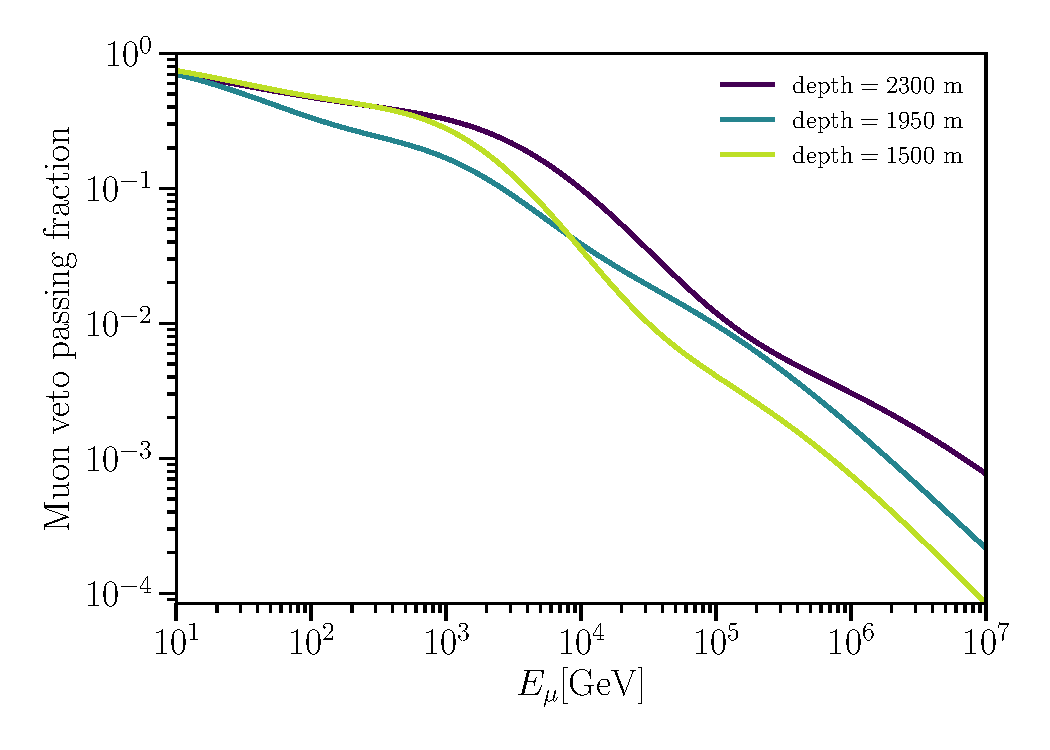
\includegraphics[width=\linewidth]{results/HESE_Final_Paper/figures/plight}
	\internallinenumbers
	\caption{\textbf{\textit{Muon veto passing fraction.}} Each line shows the fraction of muons of a given energy at the detector edge, $E_\mu$, that pass without triggering the veto when entering the detector at a particular depth.
		Three depths are shown: 1500, 1950, and 2300 meters from the surface; with lines of darkening color as the depth increases.
		The veto efficiency increases with the muon energy.
		Differences at various depths are due to the changing ice properties, and varying acceptance as a function of depth due to the asymmetric structure of the veto region.
		At all depths a sigmoid function is fit to the results of muon simulation.
		Above $\sim\SI{100}\TeV$ the passing fraction is extrapolated.}\label{fig:P_light}
\end{figure}

Using the muon passing fractions in \reffig{fig:P_light} as input and the \nuveto{} code provided in~\cite{Arguelles:2018awr} the atmospheric passing fraction is calculated for each component and flavor using the Hillas-Gaisser H3a~\cite{Gaisser:2013bla,Gaisser:2011cc,Hillas:2006ms} model for the incident cosmic-ray spectra and SIBYLL2.3c~\cite{Riehn:2017mfm} for the hadronic interactions in the air shower.
Switching to passing fractions derived from alternative cosmic-ray and hadronic interaction models has sub-leading effects in determination of the astrophysical flux~\cite{Arguelles:2018awr}.
Effects of these systematics were studied by repeating the analysis for different passing fractions that arise from a given combination of cosmic-ray spectrum and hadronic model for a variety of spectra and models that are available in the literature.
We found that the inclusion of these effects in addition to other discrete ice choices mentioned later in \refsec{sec:detector_systematics} increases the reported uncertainty of the astrophysical parameters by at most $\SI{20}\percent$ with respect to errors computed without these effects.
For this reason, these effects are not included in the analysis and are not reflected in the reported errors of any model parameters.
In \reffig{fig:passingfraction} we show the passing fractions for the conventional and prompt neutrino components.
In these figures the left, center, and right panels correspond to $\cos\theta_z$ values of 0.1, 0.3, and 0.9 respectively; the solid lines correspond to muon neutrinos and the dashed lines to electron neutrinos.
From the progression of the panels from left to right, one can see the passing fractions become smaller as one approaches vertical directions.
Vertical muons have the highest probability of reaching the detector, as the overburden they pass through is the smallest.
Though not shown in this figure, the conventional passing fractions differ from neutrinos to anti-neutrinos, see~\cite{Arguelles:2018awr} for details; the appropriate passing fractions are used in this analysis.
\reffigs{fig:conventional_distribution}{fig:prompt_distribution} show the distributions of conventional and prompt neutrinos respectively after this correction is applied.
This reduction in atmospheric background accounts for much of the sensitivity of this analysis to the astrophysical neutrino flux, as the observed down-going atmospheric fluxes in IceCube would otherwise be comparable in magnitude and remain similar in their angular distribution.
This is best seen when comparing the atmospheric fluxes before and after the veto to the measured astrophysical flux as shown in \reffig{fig:neutrino_spectrum}.

% Plot of the passing fraction for different heights (one line per height) (one panel for each costh [3 values])
\begin{figure*}
	\centering
	\subfloat{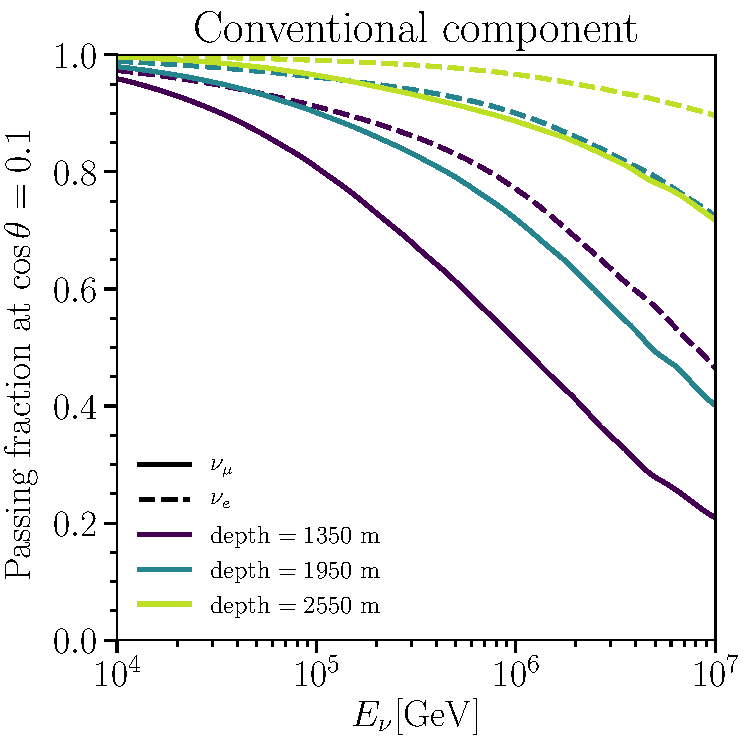
\includegraphics[width=0.3\linewidth]{results/HESE_Final_Paper/figures/conv_0_1_passing_fraction}}
	\subfloat{\includegraphics[width=0.3\linewidth]{results/HESE_Final_Paper/figures/conv_0_3_passing_fraction}}
	\subfloat{\includegraphics[width=0.3\linewidth]{results/HESE_Final_Paper/figures/conv_0_9_passing_fraction}} \\
	\subfloat{\includegraphics[width=0.3\linewidth]{results/HESE_Final_Paper/figures/prompt_0_1_passing_fraction}}
	\subfloat{\includegraphics[width=0.3\linewidth]{results/HESE_Final_Paper/figures/prompt_0_3_passing_fraction}}
	\subfloat{\includegraphics[width=0.3\linewidth]{results/HESE_Final_Paper/figures/prompt_0_9_passing_fraction}}
	\internallinenumbers
	\caption{\textbf{\textit{Conventional and prompt atmospheric component passing fraction.}}
		The top row of plots shows the atmospheric neutrino passing fraction as a function of the neutrino energy for a flux of neutrinos originating from pions and kaons, assuming the Hillas-Gaisser H3a~\cite{Gaisser:2013bla,Gaisser:2011cc,Hillas:2006ms} cosmic-ray model and SIBYLL 2.3c~\cite{Riehn:2017mfm} hadronic interaction model.
		While the bottom row of plots shows the atmospheric neutrino passing fraction for a flux of neutrinos originating from charmed hadrons under the same assumptions.
		Solid lines correspond to muon neutrinos and dashed lines to electron neutrinos.
		The different colors, from darkest to lightest, are for three different detector depths: 1350, 1950, and 2550 meters below the surface.
		The left, center, and right panel correspond to cosine of the zenith angles 0.1, 0.3, and 0.9 respectively (or zenith angles of $\SI{84.3}\degree$, $\SI{72.5}\degree$, and $\SI{25.8}\degree$).}\label{fig:passingfraction}
\end{figure*}

\begin{figure}
	\centering
	\includegraphics[width=\linewidth]{results/HESE_Final_Paper/figures/diffuse_hist_all_conv}
	\internallinenumbers
	\caption{\textbf{\textit{Expected distribution of atmospheric neutrinos produced by pions and kaons in the sample.}} Distribution of neutrinos that pass the veto as a function of the deposited energy and the cosine of the zenith angle assuming nominal values for the nuisance parameters.
		The dashed line at $\SI{60}\TeV$ marks the low energy cut of the analysis.
		Suppression in the down-going region is due to the veto, while suppression in the up-going region is due to absorption of neutrinos in the Earth.}\label{fig:conventional_distribution}
\end{figure}

\begin{figure}
	\centering
	\includegraphics[width=0.8\linewidth]{results/HESE_Final_Paper/figures/diffuse_hist_all_prompt}
	\internallinenumbers
	\caption{\textbf{\textit{Expected distribution of atmospheric neutrinos produced by charmed hadrons in the sample.}} Distribution of neutrinos that pass the veto as a function of the deposited energy and the cosine of the zenith angle assuming nominal nuisance parameters and the BERSS flux calculation for neutrinos from  charmed hadrons~\cite{Bhattacharya:2015jpa}.
		The dashed line at $\SI{60}\TeV$ marks the low energy cut of the analysis.
		Suppression in the down-going region is due to the veto, while suppression in the up-going region is due to absorption of neutrinos in the Earth.}\label{fig:prompt_distribution}
\end{figure}

\begin{figure}
	\centering
	\includegraphics[width=0.8\linewidth]{figures/diffuse_hist_all_astro_fit}
	\internallinenumbers
	\caption{\textbf{\textit{Expected distribution of astrophysical neutrinos from the best-fit spectrum.}} Distribution of neutrinos that pass the veto as a function of the deposited energy and the cosine of the zenith angle assuming the best-fit parameters of an astrophysical power-law spectrum.
	The dashed line at $\SI{60}\TeV$ marks the low energy cut of the analysis.
	Suppression in the up-going region is due to absorption of neutrinos in the Earth, while there is no suppression in the down-going region in the absence of accompanying muons.}\label{fig:astro_distribution}
\end{figure}

\begin{figure}
	\centering
	\includegraphics[width=0.8\linewidth]{results/HESE_Final_Paper/figures/neutrino_spectrum}
	\internallinenumbers
	\caption{\textbf{\textit{All-sky astrophysical neutrino flux compared to down-going atmospheric neutrino fluxes before and after the veto.}}
		The atmospheric neutrino fluxes considered in this analysis are shown as dashed lines.
		The solid lines show the product of the atmospheric flux with the passing fraction averaged over depth at a zenith angle of $\SI{0}\degree$.
		The frequentist segmented power-law fit of the all-sky astrophysical flux assuming isotropy as described in \refsec{sec:generic_models} is shown in black.
		This comparison demonstrates the effect of the veto in the down-going region, where it is strongest.
		The suppression of the atmospheric flux becomes weaker towards the horizon, and is not present in the up-going region.
		The dashed lines labelled ``before-veto'' are equivalent to the up-going atmospheric fluxes, with or without the veto, neglecting Earth absorption effects.}
	\label{fig:neutrino_spectrum}
\end{figure}

\section{Muon background estimation}\label{sec:muon_background}
Finally, there is also the possibility of single muons that trigger the event selection without a neutrino interaction in the detector and still pass the veto.
The shape of the atmospheric muon and neutrino fluxes are closely related to each other, and bounded by the cosmic-ray flux so that they must be steeply falling.
The interaction of muons in the atmosphere and ice further softens the muon spectrum from that of cosmic rays.
Although there is uncertainty in the shape of the muon spectrum, the yield of muons from cosmic-ray air showers has more significant modelling uncertainties that stem from uncertainties in the hadronic interaction cross sections~\cite{Pierog:2017nes} and the cosmic-ray composition~\cite{Bluemer:2009zf}.
As we lack the capability to parameterize both the uncertainty in shape and normalization from first principles, we turn to data-driven techniques to constrain the size of this background.
Unfortunately, the data-driven techniques available do not provide us with enough events to determine the shape of the muon background.
For this reason we take a pragmatic approach to treat the muon component.
We use a simulation estimate of the muon flux shape which provides a reasonable estimate for a steeply falling muon spectrum, but neglects shape uncertainties.
The normalization is then constrained using a procedure that tags background muons in data.
The spectrum of atmospheric muons from cosmic-ray air showers is modelled by a parameterization of muons from air showers simulated with the \CORSIKA~\cite{Heck:1998vt} package assuming the Hillas-Gaisser H4a~\cite{Gaisser:2013bla} cosmic-ray flux model and SIBYLL 2.1~\cite{Ahn:2009wx} hadronic model.
A dedicated single muon simulation, called \MUONGUN~\cite{jvsthesis}, is weighted to this flux. 
%Due to the uncertainties in the muon yield of cosmic-ray air showers we use a data-based prior to constrain its normalization and only use the shape from simulation.
To construct the data based prior, a second veto layer inside the original outer veto layer is introduced.
Events that trigger the outer veto layer, but do not trigger this second inner veto layer, are tagged as muons that pass the inner veto.
The muon normalization from simulation is re-scaled from $N_\MUONGUN$ to $2.1\cdot N^\mu_\textmd{tagged}$ to match the number of tagged muons while accounting for the relative size of the fiducial volumes.
Thus, the baseline expected muon flux is given by
\begin{linenomath*}
	\begin{equation}
	\begin{split}
	\frac{d^3\Phi}{d E_\mu d \theta_{z,\mu} d d_\mu} ={}& \frac{d^3\Phi_\texttt{GaisserH4a}}{d E_\mu d \theta_{z,\mu} d d_\mu}(E_\mu, \theta_{z,\mu},d_\mu)\\* & \cdot \frac{2.1 \cdot N^\mu_\textmd{tagged}}{N_\MUONGUN},
	\end{split}
	\label{eq:muon_scaling}
	\end{equation}
\end{linenomath*}
where $\Phi_\texttt{GaisserH4a}$ is the aforementioned parameterization; and $E_\mu$, $\theta_{z,\mu}$, and $d_\mu$ are the muon energy, zenith, and depth at injection respectively.
In \reftab{tbl:tag_muons} we list the number of tagged muons observed per year; in total 17 muons were observed.
The expected distribution of passing atmospheric muon events is shown in \reffig{fig:muons} as a function of the deposited energy and reconstructed cosine of the zenith angle.
The prior on the atmospheric muon rate is chosen to be Gaussian with a $\SI{50}\percent$ standard deviation, this encompasses the statistical uncertainty of our muon background measurement.

\begin{figure}
	\centering
	\includegraphics[width=0.8\linewidth]{results/HESE_Final_Paper/figures/diffuse_hist_all_muons}
	\internallinenumbers
	\caption{\textbf{\textit{Expected distribution of atmospheric muons in the sample.}} Distribution of muons that pass the veto as calculated with \MUONGUN~as a function of the deposited energy and the cosine of the zenith angle.
		The normalization is set to match the data driven sub-detector study.
		The dashed line at $\SI{60}\TeV$ marks the low energy cut of the analysis.}\label{fig:muons}
\end{figure}

\begin{table}
	\centering
	% year & number of tagged muons
	\begin{tabular}{l r}
		\toprule
		Season & $N^\mu_{tagged}$ \\
		\midrule
		2010 & 2 \\
		2011 & 1 \\
		2012 & 1 \\
		2013 & 1 \\
		2014 & 2 \\
		2015 & 6 \\
		2016 & 2 \\
		2017 & 2 \\
		\midrule
		Total & 17 \\
		\bottomrule
	\end{tabular}
	\internallinenumbers
	\caption{\textbf{\textit{Number of tagged muons per season.}}
		Table shows the number of tagged muons used to construct the muon normalization prior.
		The first season, 2010, used a partial IceCube configuration with 79 strings, the rest of the seasons took data with the full configuration of 86 strings.
		The larger number of tagged muons in the 2015 season is believed to be a statistical fluctuation.
		The last season, 2017, represents only a partial year of data taking in this paper as the 2017 data processing was not yet completed at the time of this analysis.}\label{tbl:tag_muons}
\end{table}

\chapter{Statistics}\label{chapter:statistics}

\section{Systematic uncertainties and statistical treatment\label{sec:uncertainties}}
\subsection{Detector systematic uncertainties\label{sec:detector_systematics}}
\begingroup
\graphicspath{{results/HESE_Final_Paper/}}
\input{results/HESE_Final_Paper/sections/uncertainties/systematics}
\endgroup

\subsection{Statistical treatment\label{sec:statistics}}
\begingroup
\graphicspath{{results/HESE_Final_Paper/}}
\chapter{Statistics}\label{chapter:statistics}

\section{Systematic uncertainties and statistical treatment\label{sec:uncertainties}}
\subsection{Detector systematic uncertainties\label{sec:detector_systematics}}
\begingroup
\graphicspath{{results/HESE_Final_Paper/}}
\input{results/HESE_Final_Paper/sections/uncertainties/systematics}
\endgroup

\subsection{Statistical treatment\label{sec:statistics}}
\begingroup
\graphicspath{{results/HESE_Final_Paper/}}
\chapter{Statistics}\label{chapter:statistics}

\section{Systematic uncertainties and statistical treatment\label{sec:uncertainties}}
\subsection{Detector systematic uncertainties\label{sec:detector_systematics}}
\begingroup
\graphicspath{{results/HESE_Final_Paper/}}
\input{results/HESE_Final_Paper/sections/uncertainties/systematics}
\endgroup

\subsection{Statistical treatment\label{sec:statistics}}
\begingroup
\graphicspath{{results/HESE_Final_Paper/}}
\input{results/HESE_Final_Paper/sections/uncertainties/statistics}
\endgroup

\section{Dealing with limited simulation samples\label{sec:limited_simulation}}
The contents of this section is reproduced here with minor modifications from a collaborative work with Carlos A. Argüelles, and Tianlu Yuan~\cite{Arguelles:2019izp}.

\begingroup
\graphicspath{{results/mcllh_paper/}}
\input{results/mcllh_paper/sections/introduction}
\endgroup

\subsection{The Poisson likelihood and previous work\label{sec:mc_intro}}
\begingroup
\graphicspath{{results/mcllh_paper/}}
\input{results/mcllh_paper/sections/previous_work/poisson}
\endgroup

\subsubsection{The Barlow-Beeston likelihood}
\begingroup
\graphicspath{{results/mcllh_paper/}}
\input{results/mcllh_paper/sections/previous_work/bb}
\endgroup

\subsubsection{Uncertainties in the large-sample limit}
\begingroup
\graphicspath{{results/mcllh_paper/}}
\input{results/mcllh_paper/sections/previous_work/chi2}
\endgroup

\subsection{Generalization of the Poisson likelihood\label{sec:generalization_poisson}}
\begingroup
\graphicspath{{results/mcllh_paper/}}
\input{results/mcllh_paper/sections/generalized_poisson/generalized_poisson}
\endgroup

\subsubsection{Derivation of $\like (\lambda|\vecw(\vectheta))$ for identical weights\label{sec:constructing}}
\begingroup
\graphicspath{{results/mcllh_paper/}}
\input{results/mcllh_paper/sections/generalized_poisson/identical_weights}
\endgroup

\subsubsection{Extension to arbitrary weights\label{sec:extending}}
\begingroup
\graphicspath{{results/mcllh_paper/}}
\input{results/mcllh_paper/sections/generalized_poisson/arbitrary_weights}
\endgroup

\subsubsection{The effective likelihood\label{sec:effective}}
\begingroup
\graphicspath{{results/mcllh_paper/}}
\input{results/mcllh_paper/sections/generalized_poisson/effective_likelihood}
\endgroup

\subsubsection{A family of likelihoods\label{sec:priors}}
\begingroup
\graphicspath{{results/mcllh_paper/}}
\input{results/mcllh_paper/sections/generalized_poisson/family}
\endgroup

\subsubsection{Convergence of the effective likelihood\label{sec:llhconvergence}}
\begingroup
\graphicspath{{results/mcllh_paper/}}
\input{results/mcllh_paper/sections/generalized_poisson/convergence}
\endgroup

\subsubsection{Behavior of the effective likelihood\label{sec:llhbehavior}}
\begingroup
\graphicspath{{results/mcllh_paper/}}
\input{results/mcllh_paper/sections/generalized_poisson/behavior}
\endgroup

\subsection{Example and performance\label{sec:example}}
\begingroup
\graphicspath{{results/mcllh_paper/}}
\input{results/mcllh_paper/sections/example/example}
\endgroup

\subsubsection{Point estimation\label{sec:pointestimation}}
\begingroup
\graphicspath{{results/mcllh_paper/}}
\input{results/mcllh_paper/sections/example/point_estimation}
\endgroup

\subsubsection{Coverage\label{sec:coverage}}
\begingroup
\graphicspath{{results/mcllh_paper/}}
\input{results/mcllh_paper/sections/example/coverage}
\endgroup

\subsubsection{Posterior distributions\label{sec:posterior}}
\begingroup
\graphicspath{{results/mcllh_paper/}}
\input{results/mcllh_paper/sections/example/posterior}
\endgroup

\subsubsection{Performance\label{sec:performance}}
\begingroup
\graphicspath{{results/mcllh_paper/}}
\input{results/mcllh_paper/sections/example/performance}
\endgroup

\subsection{Conclusion\label{sec:llhconclusion}}
\begingroup
\graphicspath{{results/mcllh_paper/}}
\input{results/mcllh_paper/sections/conclusion}
\endgroup

\subsection{Summary of likelihood formulas\label{sec:llhtable}}
\begingroup
\graphicspath{{results/mcllh_paper/}}
\input{results/mcllh_paper/appendices/formulas}
\endgroup
\FloatBarrier
\section{Frequentist confidence intervals with nuisance parameters and limited simulation}\label{sec:low_stats_confidence_intervals}

Frequentist and Bayesian techniques deal with different two different kinds of probability.
In frequentist statistics, the relevant probability is the frequency of the outcome of a repeatable experiment.
Under this framework the important concepts are parameter estimation, confidence intervals, and statistical tests.
In Bayesian statistics, the relevant probabilities come from the application of Bayes theorem which means we can define the probability density of parameters.
This definition of the parameter p.d.f. is applicable to the same problems parameter estimation, interval construction, and statistical tests but comes at the cost of defining ``prior belief'' about parameters.

In this section we will ignore the problem of statistical tests, instead focusing on the common features that underpin parameter estimation and interval construction.
Generally in parameter estimation and interval construction there are two sets of parameters, parameters of interest $\vec\theta$ and nuisance parameters $\vec\eta$.
Fundamentally there is no distinction between these two kinds of parameters.
The difference is only in which parameters we want to infer information about.

For both parameter estimation and interval construction the likelihood function is central.
The likelihood function reflects the plausibility of model parameters given observed data and is defined as $\like(\vec\theta, \vec\eta|\textrm{data}) = p(\textrm{data}|\vec\theta, \vec\eta)$.
Where $p(\textrm{data}|\vec\theta, \vec\eta)$ is the probability of the data given the model parameters.
A useful technique to eliminate nuisance parameters is the profile likelihood technique.
Dropping the explicit notational dependence on data, the profile likelihood function is defined as
\begin{linenomath*}
	\begin{equation}
	\tilde{\like}^\texttt{profile}(\vec\theta) = \max_{\vec\eta} \like(\vec\theta,\vec\eta),
	\label{eq:likelihood_profile}
	\end{equation}
\end{linenomath*}
where often the negative log of the function is maximized in place of the function for computational reasons.
The profile likelihood is then only a function of the parameters of interest.
Parameter estimation can be performed by maximizing the profile likelihood to obtain the ``best-fit'' parameters
\begin{linenomath*}
	\begin{equation}
	\hat{\vec\theta} = \argmax_{\vec\theta} \tilde{\like}^\texttt{profile}(\vec\theta).
	\label{eq:best_fit}
	\end{equation}
\end{linenomath*}
This best-fit point in the parameter space is a derived property of the likelihood function.
However, the same procedure can be performed with other functions to the same effect.
In general a minimization procedure is used, and we refer to these functions as ``test-statistics'' (TS).
A particularly useful TS is derived directly from the profile likelihood technique,
\begin{linenomath*}
	\begin{equation}
	\TS(\vec\theta) = -2\log{\left(\frac{\tilde{\like}^\texttt{profile}(\vec\theta)}{\tilde{\like}^\texttt{profile}(\hat{\vec\theta})}\right)}.
	\end{equation}
\end{linenomath*}
Using this TS to perform parameter estimation through minimization is mathematically equivalent to maximizing the likelihood, however, this form will prove to be uniquely useful for interval construction.

Since frequentist statistics deals with the frequency of outcomes from repeated experiments we can use the TS that results from repeated experiments to construct probabilities.
Consider for a moment a single point in the parameter space $\vec\theta_0$.
At this point in the parameter space there is a distribution of data that can be observed, and therefore a distribution of TS functions.
Instead of considering the distribution of TS functions originating from this point, we can simplify the picture by looking at the TS function only evaluated at this point $\TS(\vec\theta_0)$.
This gives us a distribution of TS values for this point in the parameter space that may look like~\reffig{fig:TS_dist}.
\begin{figure}
	\centering
	\includegraphics[width=0.8\linewidth]{figures/TS_dist}
	\caption{\textbf{\textit{Test statistic distribution.}} An example of a test statistic distribution.
	Such distributions tend to have the bulk of their mass close to the lower boundary with a long tail.
	Lower values indicate better statistical compatibility with the data.
	}
	\label{fig:TS_dist}
\end{figure}
It is important to note that for the profile likelihood TS and similar statistics a smaller TS value indicates better compatibility with the data.
For this reason many statistical tests are constructed using a single tail significance, by comparing the TS from a single experiment to a background TS distribution and reporting a p-value that is the fraction of the TS distribution greater than the observed TS.

This procedure can be extended to construct intervals by considering the TS distributions of every point in parameter space and comparing to the observed TS function.
Consider the one-dimensional case where there is a TS distribution for each value of the parameter, illustrated in~\reffig{fig:TS_dists_1d}
\begin{figure}
	\centering
	\includegraphics[width=0.8\linewidth]{figures/TS_dists_1d}
	\caption{\textbf{\textit{One-dimensional test-statistic distribution comparison.}} An example of the test statistic distributions as a function of a single parameter.
	}
	\label{fig:TS_dists_1d}
\end{figure}
We can construct an interval that will contain the true value of the parameter a fraction of the time $\alpha$ for repeated experiments.
This interval is the collection of points in the one-dimensional parameter space where the TS at that point is greater than the $\alpha$ quantile of the corresponding TS distribution.
If the TS distribution is the same for all points in parameter space, the interval construction can procedurally be thought of as drawing a horizontal line at the appropriate threshold and only including points that lie below the line.
Varying TS distributions modify this procedure to the comparison of two curves.
This procedure is not limited to one-dimension but can be extended to an arbitrary number of parameters of interest to construct n-dimensional regions with the same properties.

There is however an important caveat to this construction that appears when we consider nuisance parameters.
In order for the intervals to have the desired properties, the observed TS must be greater than the threshold for all possible values of the nuisance parameters.
This ultimatum presents several challenges.
Nuisance parameters can often have a broad or even unbounded range of allowed values, meaning if the effect of nuisance parameters does not taper off at the extrema then almost all intervals are guaranteed to be empty.
From a practical standpoint, computing the TS distributions for many points in parameter space is often done via Monte-Carlo and is computationally expensive.
Adding additional dimensions to the parameter space for which we must compute TS distributions exponentially increases the computation time.

To combat these issues we can limit our interval construction to be valid for values of the nuisance parameters that are ``reasonable''.
There are several methods for doing this, but we can split them into two categories: pure frequentist, and frequentist-Bayesian hybrid.
In the pure frequentist approaches we can either choose a single value of the nuisance parameters, or work with a limited range of the nuisance parameter values.
For the single value approach either nominal values are chosen before looking at the data, or estimators of the nuisance parameters are used to choose their values.
This approach benefits from simplicity, but fails if the test-statistic distributions vary rapidly with changes to the nuisance parameters for values that we might consider ``reasonable''.
A more expensive but robust approach is to explore the behavior of TS distributions for a limited range of the nuisance parameter values, which can be chosen {\it a priori} or from data-based bounds on the nuisance parameters.
If we are willing to consider a hybrid approach, then some more pragmatic options are available.

Although Bayesian methods could be used to choose a single point in parameter space from which to generate the TS distributions, the more interesting application is one that uses a distribution in parameter space.
In Bayesian statistics we can directly assign a probability density to the points in parameter space, either based on our prior information, or directly informed by the posterior distribution, from this extended perspective the probability of certain nuisance parameter values is of interest when considering the frequency of TS values for different parameters of interest.
The prior case is simple in that we sample the from the nuisance parameter priors when generating the TS distribution which allows us to account for variability introduced by the nuisance parameters without relying on hard cutoffs or biasing our inferences with parameter values that are unrealistic.
This prior based technique is well motivated if the priors are derived from external observations, however in the case where nuisance parameters have broad or ``uninformative'' priors this motivation and benefit may break down.
In some cases we expect nuisance parameters to be heavily constrained by the same data sample used to investigate the parameters of interest, so a different approach is merited.
The alternative is to use the posterior distribution to construct our nuisance parameter p.d.f.
Ideally a posterior distribution would be computed for each point in the parameters of interest space by fixing those parameters of interest.
In this way the nuisance parameter posterior used for sampling depends on the point in parameter space we are examining.

With the possible solutions available, we can now look at the problem of limited simulation size when generating test statistic distributions.
As explored in~\refsec{sec:limited_simulation} for binned Poisson likelihood problems, the real expectation in data or simulation for the number of events in a bin is not a known quantity.
Because the real expectations are not known, it is impossible to exactly model the distribution of TS that are expected for a particular point in the parameter space.
However, as~\refsec{sec:limited_simulation} also explored, limited simulation can be modeled with nuisance parameters so the techniques discussed above can be applied directly to the problem.
The ``single point in parameter space'' approach fails to address the additional uncertainty present in this case.
Allowing for unbounded variation of the bin expectations fails as it is guaranteed to produce empty intervals.
Bounding of the bin expectations within a reasonable range provides manageable intervals, but the dimensionality of the problem makes this computationally unfeasible beyond a handful of bins.
Unfortunately this excludes all the ``classic'' frequentist solutions to this problem.
The hybrid Bayesian-frequentist methods in this case provide a tractable solution that accounts for the additional uncertainty.
We can make use of the treatment described in~\refsec{sec:effective}, where the bin expectation is derived to be gamma distributed, and the expected number of data events modeled to be Poisson distributed once this expectation is known.
Practically this can be achieved by sampling data events from $\mcl$, or through a two step process where the expectation is sampled from a gamma distribution $\gprob(\lambda;\agpar, \bgpar)$ where $\agpar = \frac{\mu^2}{\sigma^2}+1~\textmd{and}~\bgpar=\frac{\mu}{\sigma^2}$, and the data events are sampled from a Poisson distribution $\frac{\lambda^{k}e^{-\lambda}}{k!}$.
It is important to note that this procedure only applies to variations in the data and should not be used to vary simulation expectations.
This is because the TS distribution is intended to model variations in the data, whereas the simulation used for analysis is fixed.
Combined with a similar hybrid treatment for other nuisance parameters, this provides a more complete accounting of the uncertainties given the available modeling.
\endgroup

\section{Dealing with limited simulation samples\label{sec:limited_simulation}}
The contents of this section is reproduced here with minor modifications from a collaborative work with Carlos A. Argüelles, and Tianlu Yuan~\cite{Arguelles:2019izp}.

\begingroup
\graphicspath{{results/mcllh_paper/}}
\chapter{Introduction}


\endgroup

\subsection{The Poisson likelihood and previous work\label{sec:mc_intro}}
\begingroup
\graphicspath{{results/mcllh_paper/}}
\input{results/mcllh_paper/sections/previous_work/poisson}
\endgroup

\subsubsection{The Barlow-Beeston likelihood}
\begingroup
\graphicspath{{results/mcllh_paper/}}
\input{results/mcllh_paper/sections/previous_work/bb}
\endgroup

\subsubsection{Uncertainties in the large-sample limit}
\begingroup
\graphicspath{{results/mcllh_paper/}}
\input{results/mcllh_paper/sections/previous_work/chi2}
\endgroup

\subsection{Generalization of the Poisson likelihood\label{sec:generalization_poisson}}
\begingroup
\graphicspath{{results/mcllh_paper/}}
\input{results/mcllh_paper/sections/generalized_poisson/generalized_poisson}
\endgroup

\subsubsection{Derivation of $\like (\lambda|\vecw(\vectheta))$ for identical weights\label{sec:constructing}}
\begingroup
\graphicspath{{results/mcllh_paper/}}
\input{results/mcllh_paper/sections/generalized_poisson/identical_weights}
\endgroup

\subsubsection{Extension to arbitrary weights\label{sec:extending}}
\begingroup
\graphicspath{{results/mcllh_paper/}}
\input{results/mcllh_paper/sections/generalized_poisson/arbitrary_weights}
\endgroup

\subsubsection{The effective likelihood\label{sec:effective}}
\begingroup
\graphicspath{{results/mcllh_paper/}}
\input{results/mcllh_paper/sections/generalized_poisson/effective_likelihood}
\endgroup

\subsubsection{A family of likelihoods\label{sec:priors}}
\begingroup
\graphicspath{{results/mcllh_paper/}}
\input{results/mcllh_paper/sections/generalized_poisson/family}
\endgroup

\subsubsection{Convergence of the effective likelihood\label{sec:llhconvergence}}
\begingroup
\graphicspath{{results/mcllh_paper/}}
\input{results/mcllh_paper/sections/generalized_poisson/convergence}
\endgroup

\subsubsection{Behavior of the effective likelihood\label{sec:llhbehavior}}
\begingroup
\graphicspath{{results/mcllh_paper/}}
\input{results/mcllh_paper/sections/generalized_poisson/behavior}
\endgroup

\subsection{Example and performance\label{sec:example}}
\begingroup
\graphicspath{{results/mcllh_paper/}}
\input{results/mcllh_paper/sections/example/example}
\endgroup

\subsubsection{Point estimation\label{sec:pointestimation}}
\begingroup
\graphicspath{{results/mcllh_paper/}}
\input{results/mcllh_paper/sections/example/point_estimation}
\endgroup

\subsubsection{Coverage\label{sec:coverage}}
\begingroup
\graphicspath{{results/mcllh_paper/}}
\input{results/mcllh_paper/sections/example/coverage}
\endgroup

\subsubsection{Posterior distributions\label{sec:posterior}}
\begingroup
\graphicspath{{results/mcllh_paper/}}
\input{results/mcllh_paper/sections/example/posterior}
\endgroup

\subsubsection{Performance\label{sec:performance}}
\begingroup
\graphicspath{{results/mcllh_paper/}}
\input{results/mcllh_paper/sections/example/performance}
\endgroup

\subsection{Conclusion\label{sec:llhconclusion}}
\begingroup
\graphicspath{{results/mcllh_paper/}}
\input{results/mcllh_paper/sections/conclusion}
\endgroup

\subsection{Summary of likelihood formulas\label{sec:llhtable}}
\begingroup
\graphicspath{{results/mcllh_paper/}}
\input{results/mcllh_paper/appendices/formulas}
\endgroup
\FloatBarrier
\section{Frequentist confidence intervals with nuisance parameters and limited simulation}\label{sec:low_stats_confidence_intervals}

Frequentist and Bayesian techniques deal with different two different kinds of probability.
In frequentist statistics, the relevant probability is the frequency of the outcome of a repeatable experiment.
Under this framework the important concepts are parameter estimation, confidence intervals, and statistical tests.
In Bayesian statistics, the relevant probabilities come from the application of Bayes theorem which means we can define the probability density of parameters.
This definition of the parameter p.d.f. is applicable to the same problems parameter estimation, interval construction, and statistical tests but comes at the cost of defining ``prior belief'' about parameters.

In this section we will ignore the problem of statistical tests, instead focusing on the common features that underpin parameter estimation and interval construction.
Generally in parameter estimation and interval construction there are two sets of parameters, parameters of interest $\vec\theta$ and nuisance parameters $\vec\eta$.
Fundamentally there is no distinction between these two kinds of parameters.
The difference is only in which parameters we want to infer information about.

For both parameter estimation and interval construction the likelihood function is central.
The likelihood function reflects the plausibility of model parameters given observed data and is defined as $\like(\vec\theta, \vec\eta|\textrm{data}) = p(\textrm{data}|\vec\theta, \vec\eta)$.
Where $p(\textrm{data}|\vec\theta, \vec\eta)$ is the probability of the data given the model parameters.
A useful technique to eliminate nuisance parameters is the profile likelihood technique.
Dropping the explicit notational dependence on data, the profile likelihood function is defined as
\begin{linenomath*}
	\begin{equation}
	\tilde{\like}^\texttt{profile}(\vec\theta) = \max_{\vec\eta} \like(\vec\theta,\vec\eta),
	\label{eq:likelihood_profile}
	\end{equation}
\end{linenomath*}
where often the negative log of the function is maximized in place of the function for computational reasons.
The profile likelihood is then only a function of the parameters of interest.
Parameter estimation can be performed by maximizing the profile likelihood to obtain the ``best-fit'' parameters
\begin{linenomath*}
	\begin{equation}
	\hat{\vec\theta} = \argmax_{\vec\theta} \tilde{\like}^\texttt{profile}(\vec\theta).
	\label{eq:best_fit}
	\end{equation}
\end{linenomath*}
This best-fit point in the parameter space is a derived property of the likelihood function.
However, the same procedure can be performed with other functions to the same effect.
In general a minimization procedure is used, and we refer to these functions as ``test-statistics'' (TS).
A particularly useful TS is derived directly from the profile likelihood technique,
\begin{linenomath*}
	\begin{equation}
	\TS(\vec\theta) = -2\log{\left(\frac{\tilde{\like}^\texttt{profile}(\vec\theta)}{\tilde{\like}^\texttt{profile}(\hat{\vec\theta})}\right)}.
	\end{equation}
\end{linenomath*}
Using this TS to perform parameter estimation through minimization is mathematically equivalent to maximizing the likelihood, however, this form will prove to be uniquely useful for interval construction.

Since frequentist statistics deals with the frequency of outcomes from repeated experiments we can use the TS that results from repeated experiments to construct probabilities.
Consider for a moment a single point in the parameter space $\vec\theta_0$.
At this point in the parameter space there is a distribution of data that can be observed, and therefore a distribution of TS functions.
Instead of considering the distribution of TS functions originating from this point, we can simplify the picture by looking at the TS function only evaluated at this point $\TS(\vec\theta_0)$.
This gives us a distribution of TS values for this point in the parameter space that may look like~\reffig{fig:TS_dist}.
\begin{figure}
	\centering
	\includegraphics[width=0.8\linewidth]{figures/TS_dist}
	\caption{\textbf{\textit{Test statistic distribution.}} An example of a test statistic distribution.
	Such distributions tend to have the bulk of their mass close to the lower boundary with a long tail.
	Lower values indicate better statistical compatibility with the data.
	}
	\label{fig:TS_dist}
\end{figure}
It is important to note that for the profile likelihood TS and similar statistics a smaller TS value indicates better compatibility with the data.
For this reason many statistical tests are constructed using a single tail significance, by comparing the TS from a single experiment to a background TS distribution and reporting a p-value that is the fraction of the TS distribution greater than the observed TS.

This procedure can be extended to construct intervals by considering the TS distributions of every point in parameter space and comparing to the observed TS function.
Consider the one-dimensional case where there is a TS distribution for each value of the parameter, illustrated in~\reffig{fig:TS_dists_1d}
\begin{figure}
	\centering
	\includegraphics[width=0.8\linewidth]{figures/TS_dists_1d}
	\caption{\textbf{\textit{One-dimensional test-statistic distribution comparison.}} An example of the test statistic distributions as a function of a single parameter.
	}
	\label{fig:TS_dists_1d}
\end{figure}
We can construct an interval that will contain the true value of the parameter a fraction of the time $\alpha$ for repeated experiments.
This interval is the collection of points in the one-dimensional parameter space where the TS at that point is greater than the $\alpha$ quantile of the corresponding TS distribution.
If the TS distribution is the same for all points in parameter space, the interval construction can procedurally be thought of as drawing a horizontal line at the appropriate threshold and only including points that lie below the line.
Varying TS distributions modify this procedure to the comparison of two curves.
This procedure is not limited to one-dimension but can be extended to an arbitrary number of parameters of interest to construct n-dimensional regions with the same properties.

There is however an important caveat to this construction that appears when we consider nuisance parameters.
In order for the intervals to have the desired properties, the observed TS must be greater than the threshold for all possible values of the nuisance parameters.
This ultimatum presents several challenges.
Nuisance parameters can often have a broad or even unbounded range of allowed values, meaning if the effect of nuisance parameters does not taper off at the extrema then almost all intervals are guaranteed to be empty.
From a practical standpoint, computing the TS distributions for many points in parameter space is often done via Monte-Carlo and is computationally expensive.
Adding additional dimensions to the parameter space for which we must compute TS distributions exponentially increases the computation time.

To combat these issues we can limit our interval construction to be valid for values of the nuisance parameters that are ``reasonable''.
There are several methods for doing this, but we can split them into two categories: pure frequentist, and frequentist-Bayesian hybrid.
In the pure frequentist approaches we can either choose a single value of the nuisance parameters, or work with a limited range of the nuisance parameter values.
For the single value approach either nominal values are chosen before looking at the data, or estimators of the nuisance parameters are used to choose their values.
This approach benefits from simplicity, but fails if the test-statistic distributions vary rapidly with changes to the nuisance parameters for values that we might consider ``reasonable''.
A more expensive but robust approach is to explore the behavior of TS distributions for a limited range of the nuisance parameter values, which can be chosen {\it a priori} or from data-based bounds on the nuisance parameters.
If we are willing to consider a hybrid approach, then some more pragmatic options are available.

Although Bayesian methods could be used to choose a single point in parameter space from which to generate the TS distributions, the more interesting application is one that uses a distribution in parameter space.
In Bayesian statistics we can directly assign a probability density to the points in parameter space, either based on our prior information, or directly informed by the posterior distribution, from this extended perspective the probability of certain nuisance parameter values is of interest when considering the frequency of TS values for different parameters of interest.
The prior case is simple in that we sample the from the nuisance parameter priors when generating the TS distribution which allows us to account for variability introduced by the nuisance parameters without relying on hard cutoffs or biasing our inferences with parameter values that are unrealistic.
This prior based technique is well motivated if the priors are derived from external observations, however in the case where nuisance parameters have broad or ``uninformative'' priors this motivation and benefit may break down.
In some cases we expect nuisance parameters to be heavily constrained by the same data sample used to investigate the parameters of interest, so a different approach is merited.
The alternative is to use the posterior distribution to construct our nuisance parameter p.d.f.
Ideally a posterior distribution would be computed for each point in the parameters of interest space by fixing those parameters of interest.
In this way the nuisance parameter posterior used for sampling depends on the point in parameter space we are examining.

With the possible solutions available, we can now look at the problem of limited simulation size when generating test statistic distributions.
As explored in~\refsec{sec:limited_simulation} for binned Poisson likelihood problems, the real expectation in data or simulation for the number of events in a bin is not a known quantity.
Because the real expectations are not known, it is impossible to exactly model the distribution of TS that are expected for a particular point in the parameter space.
However, as~\refsec{sec:limited_simulation} also explored, limited simulation can be modeled with nuisance parameters so the techniques discussed above can be applied directly to the problem.
The ``single point in parameter space'' approach fails to address the additional uncertainty present in this case.
Allowing for unbounded variation of the bin expectations fails as it is guaranteed to produce empty intervals.
Bounding of the bin expectations within a reasonable range provides manageable intervals, but the dimensionality of the problem makes this computationally unfeasible beyond a handful of bins.
Unfortunately this excludes all the ``classic'' frequentist solutions to this problem.
The hybrid Bayesian-frequentist methods in this case provide a tractable solution that accounts for the additional uncertainty.
We can make use of the treatment described in~\refsec{sec:effective}, where the bin expectation is derived to be gamma distributed, and the expected number of data events modeled to be Poisson distributed once this expectation is known.
Practically this can be achieved by sampling data events from $\mcl$, or through a two step process where the expectation is sampled from a gamma distribution $\gprob(\lambda;\agpar, \bgpar)$ where $\agpar = \frac{\mu^2}{\sigma^2}+1~\textmd{and}~\bgpar=\frac{\mu}{\sigma^2}$, and the data events are sampled from a Poisson distribution $\frac{\lambda^{k}e^{-\lambda}}{k!}$.
It is important to note that this procedure only applies to variations in the data and should not be used to vary simulation expectations.
This is because the TS distribution is intended to model variations in the data, whereas the simulation used for analysis is fixed.
Combined with a similar hybrid treatment for other nuisance parameters, this provides a more complete accounting of the uncertainties given the available modeling.
\endgroup

\section{Dealing with limited simulation samples\label{sec:limited_simulation}}
The contents of this section is reproduced here with minor modifications from a collaborative work with Carlos A. Argüelles, and Tianlu Yuan~\cite{Arguelles:2019izp}.

\begingroup
\graphicspath{{results/mcllh_paper/}}
\chapter{Introduction}


\endgroup

\subsection{The Poisson likelihood and previous work\label{sec:mc_intro}}
\begingroup
\graphicspath{{results/mcllh_paper/}}
\input{results/mcllh_paper/sections/previous_work/poisson}
\endgroup

\subsubsection{The Barlow-Beeston likelihood}
\begingroup
\graphicspath{{results/mcllh_paper/}}
\input{results/mcllh_paper/sections/previous_work/bb}
\endgroup

\subsubsection{Uncertainties in the large-sample limit}
\begingroup
\graphicspath{{results/mcllh_paper/}}
\input{results/mcllh_paper/sections/previous_work/chi2}
\endgroup

\subsection{Generalization of the Poisson likelihood\label{sec:generalization_poisson}}
\begingroup
\graphicspath{{results/mcllh_paper/}}
\input{results/mcllh_paper/sections/generalized_poisson/generalized_poisson}
\endgroup

\subsubsection{Derivation of $\like (\lambda|\vecw(\vectheta))$ for identical weights\label{sec:constructing}}
\begingroup
\graphicspath{{results/mcllh_paper/}}
\input{results/mcllh_paper/sections/generalized_poisson/identical_weights}
\endgroup

\subsubsection{Extension to arbitrary weights\label{sec:extending}}
\begingroup
\graphicspath{{results/mcllh_paper/}}
\input{results/mcllh_paper/sections/generalized_poisson/arbitrary_weights}
\endgroup

\subsubsection{The effective likelihood\label{sec:effective}}
\begingroup
\graphicspath{{results/mcllh_paper/}}
\input{results/mcllh_paper/sections/generalized_poisson/effective_likelihood}
\endgroup

\subsubsection{A family of likelihoods\label{sec:priors}}
\begingroup
\graphicspath{{results/mcllh_paper/}}
\input{results/mcllh_paper/sections/generalized_poisson/family}
\endgroup

\subsubsection{Convergence of the effective likelihood\label{sec:llhconvergence}}
\begingroup
\graphicspath{{results/mcllh_paper/}}
\input{results/mcllh_paper/sections/generalized_poisson/convergence}
\endgroup

\subsubsection{Behavior of the effective likelihood\label{sec:llhbehavior}}
\begingroup
\graphicspath{{results/mcllh_paper/}}
\input{results/mcllh_paper/sections/generalized_poisson/behavior}
\endgroup

\subsection{Example and performance\label{sec:example}}
\begingroup
\graphicspath{{results/mcllh_paper/}}
\input{results/mcllh_paper/sections/example/example}
\endgroup

\subsubsection{Point estimation\label{sec:pointestimation}}
\begingroup
\graphicspath{{results/mcllh_paper/}}
\input{results/mcllh_paper/sections/example/point_estimation}
\endgroup

\subsubsection{Coverage\label{sec:coverage}}
\begingroup
\graphicspath{{results/mcllh_paper/}}
\input{results/mcllh_paper/sections/example/coverage}
\endgroup

\subsubsection{Posterior distributions\label{sec:posterior}}
\begingroup
\graphicspath{{results/mcllh_paper/}}
\input{results/mcllh_paper/sections/example/posterior}
\endgroup

\subsubsection{Performance\label{sec:performance}}
\begingroup
\graphicspath{{results/mcllh_paper/}}
\input{results/mcllh_paper/sections/example/performance}
\endgroup

\subsection{Conclusion\label{sec:llhconclusion}}
\begingroup
\graphicspath{{results/mcllh_paper/}}
\input{results/mcllh_paper/sections/conclusion}
\endgroup

\subsection{Summary of likelihood formulas\label{sec:llhtable}}
\begingroup
\graphicspath{{results/mcllh_paper/}}
\input{results/mcllh_paper/appendices/formulas}
\endgroup
\FloatBarrier
\section{Frequentist confidence intervals with nuisance parameters and limited simulation}\label{sec:low_stats_confidence_intervals}

Frequentist and Bayesian techniques deal with different two different kinds of probability.
In frequentist statistics, the relevant probability is the frequency of the outcome of a repeatable experiment.
Under this framework the important concepts are parameter estimation, confidence intervals, and statistical tests.
In Bayesian statistics, the relevant probabilities come from the application of Bayes theorem which means we can define the probability density of parameters.
This definition of the parameter p.d.f. is applicable to the same problems parameter estimation, interval construction, and statistical tests but comes at the cost of defining ``prior belief'' about parameters.

In this section we will ignore the problem of statistical tests, instead focusing on the common features that underpin parameter estimation and interval construction.
Generally in parameter estimation and interval construction there are two sets of parameters, parameters of interest $\vec\theta$ and nuisance parameters $\vec\eta$.
Fundamentally there is no distinction between these two kinds of parameters.
The difference is only in which parameters we want to infer information about.

For both parameter estimation and interval construction the likelihood function is central.
The likelihood function reflects the plausibility of model parameters given observed data and is defined as $\like(\vec\theta, \vec\eta|\textrm{data}) = p(\textrm{data}|\vec\theta, \vec\eta)$.
Where $p(\textrm{data}|\vec\theta, \vec\eta)$ is the probability of the data given the model parameters.
A useful technique to eliminate nuisance parameters is the profile likelihood technique.
Dropping the explicit notational dependence on data, the profile likelihood function is defined as
\begin{linenomath*}
	\begin{equation}
	\tilde{\like}^\texttt{profile}(\vec\theta) = \max_{\vec\eta} \like(\vec\theta,\vec\eta),
	\label{eq:likelihood_profile}
	\end{equation}
\end{linenomath*}
where often the negative log of the function is maximized in place of the function for computational reasons.
The profile likelihood is then only a function of the parameters of interest.
Parameter estimation can be performed by maximizing the profile likelihood to obtain the ``best-fit'' parameters
\begin{linenomath*}
	\begin{equation}
	\hat{\vec\theta} = \argmax_{\vec\theta} \tilde{\like}^\texttt{profile}(\vec\theta).
	\label{eq:best_fit}
	\end{equation}
\end{linenomath*}
This best-fit point in the parameter space is a derived property of the likelihood function.
However, the same procedure can be performed with other functions to the same effect.
In general a minimization procedure is used, and we refer to these functions as ``test-statistics'' (TS).
A particularly useful TS is derived directly from the profile likelihood technique,
\begin{linenomath*}
	\begin{equation}
	\TS(\vec\theta) = -2\log{\left(\frac{\tilde{\like}^\texttt{profile}(\vec\theta)}{\tilde{\like}^\texttt{profile}(\hat{\vec\theta})}\right)}.
	\end{equation}
\end{linenomath*}
Using this TS to perform parameter estimation through minimization is mathematically equivalent to maximizing the likelihood, however, this form will prove to be uniquely useful for interval construction.

Since frequentist statistics deals with the frequency of outcomes from repeated experiments we can use the TS that results from repeated experiments to construct probabilities.
Consider for a moment a single point in the parameter space $\vec\theta_0$.
At this point in the parameter space there is a distribution of data that can be observed, and therefore a distribution of TS functions.
Instead of considering the distribution of TS functions originating from this point, we can simplify the picture by looking at the TS function only evaluated at this point $\TS(\vec\theta_0)$.
This gives us a distribution of TS values for this point in the parameter space that may look like~\reffig{fig:TS_dist}.
\begin{figure}
	\centering
	\includegraphics[width=0.8\linewidth]{figures/TS_dist}
	\caption{\textbf{\textit{Test statistic distribution.}} An example of a test statistic distribution.
	Such distributions tend to have the bulk of their mass close to the lower boundary with a long tail.
	Lower values indicate better statistical compatibility with the data.
	}
	\label{fig:TS_dist}
\end{figure}
It is important to note that for the profile likelihood TS and similar statistics a smaller TS value indicates better compatibility with the data.
For this reason many statistical tests are constructed using a single tail significance, by comparing the TS from a single experiment to a background TS distribution and reporting a p-value that is the fraction of the TS distribution greater than the observed TS.

This procedure can be extended to construct intervals by considering the TS distributions of every point in parameter space and comparing to the observed TS function.
Consider the one-dimensional case where there is a TS distribution for each value of the parameter, illustrated in~\reffig{fig:TS_dists_1d}
\begin{figure}
	\centering
	\includegraphics[width=0.8\linewidth]{figures/TS_dists_1d}
	\caption{\textbf{\textit{One-dimensional test-statistic distribution comparison.}} An example of the test statistic distributions as a function of a single parameter.
	}
	\label{fig:TS_dists_1d}
\end{figure}
We can construct an interval that will contain the true value of the parameter a fraction of the time $\alpha$ for repeated experiments.
This interval is the collection of points in the one-dimensional parameter space where the TS at that point is greater than the $\alpha$ quantile of the corresponding TS distribution.
If the TS distribution is the same for all points in parameter space, the interval construction can procedurally be thought of as drawing a horizontal line at the appropriate threshold and only including points that lie below the line.
Varying TS distributions modify this procedure to the comparison of two curves.
This procedure is not limited to one-dimension but can be extended to an arbitrary number of parameters of interest to construct n-dimensional regions with the same properties.

There is however an important caveat to this construction that appears when we consider nuisance parameters.
In order for the intervals to have the desired properties, the observed TS must be greater than the threshold for all possible values of the nuisance parameters.
This ultimatum presents several challenges.
Nuisance parameters can often have a broad or even unbounded range of allowed values, meaning if the effect of nuisance parameters does not taper off at the extrema then almost all intervals are guaranteed to be empty.
From a practical standpoint, computing the TS distributions for many points in parameter space is often done via Monte-Carlo and is computationally expensive.
Adding additional dimensions to the parameter space for which we must compute TS distributions exponentially increases the computation time.

To combat these issues we can limit our interval construction to be valid for values of the nuisance parameters that are ``reasonable''.
There are several methods for doing this, but we can split them into two categories: pure frequentist, and frequentist-Bayesian hybrid.
In the pure frequentist approaches we can either choose a single value of the nuisance parameters, or work with a limited range of the nuisance parameter values.
For the single value approach either nominal values are chosen before looking at the data, or estimators of the nuisance parameters are used to choose their values.
This approach benefits from simplicity, but fails if the test-statistic distributions vary rapidly with changes to the nuisance parameters for values that we might consider ``reasonable''.
A more expensive but robust approach is to explore the behavior of TS distributions for a limited range of the nuisance parameter values, which can be chosen {\it a priori} or from data-based bounds on the nuisance parameters.
If we are willing to consider a hybrid approach, then some more pragmatic options are available.

Although Bayesian methods could be used to choose a single point in parameter space from which to generate the TS distributions, the more interesting application is one that uses a distribution in parameter space.
In Bayesian statistics we can directly assign a probability density to the points in parameter space, either based on our prior information, or directly informed by the posterior distribution, from this extended perspective the probability of certain nuisance parameter values is of interest when considering the frequency of TS values for different parameters of interest.
The prior case is simple in that we sample the from the nuisance parameter priors when generating the TS distribution which allows us to account for variability introduced by the nuisance parameters without relying on hard cutoffs or biasing our inferences with parameter values that are unrealistic.
This prior based technique is well motivated if the priors are derived from external observations, however in the case where nuisance parameters have broad or ``uninformative'' priors this motivation and benefit may break down.
In some cases we expect nuisance parameters to be heavily constrained by the same data sample used to investigate the parameters of interest, so a different approach is merited.
The alternative is to use the posterior distribution to construct our nuisance parameter p.d.f.
Ideally a posterior distribution would be computed for each point in the parameters of interest space by fixing those parameters of interest.
In this way the nuisance parameter posterior used for sampling depends on the point in parameter space we are examining.

With the possible solutions available, we can now look at the problem of limited simulation size when generating test statistic distributions.
As explored in~\refsec{sec:limited_simulation} for binned Poisson likelihood problems, the real expectation in data or simulation for the number of events in a bin is not a known quantity.
Because the real expectations are not known, it is impossible to exactly model the distribution of TS that are expected for a particular point in the parameter space.
However, as~\refsec{sec:limited_simulation} also explored, limited simulation can be modeled with nuisance parameters so the techniques discussed above can be applied directly to the problem.
The ``single point in parameter space'' approach fails to address the additional uncertainty present in this case.
Allowing for unbounded variation of the bin expectations fails as it is guaranteed to produce empty intervals.
Bounding of the bin expectations within a reasonable range provides manageable intervals, but the dimensionality of the problem makes this computationally unfeasible beyond a handful of bins.
Unfortunately this excludes all the ``classic'' frequentist solutions to this problem.
The hybrid Bayesian-frequentist methods in this case provide a tractable solution that accounts for the additional uncertainty.
We can make use of the treatment described in~\refsec{sec:effective}, where the bin expectation is derived to be gamma distributed, and the expected number of data events modeled to be Poisson distributed once this expectation is known.
Practically this can be achieved by sampling data events from $\mcl$, or through a two step process where the expectation is sampled from a gamma distribution $\gprob(\lambda;\agpar, \bgpar)$ where $\agpar = \frac{\mu^2}{\sigma^2}+1~\textmd{and}~\bgpar=\frac{\mu}{\sigma^2}$, and the data events are sampled from a Poisson distribution $\frac{\lambda^{k}e^{-\lambda}}{k!}$.
It is important to note that this procedure only applies to variations in the data and should not be used to vary simulation expectations.
This is because the TS distribution is intended to model variations in the data, whereas the simulation used for analysis is fixed.
Combined with a similar hybrid treatment for other nuisance parameters, this provides a more complete accounting of the uncertainties given the available modeling.
\chapter{Results}

\section{Characterization of the astrophysical neutrino flux\label{sec:diffuse}}
\begingroup
\graphicspath{{results/HESE_Final_Paper/}}
\input{results/HESE_Final_Paper/sections/diffuse/diffuse}
\endgroup

\subsection{Generic models\label{sec:generic_models}}
\begingroup
\graphicspath{{results/HESE_Final_Paper/}}
\input{results/HESE_Final_Paper/sections/diffuse/generic_models}
\endgroup

\subsubsection{Single power-law flux\label{sec:spl}}
\begingroup
\graphicspath{{results/HESE_Final_Paper/}}
\input{results/HESE_Final_Paper/sections/diffuse/spl}
\endgroup

\subsubsection{Double power-law flux\label{sec:dpl}}
\begingroup
\graphicspath{{results/HESE_Final_Paper/}}
\input{results/HESE_Final_Paper/sections/diffuse/dpl}
\endgroup

\subsubsection{Single power law with spectral cutoff\label{sec:cutoff}}
\begingroup
\graphicspath{{results/HESE_Final_Paper/}}
\input{results/HESE_Final_Paper/sections/diffuse/cutoff}
\endgroup

\subsubsection{Log-parabola flux\label{sec:log_parabola}}
\begingroup
\graphicspath{{results/HESE_Final_Paper/}}
\input{results/HESE_Final_Paper/sections/diffuse/lppl}
\endgroup

\subsubsection{Segmented power-law flux\label{sec:unfolding}}
\begingroup
\graphicspath{{results/HESE_Final_Paper/}}
\input{results/HESE_Final_Paper/sections/diffuse/segmented}
\endgroup

\subsection{Atmospheric flux from charmed hadrons\label{sec:prompt}}
\begingroup
\graphicspath{{results/HESE_Final_Paper/}}
\input{results/HESE_Final_Paper/sections/diffuse/prompt}
\endgroup

\subsection{Source-specific models\label{sec:specific_models}}
\begingroup
\graphicspath{{results/HESE_Final_Paper/}}
\input{results/HESE_Final_Paper/sections/diffuse/specific_models}
\endgroup
\chapter{Conclusions and next steps\label{chapter:conclusions}}
\section{Analysis conclusions\label{sec:analysis_conclusions}}
\begingroup
\graphicspath{{results/HESE_Final_Paper/}}
\chapter{Conclusions and next steps\label{chapter:conclusions}}
\section{Analysis conclusions\label{sec:analysis_conclusions}}
\begingroup
\graphicspath{{results/HESE_Final_Paper/}}
\chapter{Conclusions and next steps\label{chapter:conclusions}}
\section{Analysis conclusions\label{sec:analysis_conclusions}}
\begingroup
\graphicspath{{results/HESE_Final_Paper/}}
\input{results/HESE_Final_Paper/sections/conclusions}
\endgroup
\FloatBarrier

\section{The next generation}
The analysis presented here updated previous studies of the HESE sample, and is only a small part of the picture for astrophysical neutrinos and the mystery of cosmic ray origin.
However, the techniques and solutions developed here remain broadly applicable to future analyses, and will enable more precise measurements as more data is accumulated and additional samples are developed.
This section explores what the next generation of analyses may look like and the avenues that may be explored beyond work presented here.

From the perspective of analyzing the astrophysical neutrino flux the next objectives are to expand the energy range and flavor information of the analysis, and to simultaneously examine these different channels for additional structure or differences between them.
Some analyses have already examined these channels, for instance samples that look at muon neutrinos from the Northern hemisphere between $\SI{100}\GeV$ and $\SI{10}\PeV$ or cascade focused samples that extend down to $\sim\SI{1}\TeV$.
However, the separate analyses of these samples have either lacked extended treatments of systematics, lacked enough data to make significant conclusions, or are too disparate for meaningful comparison between each other.
Further investigation of the astrophysical neutrino flux will require the simultaneous analysis of all these data samples, and should expand upon the techniques developed for this work.
Many of these samples were developed with the initial measurement of the astrophysical neutrino flux in mind.
However, as more data becomes available the precision of these analyses will no longer rely on maximizing the acceptance of the selection.
Instead, we will be able to focus on the analysis accuracy in an attempt to understand the differences we have observed between the various astrophysical neutrino measurement channels, even if this comes at the cost of some precision.

\subsection{Data samples}
The cascade data channel is able to achieve low background rates in all directions because it is unlikely for muons to produce cascade-like detector signatures, even at lower energies.
The HESE selection as a cascade dominated sample takes advantage of this in part, but is not able to cover lower energies.
With additional selection techniques a high purity sample of cascade-like neutrino events that extends down to $\SI{1}\TeV$ can be obtained.
Two IceCube event selections have achieved this, namely, the ``medium-energy starting event selection'' (MESE) and the ``cascade selection''.
These cascade dominated selections are largely comprised of $NC$, $\nu_e$ CC, and a sub-population of $\nu_\tau$ CC events.
In the case of the MESE selection, some $\nu_\mu$ CC events are also present in the sample.
These samples cover the entire sky, enabling the combined $\nu_e$ and $\nu_tau$ flux to be accurately measured in both hemispheres, although finer grained angular studies are limited by poor directional resolution.
A major advantage of these samples is the higher energy resolution of cascade events, which enables more detailed studies of the neutrino energy spectrum.

Beyond cascades, we hope to incorporate similar information from $\nu_\mu$ CC interactions.
This is available through the different track dominated event selections.
Two IceCube selections use a similar approach to obtain a sample of high quality through-going muon neutrino tracks, namely by restricting selected events to tracks known to be up-going.
These selections are those used for the Northern hemisphere astrophysical neutrino flux measurement and the search for $\si\eV$ scale sterile neutrinos.
Between these two selections the primary difference lies in the specifics of the selection cuts; the astrophysical measurement sample uses a boosted decision tree, while the sterile search sample uses only hand tunes straight cuts.
This choice stems from a difference in motivation for the samples.
The astrophysical sample aims to maximize effective area and angular range, while the sterile search sample aims for the high quality reconstruction and maximum data-simulation agreement.
These samples only cover the Northern hemisphere, but enable constraints on the energy and angular distribution of muon neutrinos within that range.
One disadvantage of these samples is their limited energy resolution that stems from the challenges of inferring muon energies.
Even under the assumption of an isotropic 1:1:1 astrophysical flux, there are benefits to including one of these samples in the analysis.
These samples extend between $\SI{100}\GeV$ and $\SI{10}\PeV$, and below a reconstructed energy of $\sim\SI{20}\TeV$ the flux is dominated by atmospheric neutrinos.
This large population of atmospheric neutrinos can help to pin down the unknown values of the atmospheric systematic parameters, thereby reducing uncertainty in the astrophysical measurements even for other samples.

To examine $\nu_\mu$ CC events in the Southern hemisphere we must include a sample that suppresses muon backgrounds significantly and maintains a large effective area for track-like neutrino events.
The enhanced starting track event selection (ESTES) fills this role by using a dynamic veto that takes advantage of the reconstructed track direction to compute the probability of a muon, producing a similar signature.
In addition to the unique Southern hemisphere track information, the selection also has better energy resolution compared to other track samples.
This improved energy resolution give an analysis sensitivity to smaller scale features in the energy spectrum that cannot be discerned with the Northern sky track samples.

In addition to the event selections described above, many identifiers for tau neutrino events have been developed to find tau neutrino events in low level data.
However, there are not any known properties of $\nu_\tau$ CC events that allow them to be readily separated from muon backgrounds and other types of neutrino interactions, leading to only a handful of candidate tau events that have been found.
Even without clear cut tau events, these identifiers can still be used to differentiate $\nu_\tau$ CC events from others on a statistical basis if the muon background is first reduced.
Thus, the most effective approach is to apply these identifiers to existing selections and statistically infer the tau neutrino flux properties, rather than trying to separate the events outright.
Such identifiers use different methodologies, but all hinge on the properties of a particular class of $\nu_\tau$ CC events.
In this class of events there are two physically distinct particle showers, one from the initial neutrino DIS and the other from the tau decay.
By combining these event selections and identifiers an analysis can be constructed that is able to test for structure and discrepancies in the different channels while also obtaining more precise measurements of the astrophysical flux that are less limited by systematic uncertainties.

\subsubsection{Cascade selection}
The cascade selection focuses on achieving a large effective area for cascade-like neutrino events while reducing muon backgrounds.
This is achieved through a combination of cascade identification, veto-like cuts, quality cuts, containment cuts, and machine learning based classification.
In an analysis of this high purity selection of cascade-like neutrino events the combined astrophysical flux of electron neutrinos and tau neutrinos can be precisely measured to lower energies.
The only confounding factors in this measurement are the proportion of neutral-current muon neutrino events, which can be constrained with other samples, and systematic variation to the contribution of atmospheric neutrinos to the sample.
Unfortunately we do not have the computational capacity or theoretical framework to accurately model muons from atmospheric showers in this type of event selection, so a number of cuts are made to remove sources of data-simulation disagreement that may arise from muons in the sample.
Similarly to the calculation techniques used for the analysis in this work, the cascade selection analysis computes the effect of accompanying muons with the older passing fraction calculation described in~\cite{Gaisser:2014bja}.
In this case the calculation of the passing fractions relies only on a single parameter, the median muon energy that triggers the detector.
The value of this parameter is chosen as a best-guess to be $\SI{100}\GeV$, which is verified by comparison to dedicated cosmic ray air-shower simulations.
While this treatment is sufficient for the current analysis of the cascade sample, more accurate calculations of the atmospheric suppression are desired for a global analysis so that possible differences between the different observation channels can be examined.

Absent the ability to compartmentalize the detector response to muons and neutrinos, the estimation of atmospheric backgrounds must rely on other methods than the calculation presented in \refsec{sec:passingfractions} or a more complicated extension of this.
Other available methods of modeling the interplay between related atmospheric muons and neutrinos and their combined effect on the event selection rely on air-shower simulations.
Air-shower simulations to this end have several downsides: they tend to be computationally expensive by comparison to signal simulation, must often be specialized for a particular event selection, are only available for a small subset of hadronic interaction models, and must be rerun for any hadronic interaction model changes.
For this reason it may prove difficult to obtain more accurate atmospheric neutrino predictions and add additional atmospheric systematic uncertainties to an analysis of the cascade sample.
An easier first step may be to use the less sensitive medium-energy starting event sample, for which accurate background estimations are more straightforward to obtain.

\subsubsection{Medium-energy starting events}
Much like the cascade selection, the medium-energy starting event selection also produces a cascade dominated sample that extends down to $\SI{1}\TeV$.
However, MESE achieves this by modifying the veto definitions of the HESE selection and adding additional cuts so that the charge threshold may be lowered.
The foremost cut is a charge dependent fiducial volume cut, where the fiducial volume size is reduced for lower charge events.
This smaller fiducial volume removes most of the lower energy muons, which are more likely to have a reconstructed vertex near the detector edge than in the center.

The MESE sample has similar properties to high-energy starting event selection in that only events with a contained interaction vertex are selected, it also retains the physical separation between veto and fiducial volume.
A similar set of calculations can be applied to estimate the backgrounds of the MESE sample, and the selection is susceptible to the same systematics.
Primarily the addition of this selection allows us to explore the lower energies of the astrophysical spectrum between $\SI{10}\TeV$ and $\SI{100}\TeV$.
The lower energy range comes with its own challenges though, mainly a much larger data sample and larger atmospheric backgrounds.
To ensure accurate measurements with this increased sample size and background we must ensure a higher degree of accuracy in the background estimates and potentially allow for additional systematic variations.
In the expansion of our systematics consideration a next logical step is the set of uncertainties related cosmic rays and their production of neutrinos.
Thankfully, MCEq allows arbitrary cosmic ray model fluxes and compositions as input, and has a range of hadronic models to select from. The effect of these systematics on the atmospheric neutrino flux can then be directly evaluated.
At the same time, the improved passing fraction calculation leverages this same flexibility so that these systematics may be taken into account for accompanying muons as well.

\subsubsection{Northern sky through-going tracks and $\si\eV$ scale sterile neutrino searches}
The Northern sky through-going track selection is used to measure the astrophysical neutrino flux chooses up-going track-like events that are well reconstructed; a boosted decision tree is also used to differentiate between neutrinos and misreconstructed muons near the horizon.
The boosted decision tree identification allows other quality cuts to be loosened, increasing the effective area of the selection.
This is optimal for an initial measurement of the astrophysical neutrino flux as much of the sensitivity comes from the high-energy tail where there are few events overall.
One difficulty with analyzing this type of sample is that the astrophysical contribution is buried beneath the atmospheric flux at lower energies.
Combined with the limited energy resolution of tracks, this makes it difficult to discern features in the energy spectrum.
To make an accurate measurement of the astrophysical spectrum with this sample at lower energies, good data-simulation agreement and a detailed systematic treatment of the atmospheric background are necessary.
A reasonable way to achieve this is through more stringent quality cuts, which will reduce the effective area but potentially remove events that are more poorly modeled by simulation.
Similar steps have been taken in the sample used for $\si\eV$ scale sterile neutrino searches, but at lower energies.

Another similar sample, which does not have a particular name, is used in the search for $\si\eV$ scale sterile neutrinos.
This particular search relies on percent-level differences in the data as compared to the standard model expectation.
Additionally, there are many potential confounding systematics that were necessary to account for.
As a result, the sample has sub-percent-level agreement between data and simulation, and a detailed treatment of the relevant systematics.
This is achieved by strict quality cuts for the event reconstructions, and limiting the zenith range to avoid the horizon.
These same features are desirable in a global analysis of the astrophysical neutrino flux, so it may be easier to use this sample as opposed to the track sample currently used for astrophysical measurements.
The main caveat is that these optimizations have been made for lower energies than those relevant for the astrophysical flux, and so they may not necessarily hold at higher energies.

\subsubsection{Enhanced starting track event selection}
The two muon neutrino samples described above cover only the Northern hemisphere, so we would like to include a track sample with sensitivity in the Southern sky.
The enhanced starting track event selection (ESTES) works by taking the reconstructed event directions, computing the probability that a muon could sneak through the detector region behind the event vertex, and rejecting events where this probability is high.
This is similar to veto techniques as a sufficiently detailed veto definition that depends on the properties of the event could produce the same event selection.
With ESTES the main challenge for background estimation is accounting for the interplay between muon and neutrino event properties and how they may conspire to have the event accepted or rejected.
A sufficiently detailed $P_{\rm light}$ that depends on both muon and neutrino properties can account for this and allow us to use the calculation in \refsec{sec:passingfractions} for background estimation.
Although the effective area of ESTES is smaller than other selections when all directions are considered, it is unique in it's high astrophysical purity for down-going $\si\TeV$ track events.

In addition to adding track information in the Northern sky, ESTES also has better energy resolution than other track samples.
For the starting tracks that ESTES selects the initial hadronic cascade is observed, this additional information constrains the possible neutrino energies more than through-going track observations.
The improved energy resolution will allow an analysis ESTES to be more sensitive to features in the energy spectrum of astrophysical neutrinos.

\subsection{Analysis improvements}
Following \reffig{fig:analysis_design} we can examine what components of the analysis may be improved.
In the previous subsection we have already added additional samples, improving the ``event selection''.
Event reconstruction can be improved, but this topic has not been the focus of this work, and so we will ignore it for the moment.
The other interesting aspects that can be improved lie in the MC generation, likelihood function, and reweighting; in fact the three are related to one another.
Signal estimation is relatively optimal at this stage of IceCube's operation apart from some unmodeled detector and ice systematics.
Background estimation on the other hand remains challenging and is susceptible to a wider array of systematic effects.
This can be broken down into two categories, the direct contribution of muons to the event selection and the effect of related muons on the acceptance of atmospheric neutrinos.

\subsubsection{Atmospheric muons}
For muons that directly contribute to observations the main problem is the huge number of muons in proportion to neutrinos.
Based purely on interaction cross section the detection of approximately $10^6$ more muons than neutrinos is expected.
Assuming the simulation of a single muon or neutrino event incurs similar computational cost, the simulation of background muons is vastly more expensive than simulation of neutrinos for equivalent periods of time.
The event selections must also be extremely efficient at rejecting muons to measure the neutrino flux, so for all the expensive background estimation we can muster there is often very little information regarding the muon background distribution in the sample.
This is exemplified in \reffig{fig:muons} which shows the expected distribution of muons in the HESE selection.
Most of the bins in this figure are empty, indicating inadequate simulation, and this a projection that reduces the number of bins by approximately a factor of three.
Clearly this situation can be improved.
The two main ways to improve upon this without orders of magnitude more computing power are to improve simulation efficiency, and to make better use of available information.

On simulation efficiency, the trick lies in generating events that are more likely to pass the event selection.
A technique has been employed in lower energy samples where the distribution of injected event parameters at some intermediate level of the event selection is estimated using a small simulation sample and a kernel density estimator.
Once the distribution of events in energy, direction, and impact position is determined, a larger sample is generation with this as the new generation distribution.
This lowers the amount of computational resources dedicated to events that do not pass the event selection, and leads to a larger sample at the final selection level.
This technique works well if the event selection has multiple levels and a reasonable distribution of muons can be obtained at some point.
However, veto techniques are too efficient at removing these backgrounds with the first cut for this to work.
For these cases we can still attempt to bias the simulation generation distributions, but we must think more carefully about the kinds of events that pass the veto.
For a neutrino event, the relevant portion of the veto is a subspace of a cylindrical region behind the interaction vertex, where the particular subspace depends on the selection.
Light detected in this region depends on the stochastic energy losses of the accompanying muon, and how close these energy losses are to the optical modules.
The events can then be biased according to how close these energy losses come to the optical modules.
At the generation level this can be done by examining the path of the muon with respect to the detector geometry.
However, we can also bias the event sample immediately after muon propagation (which is computationally cheap), and before photon propagation (which is expensive), when the information about the energy losses is available.
Knowing the energy losses, we can estimate the expected number of photons to be observed in the veto region and probabilistically reject events on this basis.
This probabilistic rejection can then be accounted for in the weighting scheme.

Once we have improved estimates of the muon distributions from biased simulation, the task remains to make better use of the information in the analysis.
At the moment, empty bins in the muon distribution are poorly modeled from the likelihood perspective as the possibility of a non-zero expectation is not entertained.
The development of methods to treat these empty bins will improve our statistical description of the muon background information we have available, and remove existing bias from our results.
Some suggestions on this topic have been made but so far none are simultaneously satisfactory in their modeling of the per bin expectation and the corresponding uncertainty.
Possible solutions include nested models of the binned parameter space, kernel density estimation of the distribution with corresponding uncertainty estimation, and hierarchical modeling of the physical distributions and selection efficiencies.
Better treatment of this problem will be important as we attempt to measure features in more background dominated regions.

\subsubsection{Atmospheric neutrinos}
As shown in the reweighting definitions the atmospheric neutrino expectations depend on the neutrino flux model and the passing fraction calculations.
Both the flux model and the passing fractions are susceptible to systematic effects in the cosmic ray flux and hadronic interactions.
Thankfully it is possible to model these through a combination of MCEq and nuveto for the flux and passing fractions respectively.
Modeling of the hadronic interaction uncertainties can be rather complex with methods and calculation methods vary wildly.

So far a rough scheme has been developed to describe the hadronic model uncertainties by Barr et. al.~\cite{Barr:2004br}, that breaks the parameter space into rectangular box regions and assigns uncertainties to each region based on experimental measurements.
Better uncertainty treatments are possible with available data, but have yet to be constructed by analyzers.
The Barr scheme for hadronic model modifications has been implemented in MCEq, and so these modifications can be translated to variations in the neutrino flux and passing fractions with our available tools.
Ideally we would account for hadronic model variations by allowing these box scaling parameters to vary according to known uncertainties, thereby modifying the background neutrino flux.
This has been implemented in the MEOWS analysis as a first order approximation, where the gradient of the neutrino flux is computed with respect to the Barr parameters, and the atmospheric flux is allowed to vary linearly.
In the next generation of analyses we would hope to apply this same technique to the atmospheric flux and the passing fractions.
Updating to better treatments of the uncertainty as they become available, and considering higher order variations may be needed as we incorporate more data into the analysis.

A wide variety of cosmic ray flux models currently exist based on a wealth of measurements.
Most cosmic ray experiments are not able to differentiate between the different nuclei on the level of a single nucleon.
For this reason, many models of the cosmic ray flux will define between three and five mass groups between which the spectrum may differ.
Additionally, the cosmic ray spectrum is approximately a power law for any narrow energy range, with changes in the spectral index at the ``knee'', ``second knee'', and ``ankle''.
This spectral structure motivates a multi-component functional form common to many CR flux models, where each component is power law with a cutoff,
\begin{linenomath}
\begin{equation}
	\frac{d^2\Phi_m}{dEd\Omega}\left(E_m\right) = \sum_i^{n_m} a_{i,m} E_m^{-b_{i,m}} e^{-E/c_{i,m}}.
\end{equation}
	\label{eq:cr_spectrum}
\end{linenomath}
In this parameterization, the flux for each mass group $m$ depends on the normalizations $a_{i,m}$, spectral indices $b_{i,m}$, and cutoff energies $c_{i,m}$ of the different components.
Most models are constructed using similar basis functions, the parameters of which are then fit to some subset of the available cosmic ray data.
The same exercise can be performed where a likelihood connects the cosmic ray model parameters and the available data, but with MCEq we can predict the neutrino flux for any arbitrary cosmic ray model.
With this connection we can construct a combined analysis of the neutrino and cosmic ray data, thereby accounting for cosmic ray uncertainties in the most direct manner possible.
This setup has some computational limitations as MCEq is slower than other steps in the likelihood evaluation, but there are some possible workarounds to limit the extra computation needed for each evaluation.

\subsubsection{Detector systematics}
One of the largest sources of systematic uncertainty is the ice properties.
Measurements of the ice properties that use different sources of information tend to be in tension with one another, and so far no clear explanation has surfaced.
Modeling of the ice as a birefringent material has shown promise in relieving some of these tensions, but this work is still in progress.
Currently, the bulk ice systematics are modeled in analyses as overall modifications to the ice properties, however, shape uncertainties in the depth dependent ice properties have been neglected.
Uncertainties on individual DOM properties, including the local ice effects, are either neglected or treated with a global modification.
It is possible to account for all of these uncertainties but the large number of additional parameters makes the current treatment with discrete simulation sets for each parameter variation untenable.
An alternate approach is given in~\cite{Aartsen:2019jcj}, where a single simulation set is produced in which the detector systematic parameters are randomly chosen according to prior distributions for small bunches of events.
After the generation of this simulation set, it is possible to estimate the effect of each parameter on the per bin expectation linearly.
This treatment has performed well for the MEOWS analysis and should be applied to future analyses of these samples to more completely account for the detector uncertainties.
\endgroup
\FloatBarrier

\section{The next generation}
The analysis presented here updated previous studies of the HESE sample, and is only a small part of the picture for astrophysical neutrinos and the mystery of cosmic ray origin.
However, the techniques and solutions developed here remain broadly applicable to future analyses, and will enable more precise measurements as more data is accumulated and additional samples are developed.
This section explores what the next generation of analyses may look like and the avenues that may be explored beyond work presented here.

From the perspective of analyzing the astrophysical neutrino flux the next objectives are to expand the energy range and flavor information of the analysis, and to simultaneously examine these different channels for additional structure or differences between them.
Some analyses have already examined these channels, for instance samples that look at muon neutrinos from the Northern hemisphere between $\SI{100}\GeV$ and $\SI{10}\PeV$ or cascade focused samples that extend down to $\sim\SI{1}\TeV$.
However, the separate analyses of these samples have either lacked extended treatments of systematics, lacked enough data to make significant conclusions, or are too disparate for meaningful comparison between each other.
Further investigation of the astrophysical neutrino flux will require the simultaneous analysis of all these data samples, and should expand upon the techniques developed for this work.
Many of these samples were developed with the initial measurement of the astrophysical neutrino flux in mind.
However, as more data becomes available the precision of these analyses will no longer rely on maximizing the acceptance of the selection.
Instead, we will be able to focus on the analysis accuracy in an attempt to understand the differences we have observed between the various astrophysical neutrino measurement channels, even if this comes at the cost of some precision.

\subsection{Data samples}
The cascade data channel is able to achieve low background rates in all directions because it is unlikely for muons to produce cascade-like detector signatures, even at lower energies.
The HESE selection as a cascade dominated sample takes advantage of this in part, but is not able to cover lower energies.
With additional selection techniques a high purity sample of cascade-like neutrino events that extends down to $\SI{1}\TeV$ can be obtained.
Two IceCube event selections have achieved this, namely, the ``medium-energy starting event selection'' (MESE) and the ``cascade selection''.
These cascade dominated selections are largely comprised of $NC$, $\nu_e$ CC, and a sub-population of $\nu_\tau$ CC events.
In the case of the MESE selection, some $\nu_\mu$ CC events are also present in the sample.
These samples cover the entire sky, enabling the combined $\nu_e$ and $\nu_tau$ flux to be accurately measured in both hemispheres, although finer grained angular studies are limited by poor directional resolution.
A major advantage of these samples is the higher energy resolution of cascade events, which enables more detailed studies of the neutrino energy spectrum.

Beyond cascades, we hope to incorporate similar information from $\nu_\mu$ CC interactions.
This is available through the different track dominated event selections.
Two IceCube selections use a similar approach to obtain a sample of high quality through-going muon neutrino tracks, namely by restricting selected events to tracks known to be up-going.
These selections are those used for the Northern hemisphere astrophysical neutrino flux measurement and the search for $\si\eV$ scale sterile neutrinos.
Between these two selections the primary difference lies in the specifics of the selection cuts; the astrophysical measurement sample uses a boosted decision tree, while the sterile search sample uses only hand tunes straight cuts.
This choice stems from a difference in motivation for the samples.
The astrophysical sample aims to maximize effective area and angular range, while the sterile search sample aims for the high quality reconstruction and maximum data-simulation agreement.
These samples only cover the Northern hemisphere, but enable constraints on the energy and angular distribution of muon neutrinos within that range.
One disadvantage of these samples is their limited energy resolution that stems from the challenges of inferring muon energies.
Even under the assumption of an isotropic 1:1:1 astrophysical flux, there are benefits to including one of these samples in the analysis.
These samples extend between $\SI{100}\GeV$ and $\SI{10}\PeV$, and below a reconstructed energy of $\sim\SI{20}\TeV$ the flux is dominated by atmospheric neutrinos.
This large population of atmospheric neutrinos can help to pin down the unknown values of the atmospheric systematic parameters, thereby reducing uncertainty in the astrophysical measurements even for other samples.

To examine $\nu_\mu$ CC events in the Southern hemisphere we must include a sample that suppresses muon backgrounds significantly and maintains a large effective area for track-like neutrino events.
The enhanced starting track event selection (ESTES) fills this role by using a dynamic veto that takes advantage of the reconstructed track direction to compute the probability of a muon, producing a similar signature.
In addition to the unique Southern hemisphere track information, the selection also has better energy resolution compared to other track samples.
This improved energy resolution give an analysis sensitivity to smaller scale features in the energy spectrum that cannot be discerned with the Northern sky track samples.

In addition to the event selections described above, many identifiers for tau neutrino events have been developed to find tau neutrino events in low level data.
However, there are not any known properties of $\nu_\tau$ CC events that allow them to be readily separated from muon backgrounds and other types of neutrino interactions, leading to only a handful of candidate tau events that have been found.
Even without clear cut tau events, these identifiers can still be used to differentiate $\nu_\tau$ CC events from others on a statistical basis if the muon background is first reduced.
Thus, the most effective approach is to apply these identifiers to existing selections and statistically infer the tau neutrino flux properties, rather than trying to separate the events outright.
Such identifiers use different methodologies, but all hinge on the properties of a particular class of $\nu_\tau$ CC events.
In this class of events there are two physically distinct particle showers, one from the initial neutrino DIS and the other from the tau decay.
By combining these event selections and identifiers an analysis can be constructed that is able to test for structure and discrepancies in the different channels while also obtaining more precise measurements of the astrophysical flux that are less limited by systematic uncertainties.

\subsubsection{Cascade selection}
The cascade selection focuses on achieving a large effective area for cascade-like neutrino events while reducing muon backgrounds.
This is achieved through a combination of cascade identification, veto-like cuts, quality cuts, containment cuts, and machine learning based classification.
In an analysis of this high purity selection of cascade-like neutrino events the combined astrophysical flux of electron neutrinos and tau neutrinos can be precisely measured to lower energies.
The only confounding factors in this measurement are the proportion of neutral-current muon neutrino events, which can be constrained with other samples, and systematic variation to the contribution of atmospheric neutrinos to the sample.
Unfortunately we do not have the computational capacity or theoretical framework to accurately model muons from atmospheric showers in this type of event selection, so a number of cuts are made to remove sources of data-simulation disagreement that may arise from muons in the sample.
Similarly to the calculation techniques used for the analysis in this work, the cascade selection analysis computes the effect of accompanying muons with the older passing fraction calculation described in~\cite{Gaisser:2014bja}.
In this case the calculation of the passing fractions relies only on a single parameter, the median muon energy that triggers the detector.
The value of this parameter is chosen as a best-guess to be $\SI{100}\GeV$, which is verified by comparison to dedicated cosmic ray air-shower simulations.
While this treatment is sufficient for the current analysis of the cascade sample, more accurate calculations of the atmospheric suppression are desired for a global analysis so that possible differences between the different observation channels can be examined.

Absent the ability to compartmentalize the detector response to muons and neutrinos, the estimation of atmospheric backgrounds must rely on other methods than the calculation presented in \refsec{sec:passingfractions} or a more complicated extension of this.
Other available methods of modeling the interplay between related atmospheric muons and neutrinos and their combined effect on the event selection rely on air-shower simulations.
Air-shower simulations to this end have several downsides: they tend to be computationally expensive by comparison to signal simulation, must often be specialized for a particular event selection, are only available for a small subset of hadronic interaction models, and must be rerun for any hadronic interaction model changes.
For this reason it may prove difficult to obtain more accurate atmospheric neutrino predictions and add additional atmospheric systematic uncertainties to an analysis of the cascade sample.
An easier first step may be to use the less sensitive medium-energy starting event sample, for which accurate background estimations are more straightforward to obtain.

\subsubsection{Medium-energy starting events}
Much like the cascade selection, the medium-energy starting event selection also produces a cascade dominated sample that extends down to $\SI{1}\TeV$.
However, MESE achieves this by modifying the veto definitions of the HESE selection and adding additional cuts so that the charge threshold may be lowered.
The foremost cut is a charge dependent fiducial volume cut, where the fiducial volume size is reduced for lower charge events.
This smaller fiducial volume removes most of the lower energy muons, which are more likely to have a reconstructed vertex near the detector edge than in the center.

The MESE sample has similar properties to high-energy starting event selection in that only events with a contained interaction vertex are selected, it also retains the physical separation between veto and fiducial volume.
A similar set of calculations can be applied to estimate the backgrounds of the MESE sample, and the selection is susceptible to the same systematics.
Primarily the addition of this selection allows us to explore the lower energies of the astrophysical spectrum between $\SI{10}\TeV$ and $\SI{100}\TeV$.
The lower energy range comes with its own challenges though, mainly a much larger data sample and larger atmospheric backgrounds.
To ensure accurate measurements with this increased sample size and background we must ensure a higher degree of accuracy in the background estimates and potentially allow for additional systematic variations.
In the expansion of our systematics consideration a next logical step is the set of uncertainties related cosmic rays and their production of neutrinos.
Thankfully, MCEq allows arbitrary cosmic ray model fluxes and compositions as input, and has a range of hadronic models to select from. The effect of these systematics on the atmospheric neutrino flux can then be directly evaluated.
At the same time, the improved passing fraction calculation leverages this same flexibility so that these systematics may be taken into account for accompanying muons as well.

\subsubsection{Northern sky through-going tracks and $\si\eV$ scale sterile neutrino searches}
The Northern sky through-going track selection is used to measure the astrophysical neutrino flux chooses up-going track-like events that are well reconstructed; a boosted decision tree is also used to differentiate between neutrinos and misreconstructed muons near the horizon.
The boosted decision tree identification allows other quality cuts to be loosened, increasing the effective area of the selection.
This is optimal for an initial measurement of the astrophysical neutrino flux as much of the sensitivity comes from the high-energy tail where there are few events overall.
One difficulty with analyzing this type of sample is that the astrophysical contribution is buried beneath the atmospheric flux at lower energies.
Combined with the limited energy resolution of tracks, this makes it difficult to discern features in the energy spectrum.
To make an accurate measurement of the astrophysical spectrum with this sample at lower energies, good data-simulation agreement and a detailed systematic treatment of the atmospheric background are necessary.
A reasonable way to achieve this is through more stringent quality cuts, which will reduce the effective area but potentially remove events that are more poorly modeled by simulation.
Similar steps have been taken in the sample used for $\si\eV$ scale sterile neutrino searches, but at lower energies.

Another similar sample, which does not have a particular name, is used in the search for $\si\eV$ scale sterile neutrinos.
This particular search relies on percent-level differences in the data as compared to the standard model expectation.
Additionally, there are many potential confounding systematics that were necessary to account for.
As a result, the sample has sub-percent-level agreement between data and simulation, and a detailed treatment of the relevant systematics.
This is achieved by strict quality cuts for the event reconstructions, and limiting the zenith range to avoid the horizon.
These same features are desirable in a global analysis of the astrophysical neutrino flux, so it may be easier to use this sample as opposed to the track sample currently used for astrophysical measurements.
The main caveat is that these optimizations have been made for lower energies than those relevant for the astrophysical flux, and so they may not necessarily hold at higher energies.

\subsubsection{Enhanced starting track event selection}
The two muon neutrino samples described above cover only the Northern hemisphere, so we would like to include a track sample with sensitivity in the Southern sky.
The enhanced starting track event selection (ESTES) works by taking the reconstructed event directions, computing the probability that a muon could sneak through the detector region behind the event vertex, and rejecting events where this probability is high.
This is similar to veto techniques as a sufficiently detailed veto definition that depends on the properties of the event could produce the same event selection.
With ESTES the main challenge for background estimation is accounting for the interplay between muon and neutrino event properties and how they may conspire to have the event accepted or rejected.
A sufficiently detailed $P_{\rm light}$ that depends on both muon and neutrino properties can account for this and allow us to use the calculation in \refsec{sec:passingfractions} for background estimation.
Although the effective area of ESTES is smaller than other selections when all directions are considered, it is unique in it's high astrophysical purity for down-going $\si\TeV$ track events.

In addition to adding track information in the Northern sky, ESTES also has better energy resolution than other track samples.
For the starting tracks that ESTES selects the initial hadronic cascade is observed, this additional information constrains the possible neutrino energies more than through-going track observations.
The improved energy resolution will allow an analysis ESTES to be more sensitive to features in the energy spectrum of astrophysical neutrinos.

\subsection{Analysis improvements}
Following \reffig{fig:analysis_design} we can examine what components of the analysis may be improved.
In the previous subsection we have already added additional samples, improving the ``event selection''.
Event reconstruction can be improved, but this topic has not been the focus of this work, and so we will ignore it for the moment.
The other interesting aspects that can be improved lie in the MC generation, likelihood function, and reweighting; in fact the three are related to one another.
Signal estimation is relatively optimal at this stage of IceCube's operation apart from some unmodeled detector and ice systematics.
Background estimation on the other hand remains challenging and is susceptible to a wider array of systematic effects.
This can be broken down into two categories, the direct contribution of muons to the event selection and the effect of related muons on the acceptance of atmospheric neutrinos.

\subsubsection{Atmospheric muons}
For muons that directly contribute to observations the main problem is the huge number of muons in proportion to neutrinos.
Based purely on interaction cross section the detection of approximately $10^6$ more muons than neutrinos is expected.
Assuming the simulation of a single muon or neutrino event incurs similar computational cost, the simulation of background muons is vastly more expensive than simulation of neutrinos for equivalent periods of time.
The event selections must also be extremely efficient at rejecting muons to measure the neutrino flux, so for all the expensive background estimation we can muster there is often very little information regarding the muon background distribution in the sample.
This is exemplified in \reffig{fig:muons} which shows the expected distribution of muons in the HESE selection.
Most of the bins in this figure are empty, indicating inadequate simulation, and this a projection that reduces the number of bins by approximately a factor of three.
Clearly this situation can be improved.
The two main ways to improve upon this without orders of magnitude more computing power are to improve simulation efficiency, and to make better use of available information.

On simulation efficiency, the trick lies in generating events that are more likely to pass the event selection.
A technique has been employed in lower energy samples where the distribution of injected event parameters at some intermediate level of the event selection is estimated using a small simulation sample and a kernel density estimator.
Once the distribution of events in energy, direction, and impact position is determined, a larger sample is generation with this as the new generation distribution.
This lowers the amount of computational resources dedicated to events that do not pass the event selection, and leads to a larger sample at the final selection level.
This technique works well if the event selection has multiple levels and a reasonable distribution of muons can be obtained at some point.
However, veto techniques are too efficient at removing these backgrounds with the first cut for this to work.
For these cases we can still attempt to bias the simulation generation distributions, but we must think more carefully about the kinds of events that pass the veto.
For a neutrino event, the relevant portion of the veto is a subspace of a cylindrical region behind the interaction vertex, where the particular subspace depends on the selection.
Light detected in this region depends on the stochastic energy losses of the accompanying muon, and how close these energy losses are to the optical modules.
The events can then be biased according to how close these energy losses come to the optical modules.
At the generation level this can be done by examining the path of the muon with respect to the detector geometry.
However, we can also bias the event sample immediately after muon propagation (which is computationally cheap), and before photon propagation (which is expensive), when the information about the energy losses is available.
Knowing the energy losses, we can estimate the expected number of photons to be observed in the veto region and probabilistically reject events on this basis.
This probabilistic rejection can then be accounted for in the weighting scheme.

Once we have improved estimates of the muon distributions from biased simulation, the task remains to make better use of the information in the analysis.
At the moment, empty bins in the muon distribution are poorly modeled from the likelihood perspective as the possibility of a non-zero expectation is not entertained.
The development of methods to treat these empty bins will improve our statistical description of the muon background information we have available, and remove existing bias from our results.
Some suggestions on this topic have been made but so far none are simultaneously satisfactory in their modeling of the per bin expectation and the corresponding uncertainty.
Possible solutions include nested models of the binned parameter space, kernel density estimation of the distribution with corresponding uncertainty estimation, and hierarchical modeling of the physical distributions and selection efficiencies.
Better treatment of this problem will be important as we attempt to measure features in more background dominated regions.

\subsubsection{Atmospheric neutrinos}
As shown in the reweighting definitions the atmospheric neutrino expectations depend on the neutrino flux model and the passing fraction calculations.
Both the flux model and the passing fractions are susceptible to systematic effects in the cosmic ray flux and hadronic interactions.
Thankfully it is possible to model these through a combination of MCEq and nuveto for the flux and passing fractions respectively.
Modeling of the hadronic interaction uncertainties can be rather complex with methods and calculation methods vary wildly.

So far a rough scheme has been developed to describe the hadronic model uncertainties by Barr et. al.~\cite{Barr:2004br}, that breaks the parameter space into rectangular box regions and assigns uncertainties to each region based on experimental measurements.
Better uncertainty treatments are possible with available data, but have yet to be constructed by analyzers.
The Barr scheme for hadronic model modifications has been implemented in MCEq, and so these modifications can be translated to variations in the neutrino flux and passing fractions with our available tools.
Ideally we would account for hadronic model variations by allowing these box scaling parameters to vary according to known uncertainties, thereby modifying the background neutrino flux.
This has been implemented in the MEOWS analysis as a first order approximation, where the gradient of the neutrino flux is computed with respect to the Barr parameters, and the atmospheric flux is allowed to vary linearly.
In the next generation of analyses we would hope to apply this same technique to the atmospheric flux and the passing fractions.
Updating to better treatments of the uncertainty as they become available, and considering higher order variations may be needed as we incorporate more data into the analysis.

A wide variety of cosmic ray flux models currently exist based on a wealth of measurements.
Most cosmic ray experiments are not able to differentiate between the different nuclei on the level of a single nucleon.
For this reason, many models of the cosmic ray flux will define between three and five mass groups between which the spectrum may differ.
Additionally, the cosmic ray spectrum is approximately a power law for any narrow energy range, with changes in the spectral index at the ``knee'', ``second knee'', and ``ankle''.
This spectral structure motivates a multi-component functional form common to many CR flux models, where each component is power law with a cutoff,
\begin{linenomath}
\begin{equation}
	\frac{d^2\Phi_m}{dEd\Omega}\left(E_m\right) = \sum_i^{n_m} a_{i,m} E_m^{-b_{i,m}} e^{-E/c_{i,m}}.
\end{equation}
	\label{eq:cr_spectrum}
\end{linenomath}
In this parameterization, the flux for each mass group $m$ depends on the normalizations $a_{i,m}$, spectral indices $b_{i,m}$, and cutoff energies $c_{i,m}$ of the different components.
Most models are constructed using similar basis functions, the parameters of which are then fit to some subset of the available cosmic ray data.
The same exercise can be performed where a likelihood connects the cosmic ray model parameters and the available data, but with MCEq we can predict the neutrino flux for any arbitrary cosmic ray model.
With this connection we can construct a combined analysis of the neutrino and cosmic ray data, thereby accounting for cosmic ray uncertainties in the most direct manner possible.
This setup has some computational limitations as MCEq is slower than other steps in the likelihood evaluation, but there are some possible workarounds to limit the extra computation needed for each evaluation.

\subsubsection{Detector systematics}
One of the largest sources of systematic uncertainty is the ice properties.
Measurements of the ice properties that use different sources of information tend to be in tension with one another, and so far no clear explanation has surfaced.
Modeling of the ice as a birefringent material has shown promise in relieving some of these tensions, but this work is still in progress.
Currently, the bulk ice systematics are modeled in analyses as overall modifications to the ice properties, however, shape uncertainties in the depth dependent ice properties have been neglected.
Uncertainties on individual DOM properties, including the local ice effects, are either neglected or treated with a global modification.
It is possible to account for all of these uncertainties but the large number of additional parameters makes the current treatment with discrete simulation sets for each parameter variation untenable.
An alternate approach is given in~\cite{Aartsen:2019jcj}, where a single simulation set is produced in which the detector systematic parameters are randomly chosen according to prior distributions for small bunches of events.
After the generation of this simulation set, it is possible to estimate the effect of each parameter on the per bin expectation linearly.
This treatment has performed well for the MEOWS analysis and should be applied to future analyses of these samples to more completely account for the detector uncertainties.
\endgroup
\FloatBarrier

\section{The next generation}
The analysis presented here updated previous studies of the HESE sample, and is only a small part of the picture for astrophysical neutrinos and the mystery of cosmic ray origin.
However, the techniques and solutions developed here remain broadly applicable to future analyses, and will enable more precise measurements as more data is accumulated and additional samples are developed.
This section explores what the next generation of analyses may look like and the avenues that may be explored beyond work presented here.

From the perspective of analyzing the astrophysical neutrino flux the next objectives are to expand the energy range and flavor information of the analysis, and to simultaneously examine these different channels for additional structure or differences between them.
Some analyses have already examined these channels, for instance samples that look at muon neutrinos from the Northern hemisphere between $\SI{100}\GeV$ and $\SI{10}\PeV$ or cascade focused samples that extend down to $\sim\SI{1}\TeV$.
However, the separate analyses of these samples have either lacked extended treatments of systematics, lacked enough data to make significant conclusions, or are too disparate for meaningful comparison between each other.
Further investigation of the astrophysical neutrino flux will require the simultaneous analysis of all these data samples, and should expand upon the techniques developed for this work.
Many of these samples were developed with the initial measurement of the astrophysical neutrino flux in mind.
However, as more data becomes available the precision of these analyses will no longer rely on maximizing the acceptance of the selection.
Instead, we will be able to focus on the analysis accuracy in an attempt to understand the differences we have observed between the various astrophysical neutrino measurement channels, even if this comes at the cost of some precision.

\subsection{Data samples}
The cascade data channel is able to achieve low background rates in all directions because it is unlikely for muons to produce cascade-like detector signatures, even at lower energies.
The HESE selection as a cascade dominated sample takes advantage of this in part, but is not able to cover lower energies.
With additional selection techniques a high purity sample of cascade-like neutrino events that extends down to $\SI{1}\TeV$ can be obtained.
Two IceCube event selections have achieved this, namely, the ``medium-energy starting event selection'' (MESE) and the ``cascade selection''.
These cascade dominated selections are largely comprised of $NC$, $\nu_e$ CC, and a sub-population of $\nu_\tau$ CC events.
In the case of the MESE selection, some $\nu_\mu$ CC events are also present in the sample.
These samples cover the entire sky, enabling the combined $\nu_e$ and $\nu_tau$ flux to be accurately measured in both hemispheres, although finer grained angular studies are limited by poor directional resolution.
A major advantage of these samples is the higher energy resolution of cascade events, which enables more detailed studies of the neutrino energy spectrum.

Beyond cascades, we hope to incorporate similar information from $\nu_\mu$ CC interactions.
This is available through the different track dominated event selections.
Two IceCube selections use a similar approach to obtain a sample of high quality through-going muon neutrino tracks, namely by restricting selected events to tracks known to be up-going.
These selections are those used for the Northern hemisphere astrophysical neutrino flux measurement and the search for $\si\eV$ scale sterile neutrinos.
Between these two selections the primary difference lies in the specifics of the selection cuts; the astrophysical measurement sample uses a boosted decision tree, while the sterile search sample uses only hand tunes straight cuts.
This choice stems from a difference in motivation for the samples.
The astrophysical sample aims to maximize effective area and angular range, while the sterile search sample aims for the high quality reconstruction and maximum data-simulation agreement.
These samples only cover the Northern hemisphere, but enable constraints on the energy and angular distribution of muon neutrinos within that range.
One disadvantage of these samples is their limited energy resolution that stems from the challenges of inferring muon energies.
Even under the assumption of an isotropic 1:1:1 astrophysical flux, there are benefits to including one of these samples in the analysis.
These samples extend between $\SI{100}\GeV$ and $\SI{10}\PeV$, and below a reconstructed energy of $\sim\SI{20}\TeV$ the flux is dominated by atmospheric neutrinos.
This large population of atmospheric neutrinos can help to pin down the unknown values of the atmospheric systematic parameters, thereby reducing uncertainty in the astrophysical measurements even for other samples.

To examine $\nu_\mu$ CC events in the Southern hemisphere we must include a sample that suppresses muon backgrounds significantly and maintains a large effective area for track-like neutrino events.
The enhanced starting track event selection (ESTES) fills this role by using a dynamic veto that takes advantage of the reconstructed track direction to compute the probability of a muon, producing a similar signature.
In addition to the unique Southern hemisphere track information, the selection also has better energy resolution compared to other track samples.
This improved energy resolution give an analysis sensitivity to smaller scale features in the energy spectrum that cannot be discerned with the Northern sky track samples.

In addition to the event selections described above, many identifiers for tau neutrino events have been developed to find tau neutrino events in low level data.
However, there are not any known properties of $\nu_\tau$ CC events that allow them to be readily separated from muon backgrounds and other types of neutrino interactions, leading to only a handful of candidate tau events that have been found.
Even without clear cut tau events, these identifiers can still be used to differentiate $\nu_\tau$ CC events from others on a statistical basis if the muon background is first reduced.
Thus, the most effective approach is to apply these identifiers to existing selections and statistically infer the tau neutrino flux properties, rather than trying to separate the events outright.
Such identifiers use different methodologies, but all hinge on the properties of a particular class of $\nu_\tau$ CC events.
In this class of events there are two physically distinct particle showers, one from the initial neutrino DIS and the other from the tau decay.
By combining these event selections and identifiers an analysis can be constructed that is able to test for structure and discrepancies in the different channels while also obtaining more precise measurements of the astrophysical flux that are less limited by systematic uncertainties.

\subsubsection{Cascade selection}
The cascade selection focuses on achieving a large effective area for cascade-like neutrino events while reducing muon backgrounds.
This is achieved through a combination of cascade identification, veto-like cuts, quality cuts, containment cuts, and machine learning based classification.
In an analysis of this high purity selection of cascade-like neutrino events the combined astrophysical flux of electron neutrinos and tau neutrinos can be precisely measured to lower energies.
The only confounding factors in this measurement are the proportion of neutral-current muon neutrino events, which can be constrained with other samples, and systematic variation to the contribution of atmospheric neutrinos to the sample.
Unfortunately we do not have the computational capacity or theoretical framework to accurately model muons from atmospheric showers in this type of event selection, so a number of cuts are made to remove sources of data-simulation disagreement that may arise from muons in the sample.
Similarly to the calculation techniques used for the analysis in this work, the cascade selection analysis computes the effect of accompanying muons with the older passing fraction calculation described in~\cite{Gaisser:2014bja}.
In this case the calculation of the passing fractions relies only on a single parameter, the median muon energy that triggers the detector.
The value of this parameter is chosen as a best-guess to be $\SI{100}\GeV$, which is verified by comparison to dedicated cosmic ray air-shower simulations.
While this treatment is sufficient for the current analysis of the cascade sample, more accurate calculations of the atmospheric suppression are desired for a global analysis so that possible differences between the different observation channels can be examined.

Absent the ability to compartmentalize the detector response to muons and neutrinos, the estimation of atmospheric backgrounds must rely on other methods than the calculation presented in \refsec{sec:passingfractions} or a more complicated extension of this.
Other available methods of modeling the interplay between related atmospheric muons and neutrinos and their combined effect on the event selection rely on air-shower simulations.
Air-shower simulations to this end have several downsides: they tend to be computationally expensive by comparison to signal simulation, must often be specialized for a particular event selection, are only available for a small subset of hadronic interaction models, and must be rerun for any hadronic interaction model changes.
For this reason it may prove difficult to obtain more accurate atmospheric neutrino predictions and add additional atmospheric systematic uncertainties to an analysis of the cascade sample.
An easier first step may be to use the less sensitive medium-energy starting event sample, for which accurate background estimations are more straightforward to obtain.

\subsubsection{Medium-energy starting events}
Much like the cascade selection, the medium-energy starting event selection also produces a cascade dominated sample that extends down to $\SI{1}\TeV$.
However, MESE achieves this by modifying the veto definitions of the HESE selection and adding additional cuts so that the charge threshold may be lowered.
The foremost cut is a charge dependent fiducial volume cut, where the fiducial volume size is reduced for lower charge events.
This smaller fiducial volume removes most of the lower energy muons, which are more likely to have a reconstructed vertex near the detector edge than in the center.

The MESE sample has similar properties to high-energy starting event selection in that only events with a contained interaction vertex are selected, it also retains the physical separation between veto and fiducial volume.
A similar set of calculations can be applied to estimate the backgrounds of the MESE sample, and the selection is susceptible to the same systematics.
Primarily the addition of this selection allows us to explore the lower energies of the astrophysical spectrum between $\SI{10}\TeV$ and $\SI{100}\TeV$.
The lower energy range comes with its own challenges though, mainly a much larger data sample and larger atmospheric backgrounds.
To ensure accurate measurements with this increased sample size and background we must ensure a higher degree of accuracy in the background estimates and potentially allow for additional systematic variations.
In the expansion of our systematics consideration a next logical step is the set of uncertainties related cosmic rays and their production of neutrinos.
Thankfully, MCEq allows arbitrary cosmic ray model fluxes and compositions as input, and has a range of hadronic models to select from. The effect of these systematics on the atmospheric neutrino flux can then be directly evaluated.
At the same time, the improved passing fraction calculation leverages this same flexibility so that these systematics may be taken into account for accompanying muons as well.

\subsubsection{Northern sky through-going tracks and $\si\eV$ scale sterile neutrino searches}
The Northern sky through-going track selection is used to measure the astrophysical neutrino flux chooses up-going track-like events that are well reconstructed; a boosted decision tree is also used to differentiate between neutrinos and misreconstructed muons near the horizon.
The boosted decision tree identification allows other quality cuts to be loosened, increasing the effective area of the selection.
This is optimal for an initial measurement of the astrophysical neutrino flux as much of the sensitivity comes from the high-energy tail where there are few events overall.
One difficulty with analyzing this type of sample is that the astrophysical contribution is buried beneath the atmospheric flux at lower energies.
Combined with the limited energy resolution of tracks, this makes it difficult to discern features in the energy spectrum.
To make an accurate measurement of the astrophysical spectrum with this sample at lower energies, good data-simulation agreement and a detailed systematic treatment of the atmospheric background are necessary.
A reasonable way to achieve this is through more stringent quality cuts, which will reduce the effective area but potentially remove events that are more poorly modeled by simulation.
Similar steps have been taken in the sample used for $\si\eV$ scale sterile neutrino searches, but at lower energies.

Another similar sample, which does not have a particular name, is used in the search for $\si\eV$ scale sterile neutrinos.
This particular search relies on percent-level differences in the data as compared to the standard model expectation.
Additionally, there are many potential confounding systematics that were necessary to account for.
As a result, the sample has sub-percent-level agreement between data and simulation, and a detailed treatment of the relevant systematics.
This is achieved by strict quality cuts for the event reconstructions, and limiting the zenith range to avoid the horizon.
These same features are desirable in a global analysis of the astrophysical neutrino flux, so it may be easier to use this sample as opposed to the track sample currently used for astrophysical measurements.
The main caveat is that these optimizations have been made for lower energies than those relevant for the astrophysical flux, and so they may not necessarily hold at higher energies.

\subsubsection{Enhanced starting track event selection}
The two muon neutrino samples described above cover only the Northern hemisphere, so we would like to include a track sample with sensitivity in the Southern sky.
The enhanced starting track event selection (ESTES) works by taking the reconstructed event directions, computing the probability that a muon could sneak through the detector region behind the event vertex, and rejecting events where this probability is high.
This is similar to veto techniques as a sufficiently detailed veto definition that depends on the properties of the event could produce the same event selection.
With ESTES the main challenge for background estimation is accounting for the interplay between muon and neutrino event properties and how they may conspire to have the event accepted or rejected.
A sufficiently detailed $P_{\rm light}$ that depends on both muon and neutrino properties can account for this and allow us to use the calculation in \refsec{sec:passingfractions} for background estimation.
Although the effective area of ESTES is smaller than other selections when all directions are considered, it is unique in it's high astrophysical purity for down-going $\si\TeV$ track events.

In addition to adding track information in the Northern sky, ESTES also has better energy resolution than other track samples.
For the starting tracks that ESTES selects the initial hadronic cascade is observed, this additional information constrains the possible neutrino energies more than through-going track observations.
The improved energy resolution will allow an analysis ESTES to be more sensitive to features in the energy spectrum of astrophysical neutrinos.

\subsection{Analysis improvements}
Following \reffig{fig:analysis_design} we can examine what components of the analysis may be improved.
In the previous subsection we have already added additional samples, improving the ``event selection''.
Event reconstruction can be improved, but this topic has not been the focus of this work, and so we will ignore it for the moment.
The other interesting aspects that can be improved lie in the MC generation, likelihood function, and reweighting; in fact the three are related to one another.
Signal estimation is relatively optimal at this stage of IceCube's operation apart from some unmodeled detector and ice systematics.
Background estimation on the other hand remains challenging and is susceptible to a wider array of systematic effects.
This can be broken down into two categories, the direct contribution of muons to the event selection and the effect of related muons on the acceptance of atmospheric neutrinos.

\subsubsection{Atmospheric muons}
For muons that directly contribute to observations the main problem is the huge number of muons in proportion to neutrinos.
Based purely on interaction cross section the detection of approximately $10^6$ more muons than neutrinos is expected.
Assuming the simulation of a single muon or neutrino event incurs similar computational cost, the simulation of background muons is vastly more expensive than simulation of neutrinos for equivalent periods of time.
The event selections must also be extremely efficient at rejecting muons to measure the neutrino flux, so for all the expensive background estimation we can muster there is often very little information regarding the muon background distribution in the sample.
This is exemplified in \reffig{fig:muons} which shows the expected distribution of muons in the HESE selection.
Most of the bins in this figure are empty, indicating inadequate simulation, and this a projection that reduces the number of bins by approximately a factor of three.
Clearly this situation can be improved.
The two main ways to improve upon this without orders of magnitude more computing power are to improve simulation efficiency, and to make better use of available information.

On simulation efficiency, the trick lies in generating events that are more likely to pass the event selection.
A technique has been employed in lower energy samples where the distribution of injected event parameters at some intermediate level of the event selection is estimated using a small simulation sample and a kernel density estimator.
Once the distribution of events in energy, direction, and impact position is determined, a larger sample is generation with this as the new generation distribution.
This lowers the amount of computational resources dedicated to events that do not pass the event selection, and leads to a larger sample at the final selection level.
This technique works well if the event selection has multiple levels and a reasonable distribution of muons can be obtained at some point.
However, veto techniques are too efficient at removing these backgrounds with the first cut for this to work.
For these cases we can still attempt to bias the simulation generation distributions, but we must think more carefully about the kinds of events that pass the veto.
For a neutrino event, the relevant portion of the veto is a subspace of a cylindrical region behind the interaction vertex, where the particular subspace depends on the selection.
Light detected in this region depends on the stochastic energy losses of the accompanying muon, and how close these energy losses are to the optical modules.
The events can then be biased according to how close these energy losses come to the optical modules.
At the generation level this can be done by examining the path of the muon with respect to the detector geometry.
However, we can also bias the event sample immediately after muon propagation (which is computationally cheap), and before photon propagation (which is expensive), when the information about the energy losses is available.
Knowing the energy losses, we can estimate the expected number of photons to be observed in the veto region and probabilistically reject events on this basis.
This probabilistic rejection can then be accounted for in the weighting scheme.

Once we have improved estimates of the muon distributions from biased simulation, the task remains to make better use of the information in the analysis.
At the moment, empty bins in the muon distribution are poorly modeled from the likelihood perspective as the possibility of a non-zero expectation is not entertained.
The development of methods to treat these empty bins will improve our statistical description of the muon background information we have available, and remove existing bias from our results.
Some suggestions on this topic have been made but so far none are simultaneously satisfactory in their modeling of the per bin expectation and the corresponding uncertainty.
Possible solutions include nested models of the binned parameter space, kernel density estimation of the distribution with corresponding uncertainty estimation, and hierarchical modeling of the physical distributions and selection efficiencies.
Better treatment of this problem will be important as we attempt to measure features in more background dominated regions.

\subsubsection{Atmospheric neutrinos}
As shown in the reweighting definitions the atmospheric neutrino expectations depend on the neutrino flux model and the passing fraction calculations.
Both the flux model and the passing fractions are susceptible to systematic effects in the cosmic ray flux and hadronic interactions.
Thankfully it is possible to model these through a combination of MCEq and nuveto for the flux and passing fractions respectively.
Modeling of the hadronic interaction uncertainties can be rather complex with methods and calculation methods vary wildly.

So far a rough scheme has been developed to describe the hadronic model uncertainties by Barr et. al.~\cite{Barr:2004br}, that breaks the parameter space into rectangular box regions and assigns uncertainties to each region based on experimental measurements.
Better uncertainty treatments are possible with available data, but have yet to be constructed by analyzers.
The Barr scheme for hadronic model modifications has been implemented in MCEq, and so these modifications can be translated to variations in the neutrino flux and passing fractions with our available tools.
Ideally we would account for hadronic model variations by allowing these box scaling parameters to vary according to known uncertainties, thereby modifying the background neutrino flux.
This has been implemented in the MEOWS analysis as a first order approximation, where the gradient of the neutrino flux is computed with respect to the Barr parameters, and the atmospheric flux is allowed to vary linearly.
In the next generation of analyses we would hope to apply this same technique to the atmospheric flux and the passing fractions.
Updating to better treatments of the uncertainty as they become available, and considering higher order variations may be needed as we incorporate more data into the analysis.

A wide variety of cosmic ray flux models currently exist based on a wealth of measurements.
Most cosmic ray experiments are not able to differentiate between the different nuclei on the level of a single nucleon.
For this reason, many models of the cosmic ray flux will define between three and five mass groups between which the spectrum may differ.
Additionally, the cosmic ray spectrum is approximately a power law for any narrow energy range, with changes in the spectral index at the ``knee'', ``second knee'', and ``ankle''.
This spectral structure motivates a multi-component functional form common to many CR flux models, where each component is power law with a cutoff,
\begin{linenomath}
\begin{equation}
	\frac{d^2\Phi_m}{dEd\Omega}\left(E_m\right) = \sum_i^{n_m} a_{i,m} E_m^{-b_{i,m}} e^{-E/c_{i,m}}.
\end{equation}
	\label{eq:cr_spectrum}
\end{linenomath}
In this parameterization, the flux for each mass group $m$ depends on the normalizations $a_{i,m}$, spectral indices $b_{i,m}$, and cutoff energies $c_{i,m}$ of the different components.
Most models are constructed using similar basis functions, the parameters of which are then fit to some subset of the available cosmic ray data.
The same exercise can be performed where a likelihood connects the cosmic ray model parameters and the available data, but with MCEq we can predict the neutrino flux for any arbitrary cosmic ray model.
With this connection we can construct a combined analysis of the neutrino and cosmic ray data, thereby accounting for cosmic ray uncertainties in the most direct manner possible.
This setup has some computational limitations as MCEq is slower than other steps in the likelihood evaluation, but there are some possible workarounds to limit the extra computation needed for each evaluation.

\subsubsection{Detector systematics}
One of the largest sources of systematic uncertainty is the ice properties.
Measurements of the ice properties that use different sources of information tend to be in tension with one another, and so far no clear explanation has surfaced.
Modeling of the ice as a birefringent material has shown promise in relieving some of these tensions, but this work is still in progress.
Currently, the bulk ice systematics are modeled in analyses as overall modifications to the ice properties, however, shape uncertainties in the depth dependent ice properties have been neglected.
Uncertainties on individual DOM properties, including the local ice effects, are either neglected or treated with a global modification.
It is possible to account for all of these uncertainties but the large number of additional parameters makes the current treatment with discrete simulation sets for each parameter variation untenable.
An alternate approach is given in~\cite{Aartsen:2019jcj}, where a single simulation set is produced in which the detector systematic parameters are randomly chosen according to prior distributions for small bunches of events.
After the generation of this simulation set, it is possible to estimate the effect of each parameter on the per bin expectation linearly.
This treatment has performed well for the MEOWS analysis and should be applied to future analyses of these samples to more completely account for the detector uncertainties.

\bibliographystyle{ieeetr}
\bibliography{results/HESE_Final_Paper/hesebiblio,results/mcllh_paper/likelihood,results/passing_fractions_paper/nuveto,thesis-citations}

\clearpage
\newpage
\appendix

\begingroup
\graphicspath{{results/HESE_Final_Paper/}}
\chapter{HESE source searches}
\section{High-energy astrophysical neutrino source searches\label{sec:sources}}
\subfile{results/HESE_Final_Paper/sections/sources}
\section{Event comparison\label{sec:comparison}}
\subfile{results/HESE_Final_Paper/appendices/comparison}
\section{Source catalog\label{sec:source_catalog}}
\subfile{results/HESE_Final_Paper/appendices/sources_table}

\chapter{HESE diffuse flux measurements}
%\section{Expected number of events table\label{sec:events_table}}
%\subfile{results/HESE_Final_Paper/appendices/event_table}
%\section{Sideband distributions\label{sec:sidebands}}
%\subfile{results/HESE_Final_Paper/appendices/sidebands}
%\section{Effects of systematics in analysis distributions\label{sec:extendedsys}}
%\subfile{results/HESE_Final_Paper/appendices/extendedsys}
\section{Data release for additional characterization of the astrophysical neutrino flux\label{sec:release}}
\subfile{results/HESE_Final_Paper/appendices/release}
\endgroup

\end{document}
